%%-----------------------------------------------------------------------

\documentclass{styles/ufpethesis}
% Paquetes LaTeX y estilos globales

%\input{etc/style}
%%%%%%%%%%%%%%%%%%%%%%%%%%%%%%%%%%%%%%%%%%%%%%%%%%%%%%%%%%%%%%%%%%%%%%%%%
%%% ufpehesis.cls
%%% UFPE Thesis/Dissertation document class
%%% (C) 2003- Paulo Gustavo Soares Fonseca
%%% THIS FILE COMES WITH NO WARRANTIES
%%% PERMISSION TO COPY AND REDISTRIBUTE FREE OF CHARGE
%%% FOR ACADEMIC PURPOSES ONLY
%%%%%%%%%%%%%%%%%%%%%%%%%%%%%%%%%%%%%%%%%%%%%%%%%%%%%%%%%%%%%%%%%%%%%%%%
%%%    Author              = "Paulo G. S. Fonseca",
%%%    Version             = "1.0",
%%%    Date                = "Jul 2018",
%%%    Filename            = "ufpethesis.cls",
%%%    Address             = "Universidade Federal de Pernambuco
%%%                           Centro de Informática",
%%%    Telephone           = "+55 81 2126-8430",
%%%    Email               = "paguso@cin.ufpe.br",
%%%    Keywords            = "LaTeX, Thesis, Dissertation",
%%%    Abstract            = "LaTeX document-style for typesetting of
%%%                           Monographs, Theses and Dissertations at the
%%%                           Federal University of Pernambuco - Brazil"
%%%    SeeAlso             = "book.sty",
%%%%%%%%%%%%%%%%%%%%%%%%%%%%%%%%%%%%%%%%%%%%%%%%%%%%%%%%%%%%%%%%%%%%%%%%

\ProvidesClass{styles/ufpethesis}[2006/29/01]
%\input{styles/aboutufpethesis.txt}

%%%%%%%%%%%%%%%%%%%%%%%%%%%%%%%%%%%%%%%%%%%%%%%%%%%%%%%%%%%%%%%%%%%%%%%%
%% OPTIONS 
%%%%%%%%%%%%%%%%%%%%%%%%%%%%%%%%%%%%%%%%%%%%%%%%%%%%%%%%%%%%%%%%%%%%%%%%

\DeclareOption{pt}{%
  \let\@language=0%
  \PassOptionsToPackage{brazil}{babel}}

\DeclareOption{en}{%
  \let\@language=1%
  \PassOptionsToPackage{brazil,english}{babel}}

\DeclareOption{oneside}{%
  \PassOptionsToClass{oneside}{book}}

\DeclareOption{twoside}{%
  \PassOptionsToClass{twoside}{book}}
 
\DeclareOption{print}{%
  \let\@scr=0}

\DeclareOption{scr}{%
  \let\@scr=1%
  \PassOptionsToClass{dvipdfm}{book}}
  
\DeclareOption{bsc}{%
  \let\@degreetype=0}

\DeclareOption{msc}{%
  \let\@degreetype=1}

\DeclareOption{qual}{%
  \let\@degreetype=2}

\DeclareOption{prop}{%
  \let\@degreetype=3}

\DeclareOption{phd}{%
  \let\@degreetype=4}
  
\DeclareOption{classic}{%
  \let\@style=0}
 
\DeclareOption{modern}{%
  \let\@style=1
}

\DeclareOption{ugly}{%
  \let\@style=2
}

% Default options
\ExecuteOptions{en,phd,modern,print,twoside}
\ProcessOptions

\LoadClass[12pt,a4paper]{book}


%%%%%%%%%%%%%%%%%%%%%%%%%%%%%%%%%%%%%%%%%%%%%%%%%%%%%%%%%%%%%%%%%%%%%%%%
%% PACKAGES
%%%%%%%%%%%%%%%%%%%%%%%%%%%%%%%%%%%%%%%%%%%%%%%%%%%%%%%%%%%%%%%%%%%%%%%%
\RequirePackage{amsmath,amssymb,amsthm}%amsfonts,
\RequirePackage{babel}
\RequirePackage{calc}
\RequirePackage{ifthen}
\RequirePackage[utf8]{inputenc}
\RequirePackage{textcase}
\RequirePackage{textcomp}
\RequirePackage{url}
\RequirePackage{xspace}
\if\@style1
%\usepackage[utf8]{inputenc}
  \RequirePackage[T1]{fontenc}
%\RequirePackage[utf8]{inputenc}
  %\RequirePackage{mathptmx}
  \RequirePackage[scaled=0.92]{helvet}
  \RequirePackage{courier}
\fi
\if\@scr0
  \RequirePackage{graphicx}
\fi
\if\@scr1
  \RequirePackage{graphicx}
  \RequirePackage[usenames]{color}
  \RequirePackage[colorlinks,backref]{hyperref}
\fi


%%%%%%%%%%%%%%%%%%%%%%%%%%%%%%%%%%%%%%%%%%%%%%%%%%%%%%%%%%%%%%%%%%%%%%%%
%% GENERAL PURPOSE MACROS
%%%%%%%%%%%%%%%%%%%%%%%%%%%%%%%%%%%%%%%%%%%%%%%%%%%%%%%%%%%%%%%%%%%%%%%%
\let\origcleardoublepage=\cleardoublepage
\def\cleardoublepage{%
 % \newpage{\pagestyle{empty}\origcleardoublepage}
}

%%
% For use with the pseudocode package
\def\@lopcchapterspace{\relax}

%%%%%%%%%%%%%%%%%%%%%%%%%%%%%%%%%%%%%%%%%%%%%%%%%%%%%%%%%%%%%%%%%%%%%%%%
%% LABELS
%%%%%%%%%%%%%%%%%%%%%%%%%%%%%%%%%%%%%%%%%%%%%%%%%%%%%%%%%%%%%%%%%%%%%%%%

%% Language Independent

\gdef\@maleadvisertitle{Orientador}
\gdef\@femaleadvisertitle{Orientadora}
\gdef\@malecoadvisertitle{Co-orientador}
\gdef\@femalecoadvisertitle{Co-orientadora}
\gdef\@bachelordissertation{Trabalho de Graduação}
\gdef\@mastersdissertation{Dissertação de Mestrado}
\gdef\@phdqualifying{Monografia de Qualificação}
\gdef\@phdproposal{Proposta de Tese de Doutorado}
\gdef\@phdthesis{Tese de Doutorado}
\gdef\@bachelordegree{Bacharel}
\gdef\@mastersdegree{Mestre}
\gdef\@phddegree{Doutora}
\gdef\@presentationtext{%
Trabalho apresentado ao Programa de
\@program\ do \if\@showdepartment1\@department\ \else\@institute\ \fi
da \@university\ como requisito para obtenção do
grau de \@phddegree\ em \@majorfield.}
\gdef\resumoname{Resumo}
\gdef\abstrname{Abstract}
\gdef\keywordsnamePT{Palavras-chave}
\gdef\keywordsnameEN{Keywords}

%% Language Dependent

% Portuguese
\if\@language0
  \gdef\@notdefined{Estatística}
  \gdef\acknowledgementsname{Agradecimentos}
  \gdef\@axiomname{Axioma}
  \gdef\@conjecturename{Conjectura}
  \gdef\@defname{Definição}
  \gdef\@lemmaname{Lema}
  \gdef\@theoname{Teorema}
  \gdef\@propname{Proposição}
  \gdef\@corname{Corolário}
  \gdef\@proofname{Prova}
  \gdef\@examplename{Exemplo}
  \gdef\@figurename{Figura}
  \gdef\@tablename{Tabela}
  \gdef\@equationame{equação}
  \gdef\@chaptername{Capítulo}
  \gdef\@sectionname{Seção}
  \gdef\@appendixname{Apêndice}
  \gdef\@pagename{página}
  \gdef\@colophontext{%
  \urlstyle{rm}%
  Este volume foi tipografado em \LaTeX\ na classe \textsf{UFPEThesis}
  (\url{www.cin.ufpe.br/~paguso/ufpethesis}).
  \if\@scr1
  Para detalhes sobre este documento, clique \Acrobatmenu{GeneralInfo}{aqui}.
  \fi}
% English
\else\if\@language1
  \gdef\@notdefined{Estatística}
  \gdef\acknowledgementsname{Acknowledgements}
  \gdef\@axiomname{Axiom}
  \gdef\@conjecturename{Conjecture}
  \gdef\@defname{Definition}
  \gdef\@lemmaname{Lemma}
  \gdef\@theoname{Theorem}
  \gdef\@propname{Proposition}
  \gdef\@corname{Corollary}
  \gdef\@proofname{Proof}
  \gdef\@examplename{Example}
  \gdef\@figurename{Figure}
  \gdef\@tablename{Table}
  \gdef\@equationame{equation}
  \gdef\@chaptername{Chapter}
  \gdef\@sectionname{Section}
  \gdef\@appendixname{Appendix}
  \gdef\@pagename{page}
  \gdef\@colophontext{%
  \urlstyle{rm}%
  This volume has been typeset in \LaTeX with the \textsf{UFPEThesis} class
  (\url{www.cin.ufpe.br/~paguso/ufpethesis}).
  \if\@scr1
  For details about this document, click \Acrobatmenu{GeneralInfo}{here}. 
  \fi}
\fi\fi


%%%%%%%%%%%%%%%%%%%%%%%%%%%%%%%%%%%%%%%%%%%%%%%%%%%%%%%%%%%%%%%%%%%%%%%%
%% IDENTIFICATION
%%%%%%%%%%%%%%%%%%%%%%%%%%%%%%%%%%%%%%%%%%%%%%%%%%%%%%%%%%%%%%%%%%%%%%%%

%% School identification

\def\university#1{%
  \gdef\@university{#1}}
\def\@university{Universidade Federal de Pernambuco}

\def\universitylogo{
\includegraphics{styles/logos/ufpelogo.pdf}}

\let\@showinstitute=0
\def\institute#1{%
  \let\@showinstitute=1
  \gdef\@institute{#1}}

\let\@showdepartment=0
\def\department#1{%
  \let\@showdepartment=1
  \gdef\@department{#1}}

\def\program#1{%
  \gdef\@program{#1}}
\def\@program{\@notdefined}

\def\majorfield#1{%
  \gdef\@majorfield{#1}}
\def\@majorfield{\@notdefined}

\def\address#1{%
  \gdef\@address{#1}}
\def\@address{Recife}

%% Authors identification

\def\author#1{%
  \gdef\@author{#1}
  \if\@scr1 \hypersetup{pdfauthor={\@author}}\fi}
\def\@author{\@notdefined}

\def\adviser{%
  \@ifnextchar [%
    {\@padviser}%
    {\@padviser[\@empty]}}
\def\@padviser[#1]#2{%
  \ifx#1\@empty
    \gdef\@advisertitle{\@maleadvisertitle}
  \else
    \gdef\@advisertitle{\@femaleadvisertitle}
  \fi
  \gdef\@adviser{#2}}
\def\@adviser{\@notdefined}

\let\@showcoadviser=0
\def\coadviser{%
  \@ifnextchar [%
    {\@pcoadviser}%
    {\@pcoadviser[\@empty]}}
\def\@pcoadviser[#1]#2{%
  \let\@showcoadviser=1
  \ifx#1\@empty
    \gdef\@coadvisertitle{\@malecoadvisertitle}
  \else
    \gdef\@coadvisertitle{\@femalecoadvisertitle}
  \fi
  \gdef\@coadviser{#2}}

%% Work identification

\def\title#1{%
  \gdef\@title{#1}
  \if\@scr1 \hypersetup{pdftitle={\@title}}\fi}
\def\@title{\@notdefined}

\def\@texttype{%
  \if\@degreetype0
    \@bachelordissertation
  \else\if\@degreetype1
    \@mastersdissertation
  \else\if\@degreetype2
    \@phdqualifying
  \else\if\@degreetype3
    \@phdproposal
  \else\if\@degreetype4
    \@phdthesis
  \fi\fi\fi\fi\fi}

\def\@degree{%
  \if\@degreetype0
    \@bachelordegree
  \else\if\@degreetype1
    \@mastersdegree
  \else\if\@degreetype2
    \@phddegree
  \else\if\@degreetype3
    \@phddegree
  \else\if\@degreetype4
    \@phddegree
  \fi\fi\fi\fi\fi}


%%%%%%%%%%%%%%%%%%%%%%%%%%%%%%%%%%%%%%%%%%%%%%%%%%%%%%%%%%%%%%%%%%%%%%%%
%% PAGE LAYOUT
%%%%%%%%%%%%%%%%%%%%%%%%%%%%%%%%%%%%%%%%%%%%%%%%%%%%%%%%%%%%%%%%%%%%%%%%

\setlength{\topmargin}{0mm}
\setlength{\textheight}{\paperheight-\headheight-\headsep-\footskip-2in}
\setlength{\oddsidemargin}{0mm}
\setlength{\evensidemargin}{0mm}
\setlength{\marginparwidth}{0mm}
\setlength{\marginparsep}{0mm}
\setlength{\textwidth}{\paperwidth-2in}


%%%%%%%%%%%%%%%%%%%%%%%%%%%%%%%%%%%%%%%%%%%%%%%%%%%%%%%%%%%%%%%%%%%%%%%%
%%%%%%%%%%%%%%%%%%%         CLASSIC STYLE            %%%%%%%%%%%%%%%%%%%
%%%%%%%%%%%%%%%%%%%%%%%%%%%%%%%%%%%%%%%%%%%%%%%%%%%%%%%%%%%%%%%%%%%%%%%%
\if\@style0


%%%%%%%%%%%%%%%%%%%%%%%%%%%%%%%%%%%%%%%%%%%%%%%%%%%%%%%%%%%%%%%%%%%%%%%%
%% Fonts
%%%%%%%%%%%%%%%%%%%%%%%%%%%%%%%%%%%%%%%%%%%%%%%%%%%%%%%%%%%%%%%%%%%%%%%%

\font\quotefont=cmssq8 scaled\magstep1
\font\quotefonti=cmssqi8 scaled\magstep1


%%%%%%%%%%%%%%%%%%%%%%%%%%%%%%%%%%%%%%%%%%%%%%%%%%%%%%%%%%%%%%%%%%%%%%%%
%% Frontpage
%%%%%%%%%%%%%%%%%%%%%%%%%%%%%%%%%%%%%%%%%%%%%%%%%%%%%%%%%%%%%%%%%%%%%%%%

\def\frontpage{%
	\if@openright\cleardoublepage\else\clearpage\fi
  \thispagestyle{empty}
  \begin{center}
  \universitylogo
  \sf\large
  \\\@university
  \if\@showinstitute1\\\@institute\fi
  \if\@showdepartment1\\\@department\fi
  \vskip 25mm
  \@program
  \vskip 45mm
  \begin{minipage}{110mm}
    \begin{center}
      \textbf{\MakeTextUppercase{\@title}}
      \vskip\baselineskip
      \@author
      \vskip\baselineskip
      \MakeTextUppercase{\@texttype}
    \end{center}
  \end{minipage}\\
  \vfill
  \@address\\
  \@date
  \end{center}
}


%%%%%%%%%%%%%%%%%%%%%%%%%%%%%%%%%%%%%%%%%%%%%%%%%%%%%%%%%%%%%%%%%%%%%%%%
%% Presentation page
%%%%%%%%%%%%%%%%%%%%%%%%%%%%%%%%%%%%%%%%%%%%%%%%%%%%%%%%%%%%%%%%%%%%%%%%

\def\presentationpage{%
  \if@openright\cleardoublepage\else\clearpage\fi
  \thispagestyle{empty}
	~\\
  \begin{center}
  \sf\large
  \@university
  \if\@showinstitute1\\\@institute\fi
  \if\@showdepartment1\\\@department\fi
  \vskip 25mm
  \@author
  \vskip\baselineskip
  \textbf{\MakeTextUppercase{\@title}}
  \vskip 58mm
  \begin{flushright}
    \begin{minipage}{100mm}
    \quotefonti %
    \@presentationtext
    \vskip2\baselineskip
    {\quotefont \@advisertitle:} \@adviser
    \if\@showcoadviser1
      \\ {\quotefont\@coadvisertitle:} \@coadviser
    \fi
    \end{minipage}
  \end{flushright}
  \vfill
  \@address\\
  \@date
  \end{center}
}


%%%%%%%%%%%%%%%%%%%%%%%%%%%%%%%%%%%%%%%%%%%%%%%%%%%%%%%%%%%%%%%%%%%%%%%%
%% Dedicatory
%%%%%%%%%%%%%%%%%%%%%%%%%%%%%%%%%%%%%%%%%%%%%%%%%%%%%%%%%%%%%%%%%%%%%%%%

\def\dedicatory{%
  \if@openright\cleardoublepage\else\clearpage\fi
  \thispagestyle{empty}
  ~\\
  \vfill
  \begin{flushright}
    \begin{minipage}{100mm}
    \quotefonti}
\def\enddedicatory{
    \normalfont
    \end{minipage}
  \end{flushright}}


%%%%%%%%%%%%%%%%%%%%%%%%%%%%%%%%%%%%%%%%%%%%%%%%%%%%%%%%%%%%%%%%%%%%%%%%
%% Acknowledgements
%%%%%%%%%%%%%%%%%%%%%%%%%%%%%%%%%%%%%%%%%%%%%%%%%%%%%%%%%%%%%%%%%%%%%%%%

\def\acknowledgements{%
  \chapter*{\acknowledgementsname}}


%%%%%%%%%%%%%%%%%%%%%%%%%%%%%%%%%%%%%%%%%%%%%%%%%%%%%%%%%%%%%%%%%%%%%%%%
%% Resumo
%%%%%%%%%%%%%%%%%%%%%%%%%%%%%%%%%%%%%%%%%%%%%%%%%%%%%%%%%%%%%%%%%%%%%%%%

\def\resumo{%
  \gdef\@keywordsname{\keywordsnamePT}
  \chapter*{\resumoname}}


%%%%%%%%%%%%%%%%%%%%%%%%%%%%%%%%%%%%%%%%%%%%%%%%%%%%%%%%%%%%%%%%%%%%%%%%
%% Abstract
%%%%%%%%%%%%%%%%%%%%%%%%%%%%%%%%%%%%%%%%%%%%%%%%%%%%%%%%%%%%%%%%%%%%%%%%

\def\abstract{%
  \gdef\@keywordsname{\keywordsnameEN}
  \chapter*{\abstrname}}

  
%%%%%%%%%%%%%%%%%%%%%%%%%%%%%%%%%%%%%%%%%%%%%%%%%%%%%%%%%%%%%%%%%%%%%%%%
%% Keywords
%%%%%%%%%%%%%%%%%%%%%%%%%%%%%%%%%%%%%%%%%%%%%%%%%%%%%%%%%%%%%%%%%%%%%%%%

\def\@keywordsname{\@defaultkeywordsname}
\def\keywords{%
  \par\vskip\baselineskip\noindent{\bf\@keywordsname: }}
\def\endkeywords{}


%%%%%%%%%%%%%%%%%%%%%%%%%%%%%%%%%%%%%%%%%%%%%%%%%%%%%%%%%%%%%%%%%%%%%%%%
%% Quotations
%%%%%%%%%%%%%%%%%%%%%%%%%%%%%%%%%%%%%%%%%%%%%%%%%%%%%%%%%%%%%%%%%%%%%%%%

\def\epigraph{%
  \if@openright\cleardoublepage\else\clearpage\fi
  \thispagestyle{empty}
  ~\\\vfill
  \begin{quotation}}
\def\endepigraph{\end{quotation}}

\def\quotation{%
  \@ifnextchar [%
    {\begin{pquot@tion}}%
    {\begin{pquot@tion}[\@empty]}}
\def\endquotation{\end{pquot@tion}\@afterindentfalse}

\def\pquot@tion[#1]#2{%
  \gdef\@qauthor{#2}
  \gdef\@qnote{#1}
  \begin{flushright}
    \begin{minipage}{0.8\textwidth}
      \begin{flushright}\quotefonti}
\def\endpquot@tion{%
        \vskip.2\baselineskip%
        \quotefont---\MakeTextUppercase{\@qauthor}
        \if\@qnote\@empty
          \relax
        \else
          \space(\@qnote)
        \fi
      \end{flushright}
    \end{minipage}
  \end{flushright}
  \normalfont\vskip\baselineskip}

  
%%%%%%%%%%%%%%%%%%%%%%%%%%%%%%%%%%%%%%%%%%%%%%%%%%%%%%%%%%%%%%%%%%%%%%%%
%% Table of contents
%%%%%%%%%%%%%%%%%%%%%%%%%%%%%%%%%%%%%%%%%%%%%%%%%%%%%%%%%%%%%%%%%%%%%%%%

\renewcommand\tableofcontents{%
  \chapter*{\contentsname}
  \@starttoc{toc}}

\def\l@part#1#2{%
  \ifnum \c@tocdepth >-2\relax
    \addpenalty{-\@highpenalty}%
    \addvspace{2.25em \@plus\p@}%
    \setlength\@tempdima{3em}%
    \begingroup
      \parindent \z@ \rightskip \@pnumwidth
      \parfillskip -\@pnumwidth
      {\leavevmode
       \large\sf\bfseries #1\hfil \hb@xt@\@pnumwidth{\hss}}\par
       \nobreak
         \global\@nobreaktrue
         \everypar{\global\@nobreakfalse\everypar{}}%
    \endgroup
  \fi}
\def\l@chapter#1#2{%
  \ifnum \c@tocdepth >\m@ne
    \addpenalty{-\@highpenalty}%
    \vskip 1.0em \@plus\p@
    \setlength\@tempdima{1.5em}%
    \begingroup
      \parindent \z@ \rightskip \@pnumwidth
      \parfillskip -\@pnumwidth
      \leavevmode %\sffamily\bfseries
      \advance\leftskip\@tempdima
      \hskip -\leftskip
      %\vskip .1\baselineskip
	  {\sffamily\bfseries #1}\nobreak\hfil \nobreak\hb@xt@\@pnumwidth{\hss #2}\par
	  \vskip .6\baselineskip
      \penalty\@highpenalty
    \endgroup
  \fi}

\setcounter{tocdepth}{4}


%%%%%%%%%%%%%%%%%%%%%%%%%%%%%%%%%%%%%%%%%%%%%%%%%%%%%%%%%%%%%%%%%%%%%%%%
%% Sectioning
%%%%%%%%%%%%%%%%%%%%%%%%%%%%%%%%%%%%%%%%%%%%%%%%%%%%%%%%%%%%%%%%%%%%%%%%

\setcounter{secnumdepth}{4}

\def\part{%
  \if@openright\cleardoublepage\else\clearpage\fi
  \thispagestyle{empty}%
  \secdef\@part\@spart}
\def\@part[#1]#2{%
    \ifnum \c@secnumdepth >-2\relax
      \refstepcounter{part}%
      \addcontentsline{toc}{part}{\thepart\hspace{1em}#1}%
    \else
      \addcontentsline{toc}{part}{#1}%
    \fi
    \markboth{}{}%
    {\centering
     \interlinepenalty \@M
     \normalfont
     \null\vfil
     \ifnum \c@secnumdepth >-2\relax
       \Large\sf \MakeTextUppercase{\partname\nobreakspace\thepart}
       \par
       \vskip 20\p@
     \fi
     \huge\bfseries\MakeTextUppercase{#2}\par}
     \vfil}
\def\@spart#1{%
    {\centering
     \interlinepenalty \@M
     \normalfont
     \null\vfil
     \huge\sf\bfseries\MakeTextUppercase{#1}\par}
     \vfil}

\def\chapter{\if@openright\cleardoublepage\else\clearpage\fi
             \thispagestyle{plain}%
             \global\@topnum\z@
             \@afterindentfalse
             \secdef\@chapter\@schapter}

\def\@chapter[#1]#2{
   \refstepcounter{chapter}%
   \addcontentsline{toc}{chapter}{\chaptername~\thechapter---#1}%
   \chaptermark{#1}%
   \addtocontents{lof}{\protect\addvspace{10\p@}}%
   \addtocontents{lot}{\protect\addvspace{10\p@}}%
   \@lopcchapterspace%
   \@makechapterhead{#2}%
   \@afterheading}

\def\@makechapterhead#1{%
  {\noindent\sffamily\large\MakeTextUppercase{\chaptername~\thechapter}}%
  \vskip 2\baselineskip%
  {\begin{flushright}\Large\sffamily\bfseries\MakeTextUppercase{#1}\end{flushright}}%
  \vskip 1.5\baselineskip}

\def\@schapter#1{%
  \chaptermark{#1}%
  \@makeschapterhead{#1}%
  \@afterheading}

\def\@makeschapterhead#1{%
  {\noindent\sffamily\large\MakeTextUppercase{~}}%
  \vskip 2\baselineskip%
  {\begin{flushright}\Large\sffamily\bfseries\MakeTextUppercase{#1}\end{flushright}}
  \vskip 1.5\baselineskip}

\def\appendix{%
   \setcounter{chapter}{0}%
   \renewcommand{\thechapter}{\Alph{chapter}}%
   \renewcommand{\chaptername}{\appendixname}
	 \renewcommand{\theequation}{\thechapter.\oldstylenums{\arabic{equation}}}
}

\def\@startsection#1#2#3#4#5#6{%
 \if@noskipsec \leavevmode \fi
 \par \@tempskipa #4\relax
 \@afterindentfalse
 \ifdim \@tempskipa <\z@ \@tempskipa -\@tempskipa \@afterindentfalse\fi
 \if@nobreak \everypar{}\else
     \addpenalty\@secpenalty\addvspace\@tempskipa\fi
 \@ifstar{\@dblarg{\@sect{#1}{\@m}{#3}{#4}{#5}{#6}}}%
         {\@dblarg{\@sect{#1}{#2}{#3}{#4}{#5}{#6}}}%
}

\def\section{%
  \@startsection{section}{1}{0mm}{\baselineskip}
    {.625\baselineskip}{\sffamily\bfseries\MakeTextUppercase}}

\def\subsection{%
  \@startsection{subsection}{2}{0mm}{\baselineskip}
    {.6\baselineskip}{\sffamily\bfseries}}

\def\subsubsection{%
  \@startsection{subsubsection}{3}{0mm}{1.2\baselineskip}
   {-1em}{\rm\bfseries}}

\def\paragraph{%
  \@startsection{paragraph}{4}{0mm}{\baselineskip}
   {-1em}{\itshape}}

\def\colophon{%
  \if@openright\cleardoublepage\else\clearpage\fi
  \thispagestyle{empty}
  \null\vfill
  \small\noindent\@colophontext
}


%%%%%%%%%%%%%%%%%%%%%%%%%%%%%%%%%%%%%%%%%%%%%%%%%%%%%%%%%%%%%%%%%%%%%%%%
%% Headers & footers
%%%%%%%%%%%%%%%%%%%%%%%%%%%%%%%%%%%%%%%%%%%%%%%%%%%%%%%%%%%%%%%%%%%%%%%%
\def\chaptermark#1%
{\markboth{\normalfont\footnotesize\MakeTextUppercase{#1}}%
{\normalfont\scriptsize\MakeTextUppercase{#1}}}

\def\schaptermark#1%
{\markboth{\normalfont\footnotesize\MakeTextUppercase{#1}}%
{\normalfont\scriptsize\MakeTextUppercase{#1}}}

\def\sectionmark#1%
{\markright{\normalfont\footnotesize\MakeTextUppercase{\thesection\ #1}}}

%\def\chaptermark#1{\markboth{\sc\MakeLowercase{#1}}{\sc\MakeLowercase{#1}}}
%\def\sectionmark#1{\markright{\sc\MakeLowercase{\thesection\ #1}}}

%%%%%%%%%%%%%%%%%%%%%%%%%%%%%%%%%%%%%%%%%%%%%%%%%%%%%%%%%%%%%%%%%%%%%%%%
%% Bibliography
%%%%%%%%%%%%%%%%%%%%%%%%%%%%%%%%%%%%%%%%%%%%%%%%%%%%%%%%%%%%%%%%%%%%%%%%

\global\renewenvironment{thebibliography}[1]
     {\chapter*{\bibname}%
      \list{\@biblabel{\@arabic\c@enumiv}}%
           {\settowidth\labelwidth{\@biblabel{#1}}%
            \leftmargin\labelwidth
            \advance\leftmargin\labelsep
            \@openbib@code
            \usecounter{enumiv}%
            \let\p@enumiv\@empty
            \renewcommand\theenumiv{\@arabic\c@enumiv}}%
      \sloppy
      \clubpenalty4000
      \@clubpenalty \clubpenalty
      \widowpenalty4000%
      \sfcode`\.\@m}
     {\def\@noitemerr
       {\@latex@warning{Empty `thebibliography' environment}}%
      \endlist}


%%%%%%%%%%%%%%%%%%%%%%%%%%%%%%%%%%%%%%%%%%%%%%%%%%%%%%%%%%%%%%%%%%%%%%%%
%% Tables and figures
%%%%%%%%%%%%%%%%%%%%%%%%%%%%%%%%%%%%%%%%%%%%%%%%%%%%%%%%%%%%%%%%%%%%%%%%

\long\def\@makecaption#1#2{%
  \vskip\abovecaptionskip
  \sbox\@tempboxa{\small\bf #1\rm\enskip #2}%
  \ifdim \wd\@tempboxa >\hsize
    {\small\bf#1\rm\enskip #2\par}
  \else
    \global \@minipagefalse
    \hb@xt@\hsize{\hfil\box\@tempboxa\hfil}%
  \fi
  \vskip\belowcaptionskip}


%%%%%%%%%%%%%%%%%%%%%%%%%%%%%%%%%%%%%%%%%%%%%%%%%%%%%%%%%%%%%%%%%%%%%%%%
%% Mathematics
%%%%%%%%%%%%%%%%%%%%%%%%%%%%%%%%%%%%%%%%%%%%%%%%%%%%%%%%%%%%%%%%%%%%%%%%

% Equation numbering
\renewcommand{\theequation}{\oldstylenums{\thechapter}.\oldstylenums{\arabic{equation}}}

% Theorem-like environments
\newtheoremstyle{theo}%
	{\topsep}{\topsep}% Space above and below
	{\slshape}% Body style
	{0pt}% Heading indent amount
	{\bfseries}{.}% Heading font and punctuation after it
	{1ex plus 0pt minus .2ex}% Space after heading 
	{}% Head spec (empty = same as ‘plain’ style
\theoremstyle{definition}
\newtheorem{Def}{\@defname}[chapter]
\newtheorem{Exp}{\@examplename}[chapter]
\theoremstyle{theo}
\newtheorem{Axi}{\@axiomname}[chapter]
\newtheorem{Conj}{\@conjecturename}[chapter]
\newtheorem{Lem}{\@lemmaname}[chapter]
\newtheorem{Theo}{\@theoname}[chapter]
\newtheorem{Prop}{\@propname}[chapter]
\newtheorem{Cor}{\@corname}[chapter]
\renewcommand{\qedsymbol}{\rule{3pt}{8pt}}


%%%%%%%%%%%%%%%%%%%%%%%%%%%%%%%%%%%%%%%%%%%%%%%%%%%%%%%%%%%%%%%%%%%%%%%%
% Reference macros
%%%%%%%%%%%%%%%%%%%%%%%%%%%%%%%%%%%%%%%%%%%%%%%%%%%%%%%%%%%%%%%%%%%%%%%%

\newcommand{\figref}[2][]{\@figurename~\ref{#2}#1\xspace}
\newcommand{\tabref}[1]{\@tablename~\ref{#1}\xspace}
\newcommand{\eqnref}[1]{\@equationame~\eqref{#1}\xspace}
\newcommand{\chapref}[1]{\@chaptername~\ref{#1}\xspace}
\newcommand{\secref}[1]{\@sectionname~\ref{#1}\xspace}
\newcommand{\appref}[1]{\@appendixname~\ref{#1}\xspace}
\newcommand{\axiref}[1]{\@axiomname~\ref{#1}\xspace}
\newcommand{\conjref}[1]{\@conjname~\ref{#1}\xspace}
\newcommand{\defref}[1]{\@defname~\ref{#1}\xspace}
\newcommand{\lemref}[1]{\@lemmaname~\ref{#1}\xspace}
\newcommand{\theoref}[1]{\@theoname~\ref{#1}\xspace}
\newcommand{\corref}[1]{\@corname~\ref{#1}\xspace}
\newcommand{\propref}[1]{\@propname~\ref{#1}\xspace}
\newcommand{\expref}[1]{\@examplename~\ref{#1}\xspace}
\newcommand{\pgref}[1]{\@pagename~\pageref{#1}\xspace}



%%%%%%%%%%%%%%%%%%%%%%%%%%%%%%%%%%%%%%%%%%%%%%%%%%%%%%%%%%%%%%%%%%%%%%%%
%%%%%%%%%%%%%%%%%%%         STANDARD STYLE           %%%%%%%%%%%%%%%%%%%
%%%%%%%%%%%%%%%%%%%%%%%%%%%%%%%%%%%%%%%%%%%%%%%%%%%%%%%%%%%%%%%%%%%%%%%%
\else\if\@style1


%%%%%%%%%%%%%%%%%%%%%%%%%%%%%%%%%%%%%%%%%%%%%%%%%%%%%%%%%%%%%%%%%%%%%%%%
%% Fonts
%%%%%%%%%%%%%%%%%%%%%%%%%%%%%%%%%%%%%%%%%%%%%%%%%%%%%%%%%%%%%%%%%%%%%%%%

\newcommand\quotefont{\normalfont\normalsize}
\newcommand\quotefonti{\it\normalsize}


%%%%%%%%%%%%%%%%%%%%%%%%%%%%%%%%%%%%%%%%%%%%%%%%%%%%%%%%%%%%%%%%%%%%%%%%
%% Frontpage
%%%%%%%%%%%%%%%%%%%%%%%%%%%%%%%%%%%%%%%%%%%%%%%%%%%%%%%%%%%%%%%%%%%%%%%%

\def\frontpage{%
  \if@openright\cleardoublepage\else\clearpage\fi
  \thispagestyle{empty}
  \begin{center}
  \universitylogo
  \large
  \\\@university
  \if\@showinstitute1\\\@institute\fi
  \if\@showdepartment1\\\@department\fi
  \vskip 25mm
  \@program
  \vskip 45mm
  \begin{minipage}{110mm}
    \begin{center}
      {\Large\bfseries\@title}
      \vskip\baselineskip
      \@author
      \vskip\baselineskip
      \@texttype
    \end{center}
  \end{minipage}\\
  \vfill
  \@address\\
  \@date
  \end{center}
}


%%%%%%%%%%%%%%%%%%%%%%%%%%%%%%%%%%%%%%%%%%%%%%%%%%%%%%%%%%%%%%%%%%%%%%%%
%% Presentation page
%%%%%%%%%%%%%%%%%%%%%%%%%%%%%%%%%%%%%%%%%%%%%%%%%%%%%%%%%%%%%%%%%%%%%%%%

\def\presentationpage{%
  \if@openright\cleardoublepage\else\clearpage\fi
  \thispagestyle{empty}
		~\\
  \begin{center}
  \large
  \@university
  \if\@showinstitute1\\\@institute\fi
  \if\@showdepartment1\\\@department\fi
  \vskip 25mm
  \@author
  \vskip\baselineskip
  {\Large\bfseries\@title}
  \vskip 58mm
  %\begin{flushright}
    \begin{minipage}{100mm}
    \quotefonti %
    \@presentationtext
    \vskip2\baselineskip
    \begin{center}
    \begin{tabular}{rl}
    {\quotefont \@advisertitle:}&\@adviser\\
    \if\@showcoadviser1{\quotefont\@coadvisertitle:}&\@coadviser\\\fi
    \end{tabular}
    \end{center}
    \end{minipage}
  %\end{flushright}
  \vfill \vfill \vfill \vfill
  \@address\\ 
  \@date
  \end{center}
}


%%%%%%%%%%%%%%%%%%%%%%%%%%%%%%%%%%%%%%%%%%%%%%%%%%%%%%%%%%%%%%%%%%%%%%%%
%% Dedicatory
%%%%%%%%%%%%%%%%%%%%%%%%%%%%%%%%%%%%%%%%%%%%%%%%%%%%%%%%%%%%%%%%%%%%%%%%

\def\dedicatory{%
  \if@openright\cleardoublepage\else\clearpage\fi
  \thispagestyle{empty}
  ~\\
  \vfill
  \begin{flushright}
    \begin{minipage}{100mm}
    \quotefonti
    \begin{flushright}}
\def\enddedicatory{
		\end{flushright}
    \normalfont
    \end{minipage}
  \end{flushright}}


%%%%%%%%%%%%%%%%%%%%%%%%%%%%%%%%%%%%%%%%%%%%%%%%%%%%%%%%%%%%%%%%%%%%%%%%
%% Acknowledgements
%%%%%%%%%%%%%%%%%%%%%%%%%%%%%%%%%%%%%%%%%%%%%%%%%%%%%%%%%%%%%%%%%%%%%%%%

\def\acknowledgements{%
  \chapter*{\acknowledgementsname}}


%%%%%%%%%%%%%%%%%%%%%%%%%%%%%%%%%%%%%%%%%%%%%%%%%%%%%%%%%%%%%%%%%%%%%%%%
%% Resumo
%%%%%%%%%%%%%%%%%%%%%%%%%%%%%%%%%%%%%%%%%%%%%%%%%%%%%%%%%%%%%%%%%%%%%%%%

\def\resumo{%
  \gdef\@keywordsname{\keywordsnamePT}
  \chapter*{\resumoname}}


%%%%%%%%%%%%%%%%%%%%%%%%%%%%%%%%%%%%%%%%%%%%%%%%%%%%%%%%%%%%%%%%%%%%%%%%
%% Abstract
%%%%%%%%%%%%%%%%%%%%%%%%%%%%%%%%%%%%%%%%%%%%%%%%%%%%%%%%%%%%%%%%%%%%%%%%

\def\abstract{%
  \gdef\@keywordsname{\keywordsnameEN}
  \chapter*{\abstrname}}

  
%%%%%%%%%%%%%%%%%%%%%%%%%%%%%%%%%%%%%%%%%%%%%%%%%%%%%%%%%%%%%%%%%%%%%%%%
%% Keywords
%%%%%%%%%%%%%%%%%%%%%%%%%%%%%%%%%%%%%%%%%%%%%%%%%%%%%%%%%%%%%%%%%%%%%%%%

\def\@keywordsname{\@defaultkeywordsname}
\def\keywords{%
  \par\vskip\baselineskip\noindent{\bf\@keywordsname: }}
\def\endkeywords{}


%%%%%%%%%%%%%%%%%%%%%%%%%%%%%%%%%%%%%%%%%%%%%%%%%%%%%%%%%%%%%%%%%%%%%%%%
%% Quotations
%%%%%%%%%%%%%%%%%%%%%%%%%%%%%%%%%%%%%%%%%%%%%%%%%%%%%%%%%%%%%%%%%%%%%%%%

\def\epigraph{%
  \if@openright\cleardoublepage\else\clearpage\fi
  \thispagestyle{empty}
  ~\\\vfill
  \begin{quotation}}
\def\endepigraph{\end{quotation}}

\def\quotation{%
  \@ifnextchar [%
    {\begin{pquot@tion}}%
    {\begin{pquot@tion}[\@empty]}}
\def\endquotation{\end{pquot@tion}\@afterindentfalse\@afterheading}

\def\pquot@tion[#1]#2{%
  \def\@qauthor{#2}
  \def\@qnote{#1}
  \begin{flushright}
    \begin{minipage}{0.8\textwidth}
      \begin{flushright}\quotefonti}
\def\endpquot@tion{%
        \vskip.2\baselineskip%
        \quotefont---\MakeTextUppercase{\@qauthor}
        \if\@qnote\@empty
          \relax
        \else
          \space(\@qnote)
        \fi
      \end{flushright}
    \end{minipage}
  \end{flushright}
  \normalfont\vskip2\baselineskip}

  
%%%%%%%%%%%%%%%%%%%%%%%%%%%%%%%%%%%%%%%%%%%%%%%%%%%%%%%%%%%%%%%%%%%%%%%%
%% Table of contents
%%%%%%%%%%%%%%%%%%%%%%%%%%%%%%%%%%%%%%%%%%%%%%%%%%%%%%%%%%%%%%%%%%%%%%%%

\def\@plaintocline#1#2#3#4#5{%
  \ifnum #1>\c@tocdepth \else
    \vskip \z@ \@plus.2\p@
    {\leftskip #2\relax \rightskip \@tocrmarg \parfillskip -\rightskip
     \parindent #2\relax\@afterindenttrue
     \interlinepenalty\@M
     \leavevmode
     \@tempdima #3\relax
     \advance\leftskip \@tempdima \null\nobreak\hskip -\leftskip
     {#4}\nobreak
     \leaders\hbox{$\m@th
        \mkern \@dotsep mu\hbox{}\mkern \@dotsep
        mu$}\hfill
     \nobreak
     \hb@xt@\@pnumwidth{\hfil\normalfont \normalcolor #5}%
     \par}%
  \fi}

 \renewcommand\tableofcontents{%
   \chapter*{\contentsname}
   \@starttoc{toc}}
 

% \def\l@part#1#2{%
%   \ifnum \c@tocdepth >-2\relax
%     \addpenalty{-\@highpenalty}%
%     \addvspace{2.25em \@plus\p@}%
%     \setlength\@tempdima{3em}%
%     \begingroup
%       \parindent \z@ \rightskip \@pnumwidth
%       \parfillskip -\@pnumwidth
%       {\leavevmode
%        \large \bfseries #1\hfil \hb@xt@\@pnumwidth{\hss #2}}\par
%        \nobreak
%          \global\@nobreaktrue
%          \everypar{\global\@nobreakfalse\everypar{}}%
%     \endgroup
%   \fi}

\def\l@chapter#1#2{%
  \ifnum \c@tocdepth >\m@ne
    \addpenalty{-\@highpenalty}%
    \vskip .75em \@plus\p@
    \setlength\@tempdima{1.5em}%
    \begingroup
      \parindent \z@ \rightskip \@pnumwidth
      \parfillskip -\@pnumwidth
      \leavevmode \bfseries
      \advance\leftskip\@tempdima
      \hskip -\leftskip
      #1\nobreak\hfil \nobreak\hb@xt@\@pnumwidth{\hss #2}\par
      \penalty\@highpenalty
    \endgroup
    %\vskip .75em \@plus\p@
  \fi}

%\def\l@section{\@plaintocline{1}{1.5em}{2.3em}}
%\def\l@subsection{\@plaintocline{2}{3.8em}{3.2em}}
%\def\l@subsubsection{\@plaintocline{3}{7.0em}{4.1em}}
%\def\l@paragraph{\@plaintocline{4}{10em}{5em}}
%\def\l@subparagraph{\@plaintocline{5}{12em}{6em}}
%
%\def\l@figure{\@plaintocline{1}{1.5em}{2.3em}}
%\def\l@table{\@plaintocline{1}{1.5em}{2.3em}}
\let\@dottedtocline\@plaintocline

\setcounter{tocdepth}{3}


\renewcommand\listoffigures{%
   \chapter*{\listfigurename}
   \@starttoc{lof}}

\renewcommand\listoftables{%
   \chapter*{\listtablename}
   \@starttoc{lot}}

%%%%%%%%%%%%%%%%%%%%%%%%%%%%%%%%%%%%%%%%%%%%%%%%%%%%%%%%%%%%%%%%%%%%%%%%
%% Sectioning
%%%%%%%%%%%%%%%%%%%%%%%%%%%%%%%%%%%%%%%%%%%%%%%%%%%%%%%%%%%%%%%%%%%%%%%%

\setcounter{secnumdepth}{4}

\def\part{%
	\if@openright\cleardoublepage\else\clearpage\fi
  \thispagestyle{empty}%
  \secdef\@part\@spart}
\def\@part[#1]#2{%
    \ifnum \c@secnumdepth >-2\relax
      \refstepcounter{part}%
      \addcontentsline{toc}{part}{\thepart\hspace{1em}#1}%
    \else
      \addcontentsline{toc}{part}{#1}%
    \fi
    \markboth{}{}%
    {%\centering
     \interlinepenalty \@M
     \normalfont
     \null\vfil
     \ifnum \c@secnumdepth >-2\relax
       {\sc\Large\partname\nobreakspace\thepart}
       \par
       \vskip 20\p@
     \fi
     {\huge\bfseries #2\par}}
     \vfil}
\def\@spart#1{%
    {\centering
     \interlinepenalty \@M
     \normalfont
     \null\vfil
     {\huge\bfseries #1\par}}
     \vfil}

\def\chapter{\if@openright\cleardoublepage\else\clearpage\fi
             \thispagestyle{plain}%
             \global\@topnum\z@
             \@afterindentfalse
             \secdef\@chapter\@schapter}

\def\@chapter[#1]#2{
   \refstepcounter{chapter}%
   \addcontentsline{toc}{chapter}{\protect\numberline{\thechapter}#1}%
   \chaptermark{#1}%
   \addtocontents{lof}{\protect\addvspace{10\p@}}%
   \addtocontents{lot}{\protect\addvspace{10\p@}}%
   \@lopcchapterspace%
   \@makechapterhead{#2}%
   \@afterheading}

\def\@makechapterhead#1{\global\topskip 0.5pc
  %\relax
  \begingroup
  \LARGE\bfseries%\centering centrado introducion
    \ifnum\c@secnumdepth>\m@ne
      %\leavevmode \hskip-\leftskip  % es para dar espaciooooo
      \rlap{\vbox to\z@{\vss
          {\large\sc{\chaptername}\enspace\thechapter}%\centerline  para colocar centrado el nombre chapter 1
          \vskip2.5pc}}\hskip\leftskip\fi
     #1\par \endgroup
  \skip@6pc \advance\skip@-\normalbaselineskip
  \vskip\skip@ }  
  
\def\@schapter#1{%
  \schaptermark{#1}%
  \@makeschapterhead{#1}%
  \@afterheading}

\def\@makeschapterhead#1{\global\topskip 1.5pc\relax
  \begingroup
  \LARGE\bfseries\centering
  #1\par \endgroup
  \skip@10pc \advance\skip@-\normalbaselineskip
  \vskip\skip@ }

\def\appendix{%
   \setcounter{chapter}{0}%
   \renewcommand{\thechapter}{\Alph{chapter}}%
   \renewcommand{\chaptername}{\appendixname}}

\def\@startsection#1#2#3#4#5#6{%
 \if@noskipsec \leavevmode \fi
 \par \@tempskipa #4\relax
 \@afterindentfalse
 \ifdim \@tempskipa <\z@ \@tempskipa -\@tempskipa \@afterindentfalse\fi
 \if@nobreak \everypar{}\else
     \addpenalty\@secpenalty\addvspace\@tempskipa\fi
 \@ifstar{\@dblarg{\@sect{#1}{\@m}{#3}{#4}{#5}{#6}}}%
         {\@dblarg{\@sect{#1}{#2}{#3}{#4}{#5}{#6}}}%
}

\def\section{%
  \@startsection{section}{1}{0mm}{1.5\baselineskip}
    {\baselineskip}{\large\bfseries}}

\def\subsection{%
  \@startsection{subsection}{2}{0mm}{1.2\baselineskip}
    {.6\baselineskip}{\bfseries}}

\def\subsubsection{%
  \@startsection{subsubsection}{3}{0mm}{\baselineskip}
   {.6\baselineskip}{\normalfont}}

\def\paragraph{%
  \@startsection{paragraph}{4}{0mm}{\baselineskip}
   {-1em}{\itshape}}

\def\colophon{%
  \if@openright\cleardoublepage\else\clearpage\fi
  \thispagestyle{empty}
  \null\vfill
  \small\noindent
  \@colophontext	
}


%%%%%%%%%%%%%%%%%%%%%%%%%%%%%%%%%%%%%%%%%%%%%%%%%%%%%%%%%%%%%%%%%%%%%%%%
%% Headers & footers
%%%%%%%%%%%%%%%%%%%%%%%%%%%%%%%%%%%%%%%%%%%%%%%%%%%%%%%%%%%%%%%%%%%%%%%%


%%%%%%%%%%%%%%%%%%
%\def\@evenhead{\rlap{\thepage}\hfill{\leftmark}\hfill}% quitando estos se alinean a la derecha e izquierda
%\def\@oddhead{\hfill{\rightmark}\hfill\llap{\thepage}}%

\def\chaptermark#1%
{\markboth{\normalfont\footnotesize\MakeTextUppercase{\chaptername~\thechapter\enspace#1}}%
{\normalfont\footnotesize\MakeTextUppercase{\chaptername~\thechapter\enspace#1}}}

\def\schaptermark#1%
{\markboth{\normalfont\footnotesize\MakeTextUppercase{#1}}%
{\normalfont\footnotesize\MakeTextUppercase{#1}}}

\def\sectionmark#1%
{\markright{\normalfont\footnotesize\MakeTextUppercase{\thesection\enspace #1}}}

%%%%%%%%%%%%%%%%%%%%%%%%%%%%%%%%%%%%%%%%%%%%%%%%%%%%%%%%%%%%%%%%%%%%%%%%
%% Bibliography
%%%%%%%%%%%%%%%%%%%%%%%%%%%%%%%%%%%%%%%%%%%%%%%%%%%%%%%%%%%%%%%%%%%%%%%%

\global\renewenvironment{thebibliography}[1]
     {\chapter*{\bibname}%
      \list{\@biblabel{\@arabic\c@enumiv}}%
           {\settowidth\labelwidth{\@biblabel{#1}}%
            \leftmargin\labelwidth
            \advance\leftmargin\labelsep
            \@openbib@code
            \usecounter{enumiv}%
            \let\p@enumiv\@empty
            \renewcommand\theenumiv{\@arabic\c@enumiv}}%
      \sloppy
      \clubpenalty4000
      \@clubpenalty \clubpenalty
      \widowpenalty4000%
      \sfcode`\.\@m}
     {\def\@noitemerr
       {\@latex@warning{Empty `thebibliography' environment}}%
      \endlist}


%%%%%%%%%%%%%%%%%%%%%%%%%%%%%%%%%%%%%%%%%%%%%%%%%%%%%%%%%%%%%%%%%%%%%%%%
%% Tables and figures
%%%%%%%%%%%%%%%%%%%%%%%%%%%%%%%%%%%%%%%%%%%%%%%%%%%%%%%%%%%%%%%%%%%%%%%%

\long\def\@makecaption#1#2{%
  \vskip\abovecaptionskip
  \sbox\@tempboxa{\small\bf #1\rm\enskip #2}%
  \ifdim \wd\@tempboxa >\hsize
    {\small\bf#1\rm\enskip #2\par}
  \else
    \global \@minipagefalse
    \hb@xt@\hsize{\hfil\box\@tempboxa\hfil}%
  \fi
  \vskip\belowcaptionskip}


%%%%%%%%%%%%%%%%%%%%%%%%%%%%%%%%%%%%%%%%%%%%%%%%%%%%%%%%%%%%%%%%%%%%%%%%
%% Mathematics
%%%%%%%%%%%%%%%%%%%%%%%%%%%%%%%%%%%%%%%%%%%%%%%%%%%%%%%%%%%%%%%%%%%%%%%%

% Equation numbering
\renewcommand{\theequation}{\rm\thechapter.\arabic{equation}}

% Theorem-like environments
\newtheoremstyle{theo}%
	{\topsep}{\topsep}% Space above and below
	{\slshape}% Body style
	{0pt}% Heading indent amount
	{\bfseries}{.}% Heading font and punctuation after it
	{1ex plus 0pt minus .2ex}% Space after heading 
	{}% Head spec (empty = same as ‘plain’ style
\theoremstyle{definition}
\newtheorem{Def}{\@defname}[chapter]
\newtheorem{Exp}{\@examplename}[chapter]
\theoremstyle{theo}
\newtheorem{Axi}{\@axiomname}[chapter]
\newtheorem{Conj}{\@conjecturename}[chapter]
\newtheorem{Lem}{\@lemmaname}[chapter]
\newtheorem{Theo}{\@theoname}[chapter]
\newtheorem{Prop}{\@propname}[chapter]
\newtheorem{Cor}{\@corname}[chapter]
%\renewcommand{\qedsymbol}{\rule{3pt}{8pt}}
%\renrewcommand{\proofname}{\@proofname}

%%%%%%%%%%%%%%%%%%%%%%%%%%%%%%%%%%%%%%%%%%%%%%%%%%%%%%%%%%%%%%%%%%%%%%%%
% Reference macros
%%%%%%%%%%%%%%%%%%%%%%%%%%%%%%%%%%%%%%%%%%%%%%%%%%%%%%%%%%%%%%%%%%%%%%%%

\newcommand{\figref}[2][]{\@figurename~\ref{#2}#1\xspace}
\newcommand{\tabref}[1]{\@tablename~\ref{#1}\xspace}
\newcommand{\eqnref}[1]{\@equationame~\eqref{#1}\xspace}
\newcommand{\chapref}[1]{\@chaptername~\ref{#1}\xspace}
\newcommand{\secref}[1]{\@sectionname~\ref{#1}\xspace}
\newcommand{\appref}[1]{\@appendixname~\ref{#1}\xspace}
\newcommand{\axiref}[1]{\@axiomname~\ref{#1}\xspace}
\newcommand{\conjref}[1]{\@conjname~\ref{#1}\xspace}
\newcommand{\defref}[1]{\@defname~\ref{#1}\xspace}
\newcommand{\lemref}[1]{\@lemmaname~\ref{#1}\xspace}
\newcommand{\theoref}[1]{\@theoname~\ref{#1}\xspace}
\newcommand{\corref}[1]{\@corname~\ref{#1}\xspace}
\newcommand{\propref}[1]{\@propname~\ref{#1}\xspace}
\newcommand{\expref}[1]{\@examplename~\ref{#1}\xspace}
\newcommand{\pgref}[1]{\@pagename~\pageref{#1}\xspace}



%%%%%%%%%%%%%%%%%%%%%%%%%%%%%%%%%%%%%%%%%%%%%%%%%%%%%%%%%%%%%%%%%%%%%%%%
%%%%%%%%%%%     UGLY UFPE STYLE WITH ABNT FRONT MATTER      %%%%%%%%%%%%
%%%%%%%%%%%%%%%%%%%%%%%%%%%%%%%%%%%%%%%%%%%%%%%%%%%%%%%%%%%%%%%%%%%%%%%%
\else\if\@style2


%%%%%%%%%%%%%%%%%%%%%%%%%%%%%%%%%%%%%%%%%%%%%%%%%%%%%%%%%%%%%%%%%%%%%%%%
%% Fonts
%%%%%%%%%%%%%%%%%%%%%%%%%%%%%%%%%%%%%%%%%%%%%%%%%%%%%%%%%%%%%%%%%%%%%%%%

\newcommand\quotefont{\normalfont\normalsize}
\newcommand\quotefonti{\it\normalsize}


%%%%%%%%%%%%%%%%%%%%%%%%%%%%%%%%%%%%%%%%%%%%%%%%%%%%%%%%%%%%%%%%%%%%%%%%
%% Frontpage
%%%%%%%%%%%%%%%%%%%%%%%%%%%%%%%%%%%%%%%%%%%%%%%%%%%%%%%%%%%%%%%%%%%%%%%%

\def\frontpage{%
  \if@openright\cleardoublepage\else\clearpage\fi
  \thispagestyle{empty}
  \begin{center}
  \universitylogo
  \large
  \\\@university
  \if\@showinstitute1\\\@institute\fi
  \if\@showdepartment1\\\@department\fi
  \vskip 25mm
  \@program
  \vskip 45mm
  \begin{minipage}{110mm}
    \begin{center}
      {\Large\bfseries\@title}
      \vskip\baselineskip
      \@author
      \vskip\baselineskip
      \@texttype
    \end{center}
  \end{minipage}\\
  \vfill
  \@address\\
  \@date
  \end{center}
}


%%%%%%%%%%%%%%%%%%%%%%%%%%%%%%%%%%%%%%%%%%%%%%%%%%%%%%%%%%%%%%%%%%%%%%%%
%% Presentation page
%%%%%%%%%%%%%%%%%%%%%%%%%%%%%%%%%%%%%%%%%%%%%%%%%%%%%%%%%%%%%%%%%%%%%%%%

\def\presentationpage{%
  \if@openright\cleardoublepage\else\clearpage\fi
  \thispagestyle{empty}
  \begin{center}
  \large
  \@university
  \if\@showinstitute1\\\@institute\fi
  \if\@showdepartment1\\\@department\fi
  \vskip 25mm
  \@author
  \vskip\baselineskip
  {\Large\bfseries\@title}
  \vskip 58mm
  %\begin{flushright}
    \begin{minipage}{100mm}
    \quotefonti %
    \@presentationtext
    \vskip2\baselineskip
    \begin{center}
    \begin{tabular}{rl}
    {\quotefont \@advisertitle:}&\@adviser\\
    \if\@showcoadviser1{\quotefont\@coadvisertitle:}&\@coadviser\\\fi
    \end{tabular}
    \end{center}
    \end{minipage}
  %\end{flushright}
  \vfill
  \@address\\
  \@date
  \end{center}
}


%%%%%%%%%%%%%%%%%%%%%%%%%%%%%%%%%%%%%%%%%%%%%%%%%%%%%%%%%%%%%%%%%%%%%%%%
%% Dedicatory
%%%%%%%%%%%%%%%%%%%%%%%%%%%%%%%%%%%%%%%%%%%%%%%%%%%%%%%%%%%%%%%%%%%%%%%%

\def\dedicatory{%
  \if@openright\cleardoublepage\else\clearpage\fi
  \thispagestyle{empty}
  ~\\
  \vfill
  \begin{flushright}
    \begin{minipage}{100mm}
    \quotefonti
    \begin{flushright}}
\def\enddedicatory{
		\end{flushright}
    \normalfont
    \end{minipage}
  \end{flushright}}


%%%%%%%%%%%%%%%%%%%%%%%%%%%%%%%%%%%%%%%%%%%%%%%%%%%%%%%%%%%%%%%%%%%%%%%%
%% Acknowledgements
%%%%%%%%%%%%%%%%%%%%%%%%%%%%%%%%%%%%%%%%%%%%%%%%%%%%%%%%%%%%%%%%%%%%%%%%

\def\acknowledgements{%
  \chapter*{\acknowledgementsname}}


%%%%%%%%%%%%%%%%%%%%%%%%%%%%%%%%%%%%%%%%%%%%%%%%%%%%%%%%%%%%%%%%%%%%%%%%
%% Resumo
%%%%%%%%%%%%%%%%%%%%%%%%%%%%%%%%%%%%%%%%%%%%%%%%%%%%%%%%%%%%%%%%%%%%%%%%

\def\resumo{%
  \gdef\@keywordsname{\keywordsnamePT}
  \chapter*{\resumoname}}


%%%%%%%%%%%%%%%%%%%%%%%%%%%%%%%%%%%%%%%%%%%%%%%%%%%%%%%%%%%%%%%%%%%%%%%%
%% Abstract
%%%%%%%%%%%%%%%%%%%%%%%%%%%%%%%%%%%%%%%%%%%%%%%%%%%%%%%%%%%%%%%%%%%%%%%%

\def\abstract{%
  \gdef\@keywordsname{\keywordsnameEN}
  \chapter*{\abstrname}}

  
%%%%%%%%%%%%%%%%%%%%%%%%%%%%%%%%%%%%%%%%%%%%%%%%%%%%%%%%%%%%%%%%%%%%%%%%
%% Keywords
%%%%%%%%%%%%%%%%%%%%%%%%%%%%%%%%%%%%%%%%%%%%%%%%%%%%%%%%%%%%%%%%%%%%%%%%

\def\@keywordsname{\@defaultkeywordsname}
\def\keywords{%
  \par\vskip\baselineskip\noindent{\bf\@keywordsname: }}
\def\endkeywords{}


%%%%%%%%%%%%%%%%%%%%%%%%%%%%%%%%%%%%%%%%%%%%%%%%%%%%%%%%%%%%%%%%%%%%%%%%
%% Quotations
%%%%%%%%%%%%%%%%%%%%%%%%%%%%%%%%%%%%%%%%%%%%%%%%%%%%%%%%%%%%%%%%%%%%%%%%

\def\epigraph{%
  \if@openright\cleardoublepage\else\clearpage\fi
  \thispagestyle{empty}
  ~\\\vfill
  \begin{quotation}}
\def\endepigraph{\end{quotation}}

\def\quotation{%
  \@ifnextchar [%
    {\begin{pquot@tion}}%
    {\begin{pquot@tion}[\@empty]}}
\def\endquotation{\end{pquot@tion}\@afterindentfalse\@afterheading}

\def\pquot@tion[#1]#2{%
  \def\@qauthor{#2}
  \def\@qnote{#1}
  \begin{flushright}
    \begin{minipage}{0.8\textwidth}
      \begin{flushright}\quotefonti}
\def\endpquot@tion{%
        \vskip.2\baselineskip%
        \quotefont---\MakeTextUppercase{\@qauthor}
        \if\@qnote\@empty
          \relax
        \else
          \space(\@qnote)
        \fi
      \end{flushright}
    \end{minipage}
  \end{flushright}
  \normalfont\vskip2\baselineskip}

  
%%%%%%%%%%%%%%%%%%%%%%%%%%%%%%%%%%%%%%%%%%%%%%%%%%%%%%%%%%%%%%%%%%%%%%%%
%% Table of contents
%%%%%%%%%%%%%%%%%%%%%%%%%%%%%%%%%%%%%%%%%%%%%%%%%%%%%%%%%%%%%%%%%%%%%%%%

\def\@plaintocline#1#2#3#4#5{%
  \ifnum #1>\c@tocdepth \else
    \vskip \z@ \@plus.2\p@
    {\leftskip #2\relax \rightskip \@tocrmarg \parfillskip -\rightskip
     \parindent #2\relax\@afterindenttrue
     \interlinepenalty\@M
     \leavevmode
     \@tempdima #3\relax
     \advance\leftskip \@tempdima \null\nobreak\hskip -\leftskip
     {#4}\nobreak
     \leaders\hbox{$\m@th
        \mkern \@dotsep mu\hbox{}\mkern \@dotsep
        mu$}\hfill
     \nobreak
     \hb@xt@\@pnumwidth{\hfil\normalfont \normalcolor #5}%
     \par}%
  \fi}

 \renewcommand\tableofcontents{%
   \chapter*{\contentsname}
   \@starttoc{toc}}
 

% \def\l@part#1#2{%
%   \ifnum \c@tocdepth >-2\relax
%     \addpenalty{-\@highpenalty}%
%     \addvspace{2.25em \@plus\p@}%
%     \setlength\@tempdima{3em}%
%     \begingroup
%       \parindent \z@ \rightskip \@pnumwidth
%       \parfillskip -\@pnumwidth
%       {\leavevmode
%        \large \bfseries #1\hfil \hb@xt@\@pnumwidth{\hss #2}}\par
%        \nobreak
%          \global\@nobreaktrue
%          \everypar{\global\@nobreakfalse\everypar{}}%
%     \endgroup
%   \fi}

\def\l@chapter#1#2{%
  \ifnum \c@tocdepth >\m@ne
    \addpenalty{-\@highpenalty}%
    \vskip .75em \@plus\p@
    \setlength\@tempdima{1.5em}%
    \begingroup
      \parindent \z@ \rightskip \@pnumwidth
      \parfillskip -\@pnumwidth
      \leavevmode \bfseries
      \advance\leftskip\@tempdima
      \hskip -\leftskip
      #1\nobreak\hfil \nobreak\hb@xt@\@pnumwidth{\hss #2}\par
      \penalty\@highpenalty
    \endgroup
    %\vskip .75em \@plus\p@
  \fi}

%\def\l@section{\@plaintocline{1}{1.5em}{2.3em}}
%\def\l@subsection{\@plaintocline{2}{3.8em}{3.2em}}
%\def\l@subsubsection{\@plaintocline{3}{7.0em}{4.1em}}
%\def\l@paragraph{\@plaintocline{4}{10em}{5em}}
%\def\l@subparagraph{\@plaintocline{5}{12em}{6em}}
%
%\def\l@figure{\@plaintocline{1}{1.5em}{2.3em}}
%\def\l@table{\@plaintocline{1}{1.5em}{2.3em}}
\let\@dottedtocline\@plaintocline

\setcounter{tocdepth}{3}


\renewcommand\listoffigures{%
   \chapter*{\listfigurename}
   \@starttoc{lof}}

\renewcommand\listoftables{%
   \chapter*{\listtablename}
   \@starttoc{lot}}

%%%%%%%%%%%%%%%%%%%%%%%%%%%%%%%%%%%%%%%%%%%%%%%%%%%%%%%%%%%%%%%%%%%%%%%%
%% Sectioning
%%%%%%%%%%%%%%%%%%%%%%%%%%%%%%%%%%%%%%%%%%%%%%%%%%%%%%%%%%%%%%%%%%%%%%%%

\setcounter{secnumdepth}{4}

\def\part{%
	\if@openright\cleardoublepage\else\clearpage\fi
  \thispagestyle{empty}%
  \secdef\@part\@spart}
\def\@part[#1]#2{%
    \ifnum \c@secnumdepth >-2\relax
      \refstepcounter{part}%
      \addcontentsline{toc}{part}{\thepart\hspace{1em}#1}%
    \else
      \addcontentsline{toc}{part}{#1}%
    \fi
    \markboth{}{}%
    {\centering
     \interlinepenalty \@M
     \normalfont
     \null\vfil
     \ifnum \c@secnumdepth >-2\relax
       {\sc\Large\partname\nobreakspace\thepart}
       \par
       \vskip 20\p@
     \fi
     {\huge\bfseries #2\par}}
     \vfil}
\def\@spart#1{%
    {\centering
     \interlinepenalty \@M
     \normalfont
     \null\vfil
     {\huge\bfseries #1\par}}
     \vfil}

\def\chapter{\if@openright\cleardoublepage\else\clearpage\fi
             \thispagestyle{plain}%
             \global\@topnum\z@
             \@afterindentfalse
             \secdef\@chapter\@schapter}

\def\@chapter[#1]#2{
   \refstepcounter{chapter}%
   \addcontentsline{toc}{chapter}{\protect\numberline{\thechapter}#1}%
   \chaptermark{#1}%
   \addtocontents{lof}{\protect\addvspace{10\p@}}%
   \addtocontents{lot}{\protect\addvspace{10\p@}}%
   \@lopcchapterspace%
   \@makechapterhead{#2}%
   \@afterheading}

\def\@makechapterhead#1{\global\topskip 1.5pc
  \relax
  \begingroup
  \LARGE\bfseries\centering
    \ifnum\c@secnumdepth>\m@ne
      \leavevmode \hskip-\leftskip
      \rlap{\vbox to\z@{\vss
          \centerline{\large\sc{\chaptername}\enspace\thechapter}
          \vskip2.5pc}}\hskip\leftskip\fi
     #1\par \endgroup
  \skip@10pc \advance\skip@-\normalbaselineskip
  \vskip\skip@ }  
  
\def\@schapter#1{%
  \schaptermark{#1}%
  \@makeschapterhead{#1}%
  \@afterheading}

\def\@makeschapterhead#1{\global\topskip 1.5pc\relax
  \begingroup
  \LARGE\bfseries\centering
  #1\par \endgroup
  \skip@10pc \advance\skip@-\normalbaselineskip
  \vskip\skip@ }

\def\appendix{%
   \setcounter{chapter}{0}%
   \renewcommand{\thechapter}{\Alph{chapter}}%
   \renewcommand{\chaptername}{\appendixname}}

\def\@startsection#1#2#3#4#5#6{%
 \if@noskipsec \leavevmode \fi
 \par \@tempskipa #4\relax
 \@afterindentfalse
 \ifdim \@tempskipa <\z@ \@tempskipa -\@tempskipa \@afterindentfalse\fi
 \if@nobreak \everypar{}\else
     \addpenalty\@secpenalty\addvspace\@tempskipa\fi
 \@ifstar{\@dblarg{\@sect{#1}{\@m}{#3}{#4}{#5}{#6}}}%
         {\@dblarg{\@sect{#1}{#2}{#3}{#4}{#5}{#6}}}%
}

\def\section{%
  \@startsection{section}{1}{0mm}{1.5\baselineskip}
    {\baselineskip}{\large\bfseries}}

\def\subsection{%
  \@startsection{subsection}{2}{0mm}{1.2\baselineskip}
    {.6\baselineskip}{\bfseries}}

\def\subsubsection{%
  \@startsection{subsubsection}{3}{0mm}{\baselineskip}
   {.6\baselineskip}{\normalfont}}

\def\paragraph{%
  \@startsection{paragraph}{4}{0mm}{\baselineskip}
   {-1em}{\itshape}}

\def\colophon{%
  \if@openright\cleardoublepage\else\clearpage\fi
  \thispagestyle{empty}
  \null\vfill
  \small\noindent
  \@colophontext	
}


%%%%%%%%%%%%%%%%%%%%%%%%%%%%%%%%%%%%%%%%%%%%%%%%%%%%%%%%%%%%%%%%%%%%%%%%
%% Headers & footers
%%%%%%%%%%%%%%%%%%%%%%%%%%%%%%%%%%%%%%%%%%%%%%%%%%%%%%%%%%%%%%%%%%%%%%%%
\def\@evenhead{\rlap{\thepage}\hfill{\leftmark}\hfill}%
\def\@oddhead{\hfill{\rightmark}\hfill\llap{\thepage}}%

\def\chaptermark#1%
{\markboth{\normalfont\footnotesize\MakeTextUppercase{\chaptername~\thechapter\enspace#1}}%
{\normalfont\footnotesize\MakeTextUppercase{\chaptername~\thechapter\enspace#1}}}

\def\schaptermark#1%
{\markboth{\normalfont\footnotesize\MakeTextUppercase{#1}}%
{\normalfont\footnotesize\MakeTextUppercase{#1}}}

\def\sectionmark#1%
{\markright{\normalfont\footnotesize\MakeTextUppercase{\thesection\enspace #1}}}

%%%%%%%%%%%%%%%%%%%%%%%%%%%%%%%%%%%%%%%%%%%%%%%%%%%%%%%%%%%%%%%%%%%%%%%%
%% Bibliography
%%%%%%%%%%%%%%%%%%%%%%%%%%%%%%%%%%%%%%%%%%%%%%%%%%%%%%%%%%%%%%%%%%%%%%%%

\global\renewenvironment{thebibliography}[1]
     {\chapter*{\bibname}%
      \list{\@biblabel{\@arabic\c@enumiv}}%
           {\settowidth\labelwidth{\@biblabel{#1}}%
            \leftmargin\labelwidth
            \advance\leftmargin\labelsep
            \@openbib@code
            \usecounter{enumiv}%
            \let\p@enumiv\@empty
            \renewcommand\theenumiv{\@arabic\c@enumiv}}%
      \sloppy
      \clubpenalty4000
      \@clubpenalty \clubpenalty
      \widowpenalty4000%
      \sfcode`\.\@m}
     {\def\@noitemerr
       {\@latex@warning{Empty `thebibliography' environment}}%
      \endlist}


%%%%%%%%%%%%%%%%%%%%%%%%%%%%%%%%%%%%%%%%%%%%%%%%%%%%%%%%%%%%%%%%%%%%%%%%
%% Tables and figures
%%%%%%%%%%%%%%%%%%%%%%%%%%%%%%%%%%%%%%%%%%%%%%%%%%%%%%%%%%%%%%%%%%%%%%%%

\long\def\@makecaption#1#2{%
  \vskip\abovecaptionskip
  \sbox\@tempboxa{\small\bf #1\rm\enskip #2}%
  \ifdim \wd\@tempboxa >\hsize
    {\small\bf#1\rm\enskip #2\par}
  \else
    \global \@minipagefalse
    \hb@xt@\hsize{\hfil\box\@tempboxa\hfil}%
  \fi
  \vskip\belowcaptionskip}


%%%%%%%%%%%%%%%%%%%%%%%%%%%%%%%%%%%%%%%%%%%%%%%%%%%%%%%%%%%%%%%%%%%%%%%%
%% Mathematics
%%%%%%%%%%%%%%%%%%%%%%%%%%%%%%%%%%%%%%%%%%%%%%%%%%%%%%%%%%%%%%%%%%%%%%%%

% Equation numbering
\renewcommand{\theequation}{\rm\thechapter.\arabic{equation}}

% Theorem-like environments
\newtheoremstyle{theo}%
	{\topsep}{\topsep}% Space above and below
	{\slshape}% Body style
	{0pt}% Heading indent amount
	{\bfseries}{.}% Heading font and punctuation after it
	{1ex plus 0pt minus .2ex}% Space after heading 
	{}% Head spec (empty = same as ‘plain’ style
\theoremstyle{definition}
\newtheorem{Def}{\@defname}[chapter]
\newtheorem{Exp}{\@examplename}[chapter]
\theoremstyle{theo}
\newtheorem{Axi}{\@axiomname}[chapter]
\newtheorem{Conj}{\@conjecturename}[chapter]
\newtheorem{Lem}{\@lemmaname}[chapter]
\newtheorem{Theo}{\@theoname}[chapter]
\newtheorem{Prop}{\@propname}[chapter]
\newtheorem{Cor}{\@corname}[chapter]
%\renewcommand{\qedsymbol}{\rule{3pt}{8pt}}
%\renrewcommand{\proofname}{\@proofname}

%%%%%%%%%%%%%%%%%%%%%%%%%%%%%%%%%%%%%%%%%%%%%%%%%%%%%%%%%%%%%%%%%%%%%%%%
% Reference macros
%%%%%%%%%%%%%%%%%%%%%%%%%%%%%%%%%%%%%%%%%%%%%%%%%%%%%%%%%%%%%%%%%%%%%%%%

\newcommand{\figref}[2][]{\@figurename~\ref{#2}#1\xspace}
\newcommand{\tabref}[1]{\@tablename~\ref{#1}\xspace}
\newcommand{\eqnref}[1]{\@equationame~\eqref{#1}\xspace}
\newcommand{\chapref}[1]{\@chaptername~\ref{#1}\xspace}
\newcommand{\secref}[1]{\@sectionname~\ref{#1}\xspace}
\newcommand{\appref}[1]{\@appendixname~\ref{#1}\xspace}
\newcommand{\axiref}[1]{\@axiomname~\ref{#1}\xspace}
\newcommand{\conjref}[1]{\@conjname~\ref{#1}\xspace}
\newcommand{\defref}[1]{\@defname~\ref{#1}\xspace}
\newcommand{\lemref}[1]{\@lemmaname~\ref{#1}\xspace}
\newcommand{\theoref}[1]{\@theoname~\ref{#1}\xspace}
\newcommand{\corref}[1]{\@corname~\ref{#1}\xspace}
\newcommand{\propref}[1]{\@propname~\ref{#1}\xspace}
\newcommand{\expref}[1]{\@examplename~\ref{#1}\xspace}
\newcommand{\pgref}[1]{\@pagename~\pageref{#1}\xspace}

\fi\fi

%\usepackage[utf8]{inputenc}
%\usepackage[portugues,english]{babel}
%\usepackage[portuguese,english]{babel}
\usepackage{multicol}
%\usepackage{xcolor}
%\usepackage{subfigure}
%\usepackage[spanish]{babel}

\usepackage{graphicx}
%\usepackage{color}% para colocar la tabla
% color package for formatting URLs 
\usepackage[dvipsnames]{xcolor}
%\usepackage{float}
\usepackage{titlesec}
\usepackage[bookmarks,breaklinks,colorlinks=true,  allcolors=black, citecolor=BlueViolet]{hyperref}
%\hypersetup{colorlinks=true, linkcolor=BrickRed, urlcolor=RoyalBlue, citecolor=BlueViolet}
%\urlstyle{same}


%\usepackage[hidelinks,colorlinks=true,linkcolor=blue,citecolor=blue]{hyperref}
\usepackage{listings}
\usepackage{inconsolata}
\usepackage{float}

%\usepackage[square,numbers]{natbib}
%\AtBeginDocument{
%  \renewcommand{\bibsection}{\chapter{\bibname}}
%} % Bibliografia en capitulo numerado

%\usepackage{geometry}
\usepackage{amsmath,amsthm}% cambia la fuente de la letra y ecuaciones con amsfonts,
%\usepackage{amsmath}  % For math
\usepackage{amssymb}  % For more math

\usepackage{parskip}
%\usepackage[official]{eurosym}
\usepackage{todonotes}
\usepackage{csquotes}

% new fuente
\usepackage{tgtermes}
%\usepackage{float}
%\usepackage{bm}
\usepackage{graphicx} % Required for including pictures
\usepackage{mathtools}
%\usepackage{multicol}
%\usepackage{caption} % For caption spacing
%\usepackage{subcaption} % For sub-figures

%\usepackage{booktabs} % better tables
\usepackage{rotating} % landscape stuff, such as tables
\usepackage{array} % for m columns
\usepackage{multirow} % multi row tables
\usepackage{booktabs}
\usepackage{dcolumn}% for align columns
%\usepackage{array} % space rows
\usepackage{tabu}
%\usepackage{bigdelim} % for big braces in tables (https://tex.stackexchange.com/a/129797/66561)
%\usepackage{subcaption}
% Subfigures
\usepackage{mwe}
% The old way:
%\usepackage[labelformat=simple]{subcaption}
%\makeatletter
%\renewcommand*{\thesubfigure}{(\alph{subfigure})}
%\renewcommand*{\p@subfigure}{}
%\makeatother
% The new way:
\usepackage{subcaption}
\labelformat{subfigure}{(#1)}% see ltnews30.pdf

%\usepackage{afterpage} % for using \afterpage{\clearpage} before sidewaysfigures, to prevent them from going to the end:
%https://latex.org/forum/viewtopic.php?t=5903

%\usepackage[skip=-2pt, position=top, labelfont=normalfont]{subcaption} % multiple figures in one
%skip=-2pt reduces space between caption and subfigure
%singlelinecheck=false, justification=raggedright move the caption to the left

%\usepackage{microtype}%micro-typographic extension for better looks (subliminal refinements towards typographical perfection)
%%\usepackage{textcomp}% Solves some warnings....
%\usepackage[titletoc, title, header]{appendix}% For nicer appendices

%\usepackage{tabularx} % better tables

%\usepackage{multicol} % itemizations on multiple columns

%\newcommand{\HRule}{\rule{.9\linewidth}{.6pt}} % New command to make the lines in the title page
\newcommand{\decoRule}{\rule{.8\textwidth}{.4pt}} % New command for a rule to be used under figures
%\newcommand{\halfDecoRule}{\rule{.4\textwidth}{.4pt}} % New command for a rule to be used under figures

% con el comando \par empieza un nuevo parrafo con sangria, y con \\ comienza una nueva línea pero no un nuevo párrafo.
% las subsecciones empiezan sin sangria \parindent \indent
%\noindent to remove
% se establecerá en cero cuando se inserte un encabezado de sección
%\usepackage{indentfirst}
%set title spacing
%\usepackage{indentfirst}

\setlength\parindent{24pt}
\setlength{\parskip}{3.0pt}
\titlespacing*{\section}{0pt}{3.5ex plus 1ex minus .2ex}{2.3ex plus .2ex}
\titlespacing*{\subsection}{0pt}{3.5ex plus 1ex minus .2ex}{2.3ex plus .2ex}
%\usepackage{parskip}
%\setstretch{1.20}

% fancy chapter
\usepackage[Lenny]{fncychap}

 \usepackage{bm,bbm}
    \usepackage{mathrsfs}
    \usepackage{siunitx}
    %\usepackage{graphicx}
   \usepackage{url}
    %\usepackage[T1]{fontenc}
    \usepackage{polski}
   % \usepackage{booktabs}
    \usepackage{color}
   \usepackage{xcolor}
	\RequirePackage{microtype} % For command \textls[]{}
   % \usepackage{amsmath}
   %\usepackage{multirow}
	
	% operator names
	
\newcommand{\bias}{\operatorname{Bias}}
\newcommand{\widebar}[1]{\overline{#1}}
%\newcommand{\widebar}[1]{\overline{#1}}
\DeclareFontFamily{U}{mathx}{}
\DeclareFontShape{U}{mathx}{m}{n}{<-> mathx10}{}
\DeclareSymbolFont{mathx}{U}{mathx}{m}{n}
%\DeclareMathAccent{\widehat}{0}{mathx}{"70}
\DeclareMathAccent{\widecheck}{0}{mathx}{"71}

%\usepackage{enumitem}%abreviaciones
%	HEADERS AND FOOTERS
%----------------------------------------------------------------------------------------
% abbreviations
%	ABBREVIATIONS PAGE DESIGN
%----------------------------------------------------------------------------------------
%--------------------------References
 %\usepackage[backend=biber, style=numeric, citestyle=nature]{biblatex}
 
% \usepackage{csquotes}
 % \usepackage[babel]{csquotes}
%\usepackage[style=numeric, maxbibnames=99, giveninits]{biblatex}

 % giveninits : es para colocar solo la inicial del nombre
 % giveninits : es para colocar solo la inicial del nombre

%\usepackage[style=numeric-comp, sorting=none, backend=bibtex, doi=false, isbn=false, natbib=true, giveninits]{biblatex} % sorting=none ordena por orden de citas
%%\bibliography{../Common/references}
%\addbibresource{../Common/references.bib}
%%\bibliography{/Volumes/cld/Dropbox/Articles/references}

\usepackage[style=authoryear, sorting=nyt, backend=bibtex, natbib=true, backref=true, doi=false, isbn=false, maxcitenames=1, maxbibnames=99, giveninits]{biblatex}
\addbibresource{../Common/references.bib}
\DeclareNameAlias{sortname}{family-given}
\setlength{\bibitemsep}{\parskip}


%% Redefinir el formato de las citas
%\DeclareCiteCommand{\cite}
  %{\usebibmacro{prenote}}
  %{\usebibmacro{citeindex}%
   %\printnames{labelname}%
   %\setunit{\addspace}%
   %\mkbibparens{\printfield{year}}}
  %{\multicitedelim}
  %{\usebibmacro{postnote}}
%
%% Configurar hipervínculos para nombres de autor y año
%\DeclareFieldFormat{citehyperref}{%
  %\DeclareFieldAlias{bibhyperref}{noformat}% Evitar que los nombres de autor estén vinculados
  %\bibhyperref{#1}}
%\setlength\bibitemsep{\itemsep}
%"\setlength{\bibitemsep}{\parskip}% para colocar espacio entre los items de referencias
% Redefinir el formato de las citas
%\DeclareCiteCommand{\cite}
  %{\usebibmacro{prenote}}
  %{\usebibmacro{citeindex}%
   %\printtext[bibhyperref]{(\printfield{year})}}
  %{\multicitedelim}
  %{\usebibmacro{postnote}}
% para colocar la tabla de revision bibliografica
%\usepackage{osameet3}
\usepackage{booktabs, longtable,array}
\usepackage{color, colortbl}
%\definecolor{name}{system}{definition}
\definecolor{Gray}{gray}{0.9}
%\usepackage[table]{xcolor}
\newcolumntype{P}[1]{>{\raggedright\arraybackslash}p{#1}}
%% Preâmbulo:
%% coloque aqui o seu preâmbulo LaTeX, i.e., declaração de pacotes,
%% (re)definições de macros, medidas, etc.

%% Identificação:

% Universidade
% e.g. \university{Universidade de Campinas}
%colocarlos en otro archivo
\university{Universidade Federal de Pernambuco}

% Modifique o comando \universitylogo para alterar o logo da universidade
% e.g.
% \renewcommand{\universitylogo}{\includegraphics{newlogo.pdf}}

% Endereço (cidade)
% e.g. \address{Campinas}
% Na UFPE, comente a linha a seguir
\address{Recife}

% Instituto ou Centro Acadêmico
% e.g. \institute{Centro de Ciências Exatas e da Natureza}
% Comente se não se aplicar
\institute{Centro de Ciências Exatas e da Natureza}

% Departamento acadêmico
% e.g. \department{Departamento de Informática}
% Comente se não se aplicar
%\department{Programa de
%Pós-graduação em Estatística}

 

% e.g. \program{Pós-graduação em Ciência da Computação}
\program{Pós-graduação em Estatística}

% Área de titulação
% e.g. \majorfield{Ciência da Computação}
%\majorfield{Programa de
%Pós-graduação em Estatística}

% Título da dissertação/tese
% e.g. \title{Sobre a conjectura $P=NP$}
\title{Identifying Heterogeneity in SAR Data with New Test Statistics}

% Data da defesa
% e.g. \date{19 de fevereiro de 2003}
\date{2024}

% Autor
% e.g. \author{name}
\author{Rosa Janeth Alpala}

% Orientador(a)
% Opção: [f] - para orientador do sexo feminino
% e.g. \adviser[f]{Profa. Dra. Maria Santos}
\adviser{Dr. Alejandro C. Frery}

% Orientador(a)
% Opção: [f] - para orientador do sexo feminino
% e.g. \coadviser{Prof. Dr. Pedro Pedreira}
% Comente se não se aplicar
\coadviser{Dr. Abraão D. C. Nascimento}

%% Inicio do documento

%\setlength\headheight{15pt}

%colocar linea en la cabecera
%\usepackage{fancyhdr}
%\fancyhf{}
%\fancyhead[CE]{\small\slshape\leftmark}
%\fancyhead[CO]{\small\slshape\rightmark}
%\fancyfoot[CE,CO]{\small\thepage}
%\renewcommand{\headrulewidth}{0.4pt}
%\renewcommand{\footrulewidth}{0.4pt}


%\pagestyle{fancy} %coloca la linea en la cabecera
	

\begin{document}

%%
%% Parte pré-textual
%%

\frontmatter
% Folha de rosto
% Comente para ocultar
\frontpage

% Portada (apresentação)
% Comente para ocultar
%\pagestyle{empty}
%\pagenumbering{gobble}
%\pagenumbering{alph}
%\thispagestyle{empty}


%%\cleardoublepage
    %%%Abstract - begin
        %%\begingroup
        %%\let\clearpage\relax
        %%\let\cleardoublepage\relax
        %%\let\cleardoublepage\relax
%%
%%\presentationpage %<======= subportada
%%\thispagestyle{empty}%<=======
        %%\endgroup           
        %%\vfill 
				
\newpage
%\thispagestyle{empty}
%\frontmatter
%\cleardoublepage% \clearpage
%\pagenumbering{roman}

% Dedicatória
% Comente para ocultar
%\begin{dedicatory}
%DIGITE A DEDICATÓRIA AQUI
%\end{dedicatory}

% Agradecimentos
% Se preferir, crie um arquivo à parte e o inclua via \include{}
%\acknowledgements
%DIGITE OS AGRADECIMENTOS AQUI

% Epígrafe
% Comente para ocultar
% e.g.
%  \begin{epigraph}[Tarde, 1919]{Olavo Bilac}
%  Última flor do Lácio, inculta e bela,\\
%  És, a um tempo, esplendor e sepultura;\\
%  Ouro nativo, que, na ganga impura,\\
%  A bruta mina entre os cascalhos vela.
%  \end{epigraph}
%\begin{epigraph}[NOTA]{AUTOR}
%DIGITE AQUI A CITAÇÃO
%\end{epigraph}

% Resumo em Português
% Se preferir, crie um arquivo à parte e o inclua via \include{}
%\resumo
%DIGITE O RESUMO AQUI
% Palavras-chave do resumo em Português
%\begin{keywords}
%DIGITE AS PALAVRAS-CHAVE AQUI
%\end{keywords}

% Resumo em Inglês
% Se preferir, crie um arquivo à parte e o inclua via \include{}

%\newpage
%\pagenumbering{arabic}

\setcounter{page}{2}
%\pagestyle{plain}
%
%\begin{otherlanguage}{spanish}
%\begin{abstract}
%\phantomsection
%\addcontentsline{toc}{chapter}{Abstract}

This work  presents a statistical approach to detect heterogeneity 
in synthetic aperture radar (SAR) intensity data using entropy-based methods.
In homogeneous regions, where fully developed speckle is present, SAR returns 
are well modeled by the Gamma distribution. 
In contrast, heterogeneous areas exhibit more complex scattering behaviors, 
typically modeled by the $\mathcal{G}_I^0$ distribution. Distinguishing between 
these regimes is fundamental for accurate interpretation in remote sensing applications, 
yet classical parametric tests often fail to address this task effectively due to analytical 
and numerical limitations.
To overcome these challenges, we propose three test statistics for detecting heterogeneity 
in SAR imagery based on Shannon, Rényi, and Tsallis entropy measures. These tests rely on 
nonparametric entropy estimators constructed from sample spacings, avoiding explicit assumptions 
about the underlying distribution. To enhance their accuracy, particularly in small samples, 
we incorporate a bootstrap bias-correction procedure that improves the estimators’ stability, 
reduces bias, and lowers mean squared error.
The proposed tests are evaluated using Monte Carlo simulations, assessing size and power 
under varying sample sizes and numbers of looks.
Results demonstrate that the Rényi and Tsallis-based tests outperform the Shannon-based version by 
detecting more subtle texture variations while maintaining greater reliability in identifying 
truly homogeneous regions.
Finally, the methodology is applied to both simulated and real SAR data. We generate $p$-value maps using a 
sliding window analysis, allowing for visual and quantitative assessment of spatial heterogeneity. 
The Rényi-based test consistently identifies fine-scale roughness patterns, 
while the Tsallis-based test shows strength in reliably detecting homogeneous areas. 
Together, these entropy-based tools provide a robust, interpretable, and unsupervised 
framework for heterogeneity detection in SAR data.

\vspace{1em}
\par
\noindent \textbf{Keywords:} SAR; Heterogeneity; Entropy; Nonparametric Estimation; Bootstrap; Statistical Test





%\end{otherlanguage}
%\addcontentsline{toc}{chapter}{Abstract}
%\addcontentsline{toc}{chapter}{\protect\numberline{\abstrname}}
\clearpage

%\addcontentsline{toc}{section}{abstract}
%\abstract
\newpage


Este trabalho apresenta uma abordagem estatística para detectar heterogeneidade em dados de 
intensidade de radar de abertura sintética (SAR) utilizando métodos baseados em entropia. 
Na análise de dados SAR, uma interpretação precisa do terreno depende fundamentalmente da 
distinção entre dois regimes principais: regiões homogêneas, caracterizadas por speckle 
totalmente desenvolvido e modeladas pela distribuição Gamma, e áreas heterogêneas, que 
exibem comportamentos de espalhamento complexos, geralmente representados pela distribuição 
$\mathcal{G}_I^0$.
Embora essa discriminação seja essencial para aplicações de sensoriamento remoto, 
testes paramétricos clássicos muitas vezes não a abordam de forma eficaz devido a 
limitações analíticas e instabilidades numéricas.
Para superar esses desafios, propomos três estatísticas de teste para detectar heterogeneidade 
em imagens SAR com base nas entropias de Shannon, Rényi e Tsallis. Esses testes utilizam 
estimadores não paramétricos de entropia construídos a partir de espaçamentos amostrais, 
evitando suposições explícitas sobre a distribuição subjacente. Para aumentar a precisão dos testes, 
especialmente em amostras pequenas, incorporamos um procedimento de correção de viés via bootstrap, 
que melhora a estabilidade dos estimadores, reduz o viés e o erro quadrático médio.
As estatísticas propostas são avaliadas por meio de simulações de Monte Carlo, 
onde analisamos seu tamanho e poder sob diferentes condições de speckle e textura. 
Os resultados mostram que os testes baseados em Rényi e Tsallis superam a versão baseada 
em Shannon, detectando variações de textura mais sutis e mantendo maior confiabilidade na 
identificação de regiões verdadeiramente homogêneas.
Por fim, a metodologia é aplicada a dados SAR simulados e reais. 
A análise é realizada com janelas deslizantes, gerando mapas de valores de $p$ que permitem a 
avaliação visual e quantitativa da heterogeneidade espacial. O teste baseado na entropia de 
Rényi mostra desempenho superior na identificação de padrões de rugosidade em pequena escala, 
enquanto o teste baseado em Tsallis é eficaz na detecção de regiões homogêneas. Em conjunto, 
essas ferramentas baseadas em entropia oferecem uma estrutura robusta, interpretável e não 
supervisionada para a detecção de heterogeneidade em dados SAR.

\vspace{1em}
\par
\noindent \textbf{Palavras-chave:} Entropia; SAR; Heterogeneidade; Distribuição Gama; Teste de hipótese; Bootstrap
%\addcontentsline{toc}{chapter}{Resumo}
%\addcontentsline{toc}{chapter}{\protect\numberline{\resumoname}}
\clearpage
\newpage
% Palavras-chave do resumo em Inglês
%\begin{keywords}
%DIGITE AS PALAVRAS-CHAVE AQUI
%\end{keywords}

% Sumário
% Comente para ocultar
\tableofcontents

%\cleardoublepage
%\setcounter{page}{-1}
%\newpage
% Lista de figuras
% Comente para ocultar
%\listoffigures
%\newpage
% Lista de tabelas
% Comente para ocultar
%\listoftables
%------------------------------------
%	ABBREVIATIONS
%------------------------------------

%\begin{abbreviations}{ll} % Include a list of abbreviations (a table of two columns)

\textbf{SAR} & Synthetic Aperture Radar\\
\textbf{UAVSAR} & Uninhabited Aerial Vehicle Synthetic Aperture Radar\\
\textbf{PDF} & Probability density function\\
\textbf{CDF} & Cumulative distribution function\\
\textbf{ASF} & Alaska Satellite Facility\\
\textbf{ESA} & Agencia Espacial Europea\\
\textbf{ASF} & Alaska Satellite Facility\\
\textbf{ENL} & Equivalent Number of Looks\\
\textbf{SNAP} & Sentinel Application Platform\\
\textbf{ROI} & Region of Interest\\ 
\textbf{ROC} & Receiver Operating Characteristic \\
\textbf{AUC} & Area Under the ROC Curve
\end{abbreviations}


%------------------------------------
{
  \hypersetup{linkcolor=black}% para colocar color negro en la tabla de listas y figuras
  

\newpage
\addcontentsline{toc}{chapter}{\listfigurename}
\listoffigures
\cleardoublepage
\newpage
\addcontentsline{toc}{chapter}{\listtablename}
\listoftables

}
\newpage



%%
%% Parte textual
%%
\mainmatter
%\pagestyle{thesis} % Return the page headers back to the "thesis" style
% É aconselhável criar cada capítulo em um arquivo à parte, digamos
% "capitulo1.tex", "capitulo2.tex", ... "capituloN.tex" e depois
% incluí-los com:
% \include{capitulo1}
% \include{capitulo2}
% ...
% \include{capituloN}
%\cleardoubleemptypage
%\newpage
%\pagenumbering{arabic}


%\setcounter{page}{1}
\chapter{Introduction}\label{chp:int}
%------------------------------------
%	INTRO INTRO
%------------------------------------


The technology of Synthetic Aperture Radar (SAR) imaging operates on the comprehensive aperture principle to produce high-resolution SAR images.
In contrast to conventional optical remote sensing images, SAR images remain unaffected by external factors, making them suitable for identifying ground targets in diverse weather conditions and expansive areas.  
Consequently, SAR imagery has become essential for environmental monitoring, disaster management, agriculture, topography mapping, geological exploration, maritime navigation, defense, and climatology~\citep{Moreira2013, iglesias2013atmospheric, Mu2019}.  
However, the effective use of SAR
data depends on a thorough understanding of its statistical properties
because it is corrupted by speckle. This noise-like interference effect
is inherent in SAR data due to the coherent nature of the imaging
process~\citep{Argenti2013}.

Speckle in intensity format is non-Gaussian. 
Thus, SAR data require reliable statistical models for accurate processing. 
The \(\mathcal{G}^0\) distribution, which is suitable for SAR data, includes
the Gamma law as the limiting case for fully-developed
speckle~\citep{Ferreira2020} and provides flexibility with fewer
parameters for analysis.

When deciding which model is the best, practitioners face a problem. 
On the one hand, if they opt for the Gamma law when the data come from the
\(\mathcal{G}^0\) distribution, they lose all the information about the
number of scatterers, which is revealed by one of the parameters of the
latter model~\citep{Yue2021}. 
On the other hand, if they apply the \(\mathcal{G}^0\) distribution under fully developed speckle, maximum
likelihood estimation is tricky: bias increases making estimation
unreliable~\citep{VasconcellosFrerySilva:CompStat}, and the likelihood is
flat, so numerical optimization may not
converge~\citep{FreryCribariSouza:JASP:04}. 

Our work aims to improve the identification of potential roughness
features in SAR intensity data. 
Physical modeling of SAR data allows the
use of the Gamma distribution in the presence of fully-developed
speckle, where an infinite number of independent backscatterers per
resolution unit is assumed, commonly referred to as homogeneous regions.

In this context, we present a set of three novel test statistics that
aim to distinguish between homogeneous and non-homogeneous returns,
particularly between gamma and \(\mathcal{G}^0\) distributed data,
assuming the number of looks is known.
 We use properties such as entropy and coefficient of variation.

Entropy is a fundamental concept in information theory with far-reaching
applications in pattern recognition, statistical physics, image
processing, edge detection and SAR image
analysis~\citep{Presse2013,MohammadDjafari2015,Avval2021, Nascimento2014,Nascimento2019}.
\citet{Shannon1948} this concept for a random variable to measure information and uncertainty. 
Shannon entropy is a crucial descriptive parameter in statistics, especially for evaluating data
dispersion and performing tests for normality, exponentiality and
uniformity~\citep{Wieczorkowski1999,Zamanzade2012}. 
Entropy estimation is challenging, especially when the model is unknown. In these cases,
non-parametric methods are used. Spacing methods have been discussed as
a non-parametric approach in Refs.~\citep{AlizadehNoughabi2010,Subhash2021}. This strategy is flexible
and robust because it does not enforce a model or parametric
constraints.

The coefficient of variation (CV), introduced in 1896 by~\citet{Pearson1896}, is a relative dispersion measure widely used
in various fields of applied statistics, including sampling,
biostatistics, medical and biological research, climatology and other
fields~\citep{hendricks1936sampling,Tian2005,SubrahmanyaNairy2003,Chankham2024}.
It facilitates the comparison of variability between different
populations and is particularly valuable for relating variables with
different units. This is because when the primary purpose is to compare
the variations of several variables, the standard deviation can only
serve as an adequate measure of variation if all variables are expressed
in the same unit of measurement and have identical means. If these
conditions are not met, then the CV is the relative measure that is
usually used in real applications. The variable with the highest CV
value has the largest relative dispersion around the mean
value~\citep{Banik2011}. The coefficient of variation is the primary
measure of heterogeneity in SAR data~\citep{Ulaby1986,Touzi1988}. We
study two ways of estimating the coefficient of variation.

The other parameter we study is the Shannon entropy. Different roughness
levels materialized as models for SAR data, have different entropy
values, but this fundamental quantity can also be estimated in a
model-agnostic way. We exploit this property and design a
bootstrap-improved non-parametric estimator for the Shannon entropy.

We devise test statistics based on these three estimators: the classical
coefficient of variation, a robust version, and the Shannon entropy
estimator. We apply these test statistics to generate maps of evidence
of homogeneity that reveal different types of targets in the SAR data.
We show that our proposed method is superior to existing approaches with
simulated data and SAR images.




%---------------------------------------------------------------------------------------------------------------------

\section{Objectives}

The aim of this work is the identification of roughness features in SAR intensity data by developing novel test statistics for distinguishing between homogeneous and heterogeneous domains. To achieve this goal, we propose the following procedure:

\begin{itemize}
    \item Select the optimal non-parametric estimator of entropy, refined through bootstrap techniques, aiming to reduce bias and mean square error.
    \item Propose three test statistics: the first based on the selected non-parametric estimator of entropy; the second utilizing the classical coefficient of variation; and the third using a robust approach of CV variant.
    \item Conduct computational experiments to evaluate the performance of the proposed test statistics across various simulated data scenarios.
    \item Apply the test statistics to SAR data to assess their effectiveness in identifying roughness features.
\end{itemize}

\subsection{Submitted Articles}

The results obtained in this work were submitted for publication as follows:
\begin{itemize}
    \item  MIGARS 2024 proceedings in the IEEE Xplore Digital Library®, titled "Identifying Departures from the Fully Developed Speckle Hypothesis in Intensity SAR Data with Non-Parametric Estimation of the Entropy".
    \item  Remote Sensing journal from MDPI, titled "Identifying Heterogeneity in SAR Data with New Test Statistics".
\end{itemize}
The articles were written in Rmarkdown and are fully reproducible. 
The code and data are accessible at 
\href{https://github.com/rjaneth/identifying-heterogeneity-in-sar-data-with-new-test-statistics}{\textcolor[rgb]{0,0,1}{Repository Link}}


\section{Manuscript organization}\label{sec:research_questions}

% colocar para citar los capitulos
\hypersetup{linkcolor=blue}
This document is organized as follows: 
Chapter~\ref{chp:background} provides a background on remote sensing and SAR images. 
Chapter~\ref{chp:methods} discusses methodological aspects, including statistical modeling, entropy estimation for intensity SAR data, and hypothesis testing. 
Chapter~\ref{chp:results} presents the main results obtained in our study with both simulated and actual data. Finally,
In Chapter~\ref{chp:conclusions}, the conclusions and future work are presented.
%Chapter ~\ref{chp:models} explains ...
%------------------------------------
%	HAZARD: OVERVIEW
%------------------------------------


%\section{Computing platforms}
%This  project required a vast amount of computing, preprocessing, analysis and plotting.

%------------------------------------
%	TODO STUFF
%------------------------------------
% \section{Additional sources to integrate in this chapter}
% \begin{itemize}
% \item check all TODOs
% \item read again \url{http://ec.europa.eu/environment/water/flood_risk/flood_atlas/pdf/handbook_goodpractice.pdf}
% \item include citation EU Floods Directive (2007/60/EC) , \cite{Mysiak2013, EUFD2007}
% \item section to talk about uncertainties? \citet{alfieri2014} has a good section about it
% \item Alps are the water tower of the Po plain, and for this reason I might want to give them a closer look. I could cite one of the many kotlarski works, or e.g. \citet[][]{Gobiet2014}. View the 'Alps' category in my Mendeley, it contains about 30 works on the subject
% \end{itemize}
\chapter{Synthetic Aperture Radar Basics}\label{chp:background}%\Cref{sec:pr_obs}
% 

%------------------------------------
%	
%------------------------------------


%Remote sensing is devoted to gathering information from the Earth’s surface at a distance~\citep{campbell2011introduction}, by means of electromagnetic energy or other mediums. 


This chapter presents some basics of remote sensing that we will use in the rest of the document and focuses on the theory of SAR.

%\section{Electromagnetic radiation}
\section{Remote Sensing} \label{sec:pr_obs}

Remote sensing is the practice of deriving information about the Earth's land using images acquired from elevated platforms like airplanes or satellites in space, using electromagnetic radiation across various regions of the electromagnetic spectrum~\citep{campbell2011introduction}.

The word “radar” was originally an acronym, RADAR, for “radio detection and ranging”.
Today, the technology is so common that the word has become a standard English noun.
The history of radar extends to the early days of modern electromagnetic theory. 
In 1886, Hertz demonstrated reflection of radio waves, and in 1900 Tesla described a concept for electromagnetic detection and velocity measurement in an interview.
Early radar development was driven by military necessity, and the military is still a major user and developer of radar technology.
Radar is also an essential sensor for emerging autonomous driving systems. 
Finally, spaceborne and airborne radar is an important tool in mapping earth topology and environmental characteristics such as water and ice conditions, forestry conditions, land usage, and pollution~\citep{richards2005fundamentals}.

In 1951 Carl Wiley developed synthetic aperture radar while working at the Goodyear Aircraft Company. 
Using a technique known as Doppler beam sharpening, the signals from a series of locations are summed to produce a finer azimuth resolution than 
the antenna beamwidth can achieve~\citep{wiley1985synthetic}. 
Since then, the technology has found a multitude of applications in the scientific, military, and civilian communities alike. Due to the numerous uses, SAR technology has been a topic of constant
research and development.

\subsection{Remote Sensors}
Remote sensors remotely collect data by measuring the electromagnetic (EM) radiation at specific spectral ranges (usually called bands). 
When they are deployed on satellites or mounted on aircraft, they are called spaceborne and airborne remote sensors, respectively.
 Spaceborne remote sensors orbit the Earth at heights of 500 to 800 km~\citep{everaerts2005pegasus}, providing data in a wide range of ground resolutions, and at various polarizations and radar bands. 

There are two types of remote sensors acquiring information in fundamentally different ways.
Optical sensors are passive imaging devices, which means they take advantage of existing sources of illumination and the natural reflective properties of objects to form
images. 
In the case of optical Earth observation imagery, the sun is used as a global illumination source. 
Thus optical image sensors tend to operate on a sun-synchronous orbit to ensure the scene is well illuminated during acquisition. 
On the other hand, SAR uses the principle of active sensing, whereby the sensor acts as both an illumination source as well as the acquisition unit. 
A scene is thus imaged by alternating between emitting bursts of EM-radiation and measuring the strength and time delay of the reflected signal. 
The proportion of the signal which is reflected towards the sensor by an object is known as \textit{backscatter}.
\subsection{The Electromagnetic Spectrum}
Given that objects interact (reflect and absorb) different parts of the EM-spectrum in a unique manner, several realizations of optical and SAR sensors exist, each designed for
a specific purpose and to take advantage of the properties observable within a particular part of the EM-spectrum.
Optical sensors detect very high-frequency radiation within the visible to thermal infrared section of the EM-spectrum.
In contrast, SAR sensors operate at much lower frequencies within the microwave section of the spectrum.
It is this use of lower frequencies which allow SAR sensors to be mostly independent of atmospheric conditions.
The same, however, is not true for optical sensors which require clear atmospheric conditions to observe ground level reflections within the visible light and near-infrared spectrum.

In large, optical sensors can be classified, by the number of spectral bands which they image, into hyperspectral, multispectral, and panchromatic sensors. 
Whereby hyperspectral sensors image the full optical subsection of the EM-spectrum into hundreds of narrow spectral bands, while panchromatic sensors image the visible light spectrum using a single, wide spectral band~\citep{Sara2021}.
Similarly, SAR sensors can also be classified based on their operational bandwidth into C, L and X-band, with L-band being the lowest frequency and thus the highest level of vegetation and soil penetration.
However, due to the relationship between wave-length and spatial resolution present in SAR imagery~\citep{cumming2005digital}, X-band imagery exhibits the highest spatial resolution and thus provides the detailed information about surface structure. 
In optical imagery, a similar trade-off exists, except it is between spatial resolution and spectral resolution. 
Due to data storage and throughput constraints hyperspectral and multispectral images tend to have a lower resolution than panchromatic imagery.

The operational frequency and bandwidth of each of these sensors within the EM-spectrum is further described by Figure~\ref{fig:EM-spectrum}.
%%% The source is in ../../Images/PNG/EM-spectrum.PNG
	\begin{figure}[H]
    \centering
    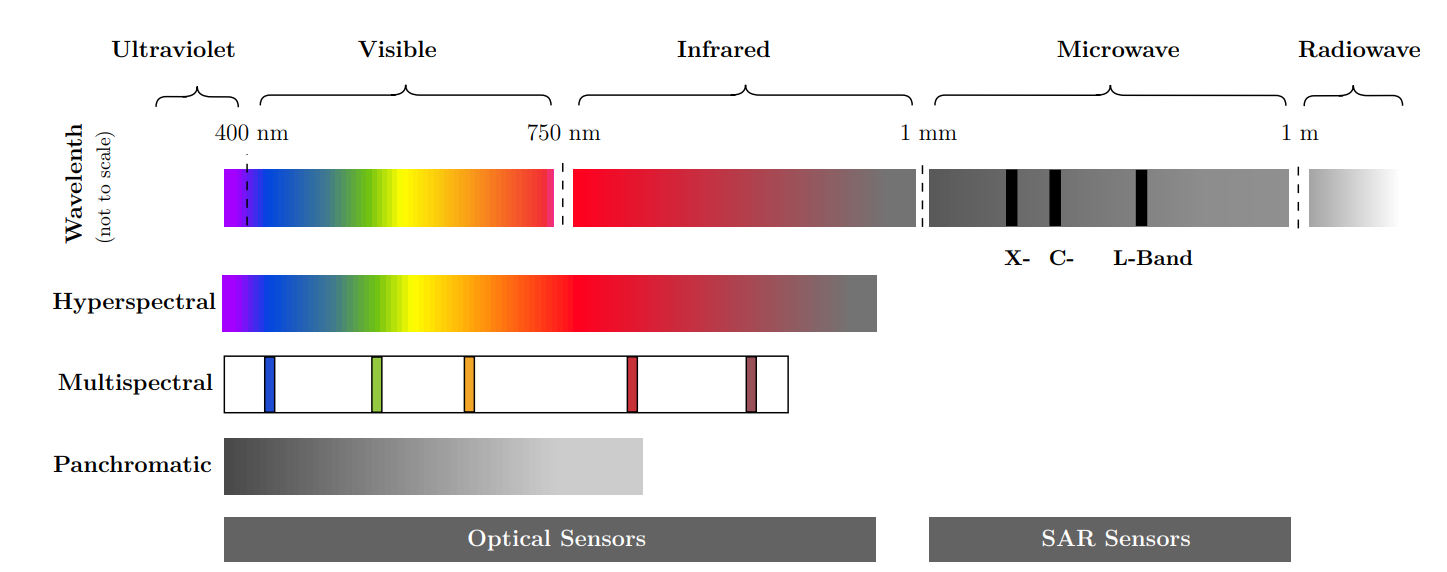
\includegraphics[width=0.9\textwidth]{../../Images/PNG/sensor.png}
    %\decoRule
    \caption[Spectral regions of sensors within the electromagnetic spectrum.]{Spectral regions of optical sensors and radar sensors within the electromagnetic spectrum,~\citep{zhang2022synthetic}.}
    \label{fig:EM-spectrum}
\end{figure}
SAR sensors provide radar images of the Earth’s surface, which are chosen in this work.
Table~\ref{tab:bands} contains the band with the associated frequency and wavelength. 
The wavelength range is very important, since it determines the interaction between radar signals and surfaces, as well as the penetration depth of the microwave
signals.



\setlength{\tabcolsep}{6.0pt}
\begin{table}[!htb]
\caption[Different bands in microwave remote sensing]{\label{tab:bands}Different bands in microwave remote sensing,~\citep{Moreira2013}.}
\centering
\begin{tabular}[t]{cccccc}
\toprule
 \textbf{Band} & \multicolumn{1}{c}{\textbf{Frequency} $\left[\text{GHz}\right]$} & \multicolumn{1}{c}{\textbf{Wavelength} $\left[\text{cm}\right]$} \\
\midrule
Ka & $\,25$--$40$ & $\phantom{-}0.75$--$1.2$ \\
Ku & $\,12$--$17.6$ & $\phantom{-}\,1.7$--$2.5$ \\
X  & $7.5$--$12$  & $2.5$--$4$   \\
C  & $ 3.75$--$7.5$ & $\phantom{-}4$--$8$   \\
S  & $2$--$3.75$   & $\phantom{-}\,8$--$15$    \\
L  & $1$--$2$   & $\phantom{-}15$--$30$   \\
P  & $0.3$--$1$ & $\phantom{-}\,30$--$100$  \\
\bottomrule
\end{tabular}
\end{table}
Table~\ref{tab:spacebornes} gives some examples of commonly used spaceborne SAR sensors, currently in operation. 
These include Radarsat-2 from the Canadian Space Agency (CSA), TerraSAR-X from the German Aerospace Center (DLR), ALOS PALSAR-2 from the Japan Aerospace Exploration Agency (JAXA), and Sentinel-1A/1B from the European Space Agency (ESA) (see Figure~\ref{fig:Sentinel-1}), as well as Gaofen-3 from the China National Space Administration (CNSA).
\begin{figure}[H]
    \centering
    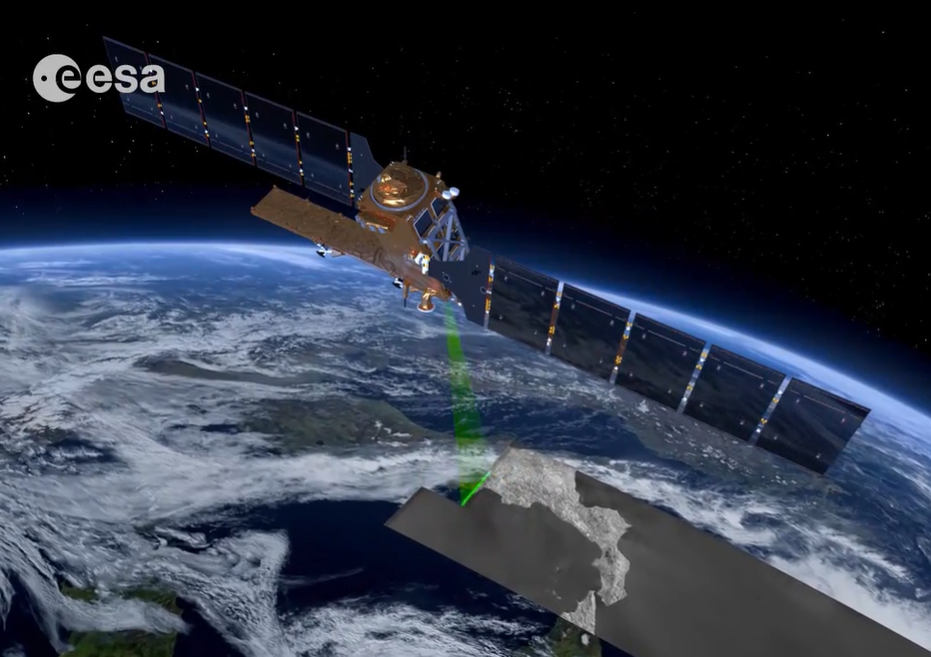
\includegraphics[width=0.6\textwidth]{../../Images/PNG/ESA_radar.png}
    %\decoRule
    \caption[Sentinel-1 radar.]{Sentinel-1 radar, (source \href{https://www.esa.int/Applications/Observing_the_Earth/Copernicus/Sentinel-1/Changing_lands}{ESA}).}
    \label{fig:Sentinel-1}
\end{figure}


\setlength{\tabcolsep}{3.0pt}
\begin{table}[!htb]
\caption[List of operational typical spaceborne SAR systems]{\label{tab:spacebornes}List of operational typical spaceborne SAR systems.}
\centering
\setlength{\extrarowheight}{3.0pt} % 
\begin{tabular}[t]{lclccccc}
\toprule
\textbf{Mission/SAR} & \textbf{Agency} & \textbf{Launch} & \textbf{Band} & \textbf{Resolution} $\left[\text{m}\right]$ & \textbf{Coverage} $\left[\text{km}\right]$ & \textbf{Revisit} $\left[\text{days}\right]$ \\
\midrule
Radarsat-2 & CSA & 2007 & C & 9--100 & 18--500 & 24 \\
TerraSAR-X & DLR & 2007 & X & 0.25--40 & 10--150 & 11 \\
ALOS PALSAR-2 & JAXA & 2014 & L & 1--100 & 25--490 & 14 \\
Sentinel 1A/1B & ESA & 2014/2016 & C & 5--100 & 80--400 & 12 \\
Gaofen-3 & CNSA & 2016 & C & 1--500 & 10--650 & 29 \\
\bottomrule
\end{tabular}
\end{table}

\subsection{Scattering Mechanisms}
A SAR sensor measures the electromagnetic energy that is backscattered from the targets. 
There are lots of factors that can affect the radar backscatter, and they can be divided into two categories.

The first category relates to the SAR parameters, such as the frequency, polarization, and incident angle. If the frequency and
polarization parameters are fixed, the increasing incident angle causes the decreasing backscatter intensity from a homogeneous surface. 
Therefore, the intensity decreases gradually on SAR images from near range to far range. This effect must be taken into consideration during SAR image
interpretation.

The second category relates to the surface parameters, such as the surface roughness, the surface geometry, and the dielectric constant of the
surface. There are three basic groups of scattering mechanisms that can contribute to the returned signal: surface scattering, volume scattering, and hard target scattering.

\subsection{Electromagnetic Polarization}
An electromagnetic wave consists of a magnetic and an electric field.
These two fields are perpendicular to each other and also to the direction of wave propagation.

Apart from frequency, amplitude, and phase, an electromagnetic wave also contains polarization information.
Polarization is defined as the orientation of the oscillating electric field, which can be described in terms of two orthogonal basis vectors.
Electromagnetic waves are generally elliptically polarized, with linear or circular polarization as special cases.

Most of the SAR sensors use linear polarization on both the transmitter and the receiver. 
There are four linear polarization configurations in total:
\begin{itemize}
	\item HH (co-polarization): horizontal transmission and horizontal reception.
	\item HV (cross-polarization): horizontal transmission and vertical reception.
	\item VH (cross-polarization): vertical transmission and horizontal reception.
	\item VV (co-polarization): vertical transmission and vertical reception.
\end{itemize}
Historical SAR satellites carried single-polarized sensors, which support only one linear polarization. More recent sensors provide either dual-polarization
or quad-polarization capabilities. 
For quad-polarization SAR systems, they can transmit H- and V-polarized waveforms and receive both H and V simultaneously.

%An example of polarization is shown in Figure~\ref{}, where three intensity-format C-Band images of a region in Flevoland are observed, with VV and HV polarizations composited into an RGB image.
%An example of polarizations is shown in Figure~\ref{fig:pol}, from Sentinel-1 radar images in C-Band and intensity format of a region in Flevoland.
 Figure~\ref{fig:pol} \ref{fig:1a}--\ref{fig:2a} shows VH and VV polarization from Sentinel-1 radar images in C-Band of a region of Flevoland.
\begin{figure}[H]
  \centering
  \begin{subfigure}[b]{0.45\textwidth}
    \centering
    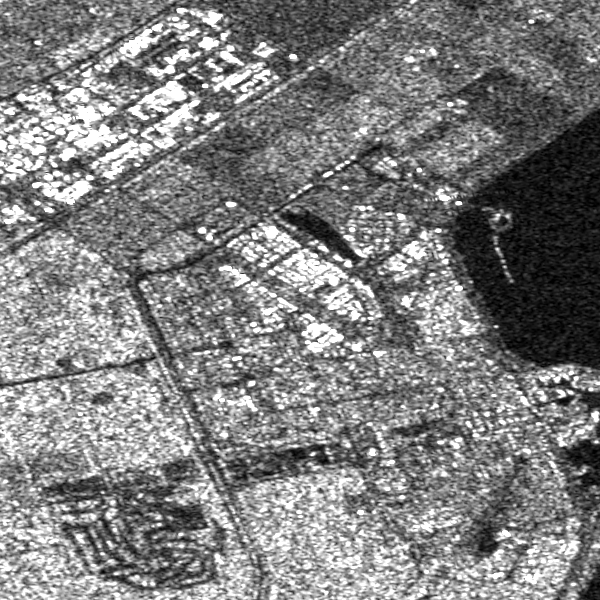
\includegraphics[width=.8\textwidth]{../../Images/PNG/Amplitude_VH.png}
    \caption{Cross-polarization (VH)}
    \label{fig:1a}
  \end{subfigure}
  \hfill
  \begin{subfigure}[b]{0.45\textwidth}
    \centering
    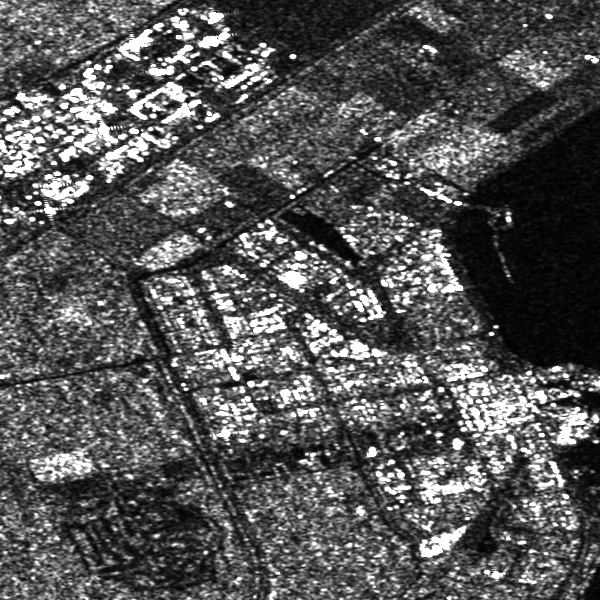
\includegraphics[width=.8\textwidth]{../../Images/PNG/Intensity_VV.png}
    \caption{Co-polarization (VV) }
    \label{fig:2a}
  \end{subfigure}
  %\hfill
  %\begin{subfigure}[b]{0.3\textwidth}
    %\centering
    %\includegraphics[width=\textwidth]{example-image-c}
    %\caption{}
    %\label{fig: Third figure}
  %\end{subfigure}
  \caption{Polarization in radar systems}
  \label{fig:pol}
\end{figure}




\section{SAR Image Acquisition}
SAR sensors utilize a single antenna to emit EM-signals and measure the corresponding magnitude, range and Doppler-shift of these signals in the
backscatter. 
As only a single detector element exists, SAR is based around the concept of synthesizing an aperture in the azimuth direction in order to form a 2-dimensional
image~\citep{Orth2018}. The angle between the SAR antenna and an object on the ground is known as the incidence angle, $\theta$, and it plays a large role in the geometric distortions which are
present in SAR imagery. Due to this imaging concept, the SAR image is formed along the slant range, where each pixel represents the accumulation of backscatter from points which are the same distance away from the sensor~\citep{cumming2005digital}. The acquisition geometry of  SAR sensors is depicted in Figure~\ref{fig:Sentinel-1}.

\begin{figure}[H]
    \centering
    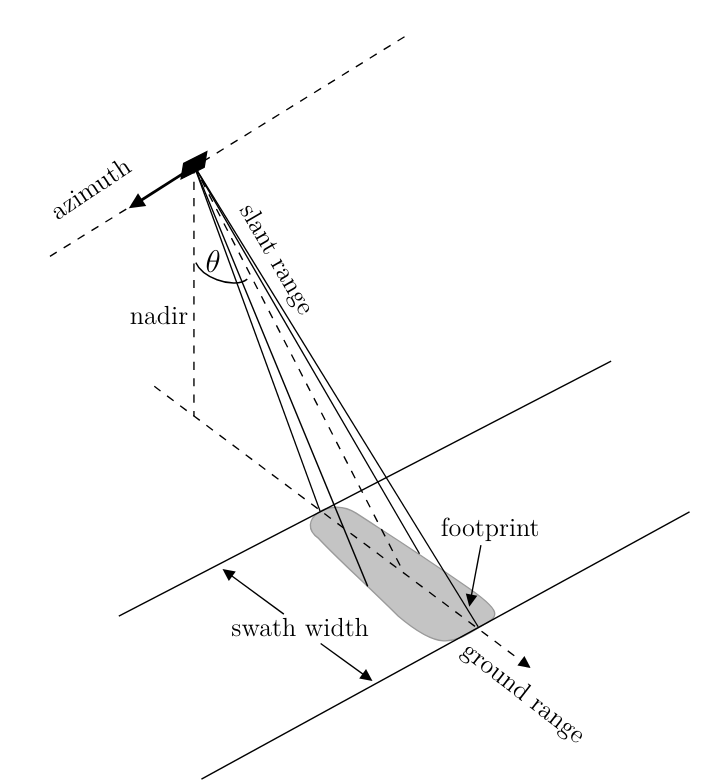
\includegraphics[width=0.5\textwidth]{../../Images/PNG/image_adquisition.png}
    %\decoRule
    \caption[Sentinel-1 radar.]{SAR image acquisition geometry,~\citep{hughes2020deep}.}
    \label{fig:Sentinel-1}
\end{figure}

\subsection{SAR resolution}
The resolution of the SAR image is one of the most important characteristics of the SAR system. 
SAR data pixels are characterized by spatial and temporal resolutions. Spatial resolution is defined as the ability of the SAR system to distinguish between two closely targets.
In SAR systems, there are two resolutions, azimuth resolution, and range resolution. 
Another resolution that should be taken into account when applying a multi-temporal time series analysis of the SAR data is the temporal resolution. 
It is determined by the revisit time of the SAR sensor at the same imaged area.


\subsection{Speckle Noise}
 
The interference of waves reflected during the acquisition process of SAR  images give rise to a multiplicative and non-Gaussian noise that characterizes them
and is known as speckle noise~\citep{oliver2004understanding}.
Since many elemental scatterers are located in one resolution cell, the final scattering response from the resolution cell is the coherent sum of thousands of individual scattering events.
The mutual interference results in a certain fluctuation in the amplitude and phase of the synthesized EM wave vectors, which make the “salt-and-pepper” noise  appear. 
%In the actual SAR images, speckle noise exists in the form of a multiplicative noise, which is manifested in the image as a drastic change in the image intensity.

%The interpretation of the SAR image is challenging due to the geometrical properties of the SAR imaging system and
%to the presence of speckle. Indeed, speckle is a multiplicative noise produced by interference among the backscatterings of
%the objects inside a resolution cell of the sensor~\citep{Argenti2013}.

The statistical distribution of the speckle is well known under certain conditions. Three main cases can be considered:
homogeneous, heterogeneous, and extremely heterogeneous areas. Homogeneous areas (such as fields, pasture, water bodies, etc)
are characterized by the lack of dominant scatterers, and the surface  can be considered stationary. This is the case of the
\textit{fully developed hypothesis for the speckle}~\citep{Frery1997}.

In Figure~\ref{fig:speckle}, SAR images depict speckle, a characteristic of SAR data due to its coherent imaging process. 
The images distinguishes between fully developed speckle in homogeneous regions (Figure~\ref{fig:speckle} \ref{fig:s1}) and heterogeneous clutter in regions such as urban areas (Figure~\ref{fig:speckle} \ref{fig:s2}).
\begin{figure}[H]
  \centering
  \begin{subfigure}[b]{0.48\textwidth}
    \centering
    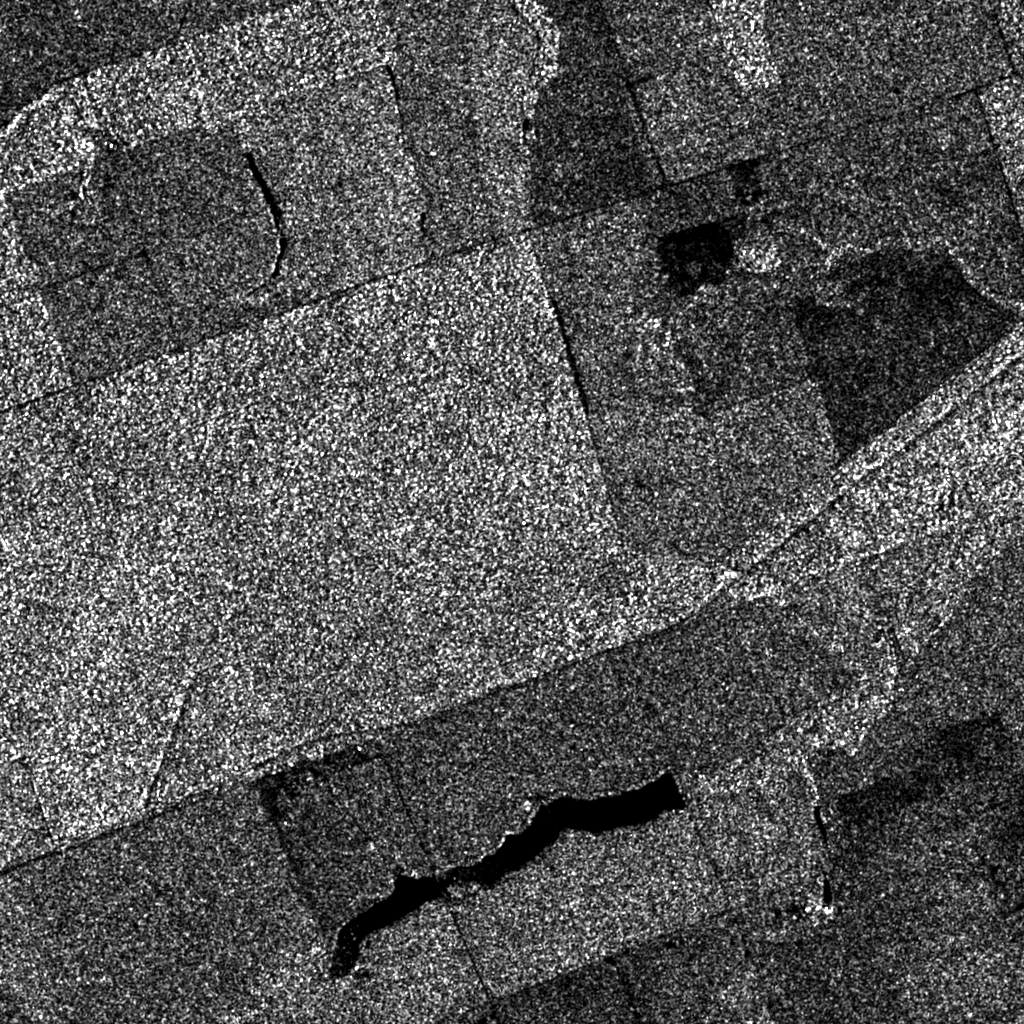
\includegraphics[width=.8\textwidth]{../../Images/PNG/Intensity_MG.png}
    \caption{Fully developed speckle (Homogeneous areas)}
    \label{fig:s1}
  \end{subfigure}
  \hfill
  \begin{subfigure}[b]{0.45\textwidth}
    \centering
    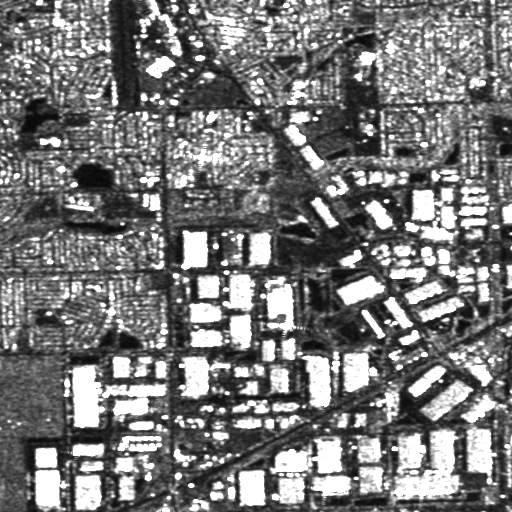
\includegraphics[width=.85\textwidth]{../../Images/PNG/urban_intensity.png}
    \caption{Heterogeneous clutter }
    \label{fig:s2}
  \end{subfigure}
  %\hfill
  %\begin{subfigure}[b]{0.3\textwidth}
    %\centering
    %\includegraphics[width=\textwidth]{example-image-c}
    %\caption{}
    %\label{fig: Third figure}
  %\end{subfigure}
  \caption{SAR image with speckle noise}
  \label{fig:speckle}
\end{figure}

\section{Dataset}
\subsection{Sentinel-1 SAR data processing}
The Sentinel-1 images were obtained from the Alaska Satellite Facility's (ASF) at \url{https://search.asf.alaska.edu/#/} and by the European Space Agency via Copernicus Data Space Ecosystem at \url{https://dataspace.copernicus.eu/}.

The downloaded SAR images were pre-processed using the Sentinel Application Platform (SNAP) Toolbox developed by ESA. 

%The following images describe the preprocessing steps applied to the SAR data: 
The following steps were applied to the SAR data during pre-processing:

\begin{enumerate}
    \item Importing the SAR image into SNAP.
    \item Creating a subset to focus on the area of interest.
    \item Performing Geometric Correction, which includes Range Doppler Terrain Correction.
    \item Exporting the processed data in ENVI format for further analysis.
\end{enumerate}



\begin{figure}[H]
    \centering
    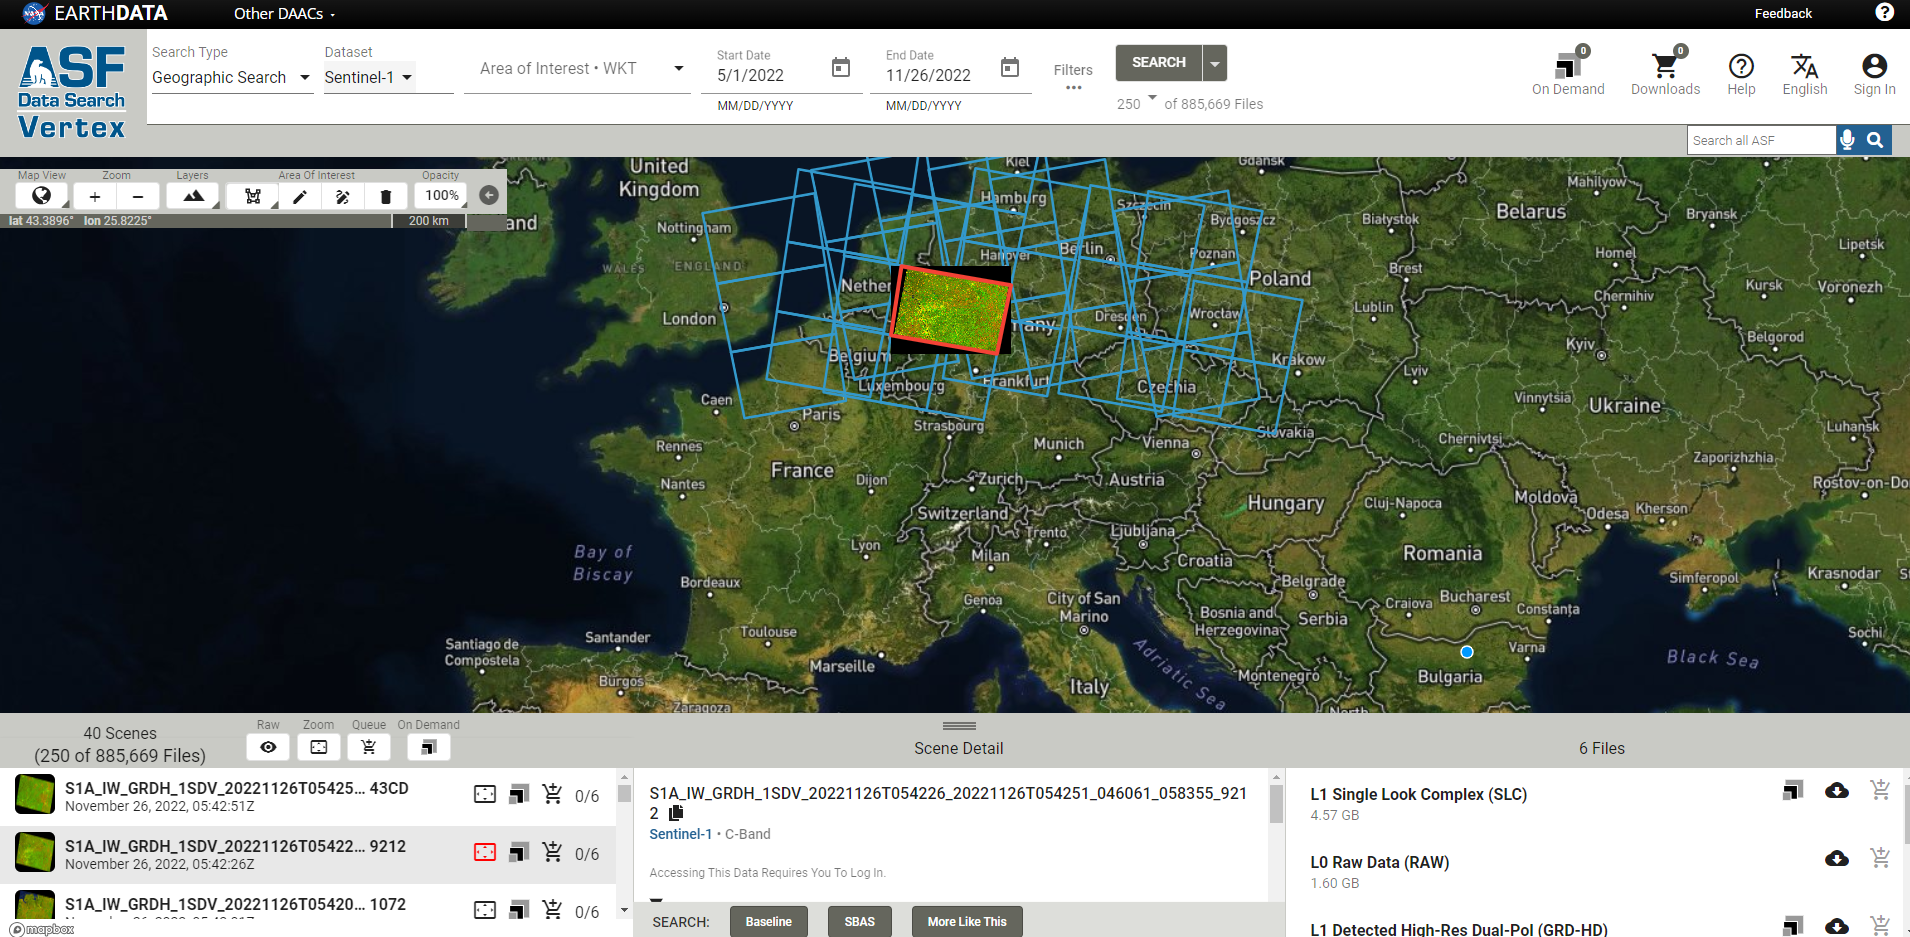
\includegraphics[width=1\textwidth]{../../Images/PNG/alaska1.png}
    %\decoRule
    \caption[Selection of area of interest]{Selection of area of interest.}
    \label{fig:alaska-area}
\end{figure}

\begin{figure}[H]
    \centering
    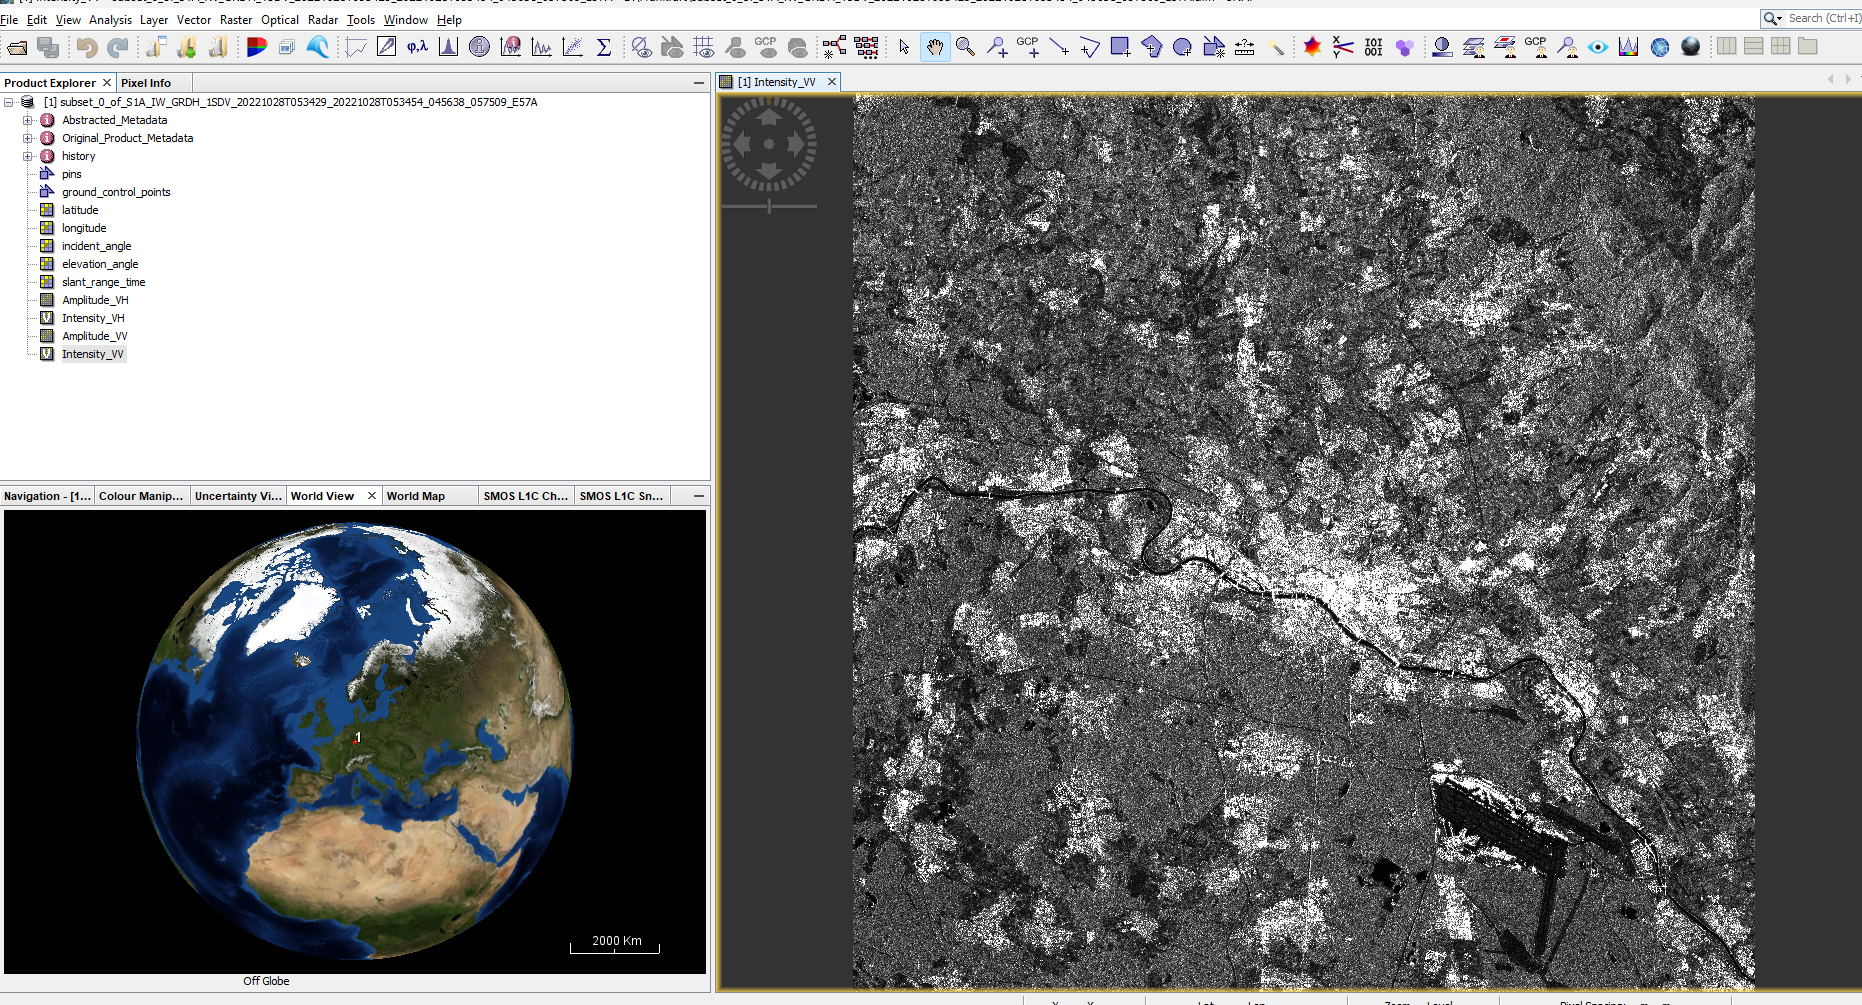
\includegraphics[width=1\textwidth]{../../Images/PNG/snap_1.png}
    %\decoRule
    \caption[SAR Images pre-processing  in the SNAP]{SAR Images pre-processing  in the SNAP.}
    \label{fig:alaska-area2}
\end{figure}


%\subsection*{Example math equations}
%-----------------------------------------------------------
%\begin{align*}
%L(\alpha,  \lambda|  \bm{x})&=\prod_{i=1}^n{f(x_i|\alpha, \lambda )}\\
                                 %&= \prod_{i=1}^n\left[\frac{\lambda^{\alpha}}{\Gamma(\alpha)}\,x_i^{\alpha-1}\exp\left\{-\lambda x_i\right\}\right]\\
%&=\left(\frac{\lambda^{\alpha}}{\Gamma(\alpha)}\right)^n\prod_{i=1}^nx_i^{\alpha-1}\times \exp\left\{-\left(\lambda\sum_{i=1}^n x_i \right)\right\}
%\end{align*}
%%----------------------------------------------------------
%In Figure \ref{fig:undercatch}, in Eq, \eqref{eq:em}.
%\begin{align}
%\label{eq:em}
%\ell(\alpha, \lambda| \bm{x}) &=\log\left[\left(\frac{\lambda^{\alpha}}{\Gamma(\alpha)}\right)^n\prod_{i=1}^nx_i^{\alpha-1}\times \exp\left\{-\left(\lambda\sum_{i=1}^n x_i \right)\right\}\right]\nonumber\\
%&=\log\left(\frac{\lambda^{\alpha}}{\Gamma(\alpha)}\right)^n+\log\left[\prod_{i=1}^nx_i^{\alpha-1}\right]-\lambda\sum_{i=1}^nx_i\nonumber\\
%&=n\log\left(\frac{\lambda^{\alpha}}{\Gamma(\alpha)}\right)+(\alpha-1)\log\prod_{i=1}^nx_i-\lambda\sum_{i=1}^nx_i\nonumber\\
%&=n\log(\lambda^{\alpha})-n\log(\Gamma(\alpha))+(\alpha-1)\sum_{i=1}^n\log(x_i)-\lambda\sum_{i=1}^nx_i\nonumber\\
%&=n\alpha\log \lambda -n\log(\Gamma(\alpha)) +(\alpha-1)\sum_{i=1}^n\log(x_i)-\lambda\sum_{i=1}^nx_i.
	%\end{align}
%----------------------------------------------------------


%-------------------------------------------------------

%\begin{table}[h]
%\centering
%\caption{\label{tab1}Comparação de tempos. }
%\begin{tabular}{l c c }
%\toprule[1pt] \textbf{Amostra (N)} \ \ \  \ \ \  & \textbf{Tempo de Execução (C)}\ \ \ \ \ \ \  &\textbf{Tempo de Execução (Ox)} \\\midrule[0.5pt]
%$20$ & 7.6810 s  &  5.01 s \\
%$30$ & 9.6260 s     & 5.34 s \\
%$50$ &  10.0310 s & 5.99 s \\
%$100$ & 15.5420 s & 8.07 s \\
%$200$ & 20.5860 s & 9.64 s \\
%$500$ & 29.0890  s & 15.12 s \\
%\bottomrule[1pt]
%\end{tabular}
%\caption[Precipitation datasets]{List of datasets used in the analysis of daily precipitation uncertainty carried over i}\label{tab:1}
%\end{table}
%------------------------------------------------------


%\begin{table}[]
%\centering
%\begin{tabular}{@{}llll@{}}
%\toprule
%Dataset name & Period & Spatial res. & Data source \\ \midrule
%E-OBS        & 2000--2016 & \ang{0.25}                            & Station data \\
%EURO4M-APGD  & 2000--2008 & \SI{5}{\kilo\metre}                   & Station data \\
%HMR          & 2000--2013 & \SI{5.5}{\kilo\metre}                 & Reanalysis \\
%ARCIS        & 2000--2015 & \textasciitilde{} \SI{5}{\kilo\metre} & Station data \\
%CHIRPS       & 2000--2016 & \ang{0.05}                            & Station data + satellite \\
%CPC          & 2000--2016 & \ang{0.5}                             & Station data \\
%CMORPH       & 2000--2016 & \ang{0.25}                            & Satellite \\
%PERSIANN-CDR & 2000--2016 & \ang{0.25}                            & Satellite \\ \bottomrule
%\end{tabular}
%\caption[ Italy]{List of datasets used in the analysis of daily precipitation uncertainty  references.}\label{tab:2}
%\end{table}




 
%\chapter{Data}\label{chp:itaobs}

\chapter{Methodology} \label{chp:methods}

\section{Statistical Modeling of Intensity SAR
data}\label{statistical-modeling-of-intensity-sar-data}

The primary models for intensity SAR data include the Gamma and
\(\mathcal{G}_I^0\) distributions~\citep{Frery1997}. The first is
suitable for fully developed speckle and is a limiting case of the
second model. This is interesting due to its versatility in accurately
representing regions with different roughness
properties~\citep{Cassetti2022}. We denote
\(Z \sim \Gamma_{\text{SAR}}(L, \mu)\) and
\(Z \sim \mathcal{G}_I^0(\alpha, \gamma, L)\) to indicate that \(Z\)
follows the distributions characterized by the respective probability
density functions (pdfs): \begin{align}
    f_Z(z;L, \mu\mid \Gamma_{\text{SAR}})&=\frac{L^L}{\Gamma(L)\mu^L}z^{L-1}\exp\left\{-Lz/\mu\right\} \mathbbm 1_{\mathbbm R_+}(z)\label{E:gamma1}\\
    \intertext{ and }
    f_Z(z; \alpha, \gamma, L \mid \mathcal{G}_I^0)&=\frac{L^L\Gamma(L-\alpha)}{\gamma^{\alpha}\Gamma(-\alpha)\Gamma(L)}\cdot\frac{z^{L-1}}{(\gamma+Lz)^{L-\alpha}} \mathbbm 1_{\mathbbm R_+}(z),\label{E:gi01}
\end{align} where \(\mu > 0\) is the mean, \(\gamma > 0\) is the scale,
\(\alpha < 0\) measures the roughness, \(L \geq 1\) is the number of
looks, \(\Gamma(\cdot)\) is the gamma function, and
\(\mathbbm 1_{A}(z)\) is the indicator function of the set \(A\).

The \(r\)th order moments of the \(\mathcal{G}_I^0\) model are
\begin{equation}
E\big(Z^r\mid \mathcal{G}_I^0\big)  = \left(\frac{\gamma}{L}\right)^r\frac{\Gamma(-\alpha-r)}{\Gamma(-\alpha)}\cdot\frac{\Gamma(L+r)}{\Gamma(L)}, 
    \label{E:rmom}
\end{equation} provided \(\alpha <-r\), and infinite otherwise.
Therefore, assuming \(\alpha<-1\), its expected value is
\begin{equation}
    \mu=\left(\frac{\gamma}{L}\right)\frac{\Gamma(-\alpha-1)}{\Gamma(-\alpha)}\cdot\frac{\Gamma(L+1)}{\gamma(L)}=-\frac{\gamma}{\alpha+1}.
\end{equation}

Although the \(\mathcal{G}_I^0\) distribution is defined by the
parameters \(\alpha\) and \(\gamma\), in the SAR
literature~\citep{Nascimento2010} the texture \(\alpha\) and the mean
\(\mu\) are usually used. 
Reparametrizing~\eqref{E:gi01} with \(\mu\),
and denoting this model as \(G_I^0\) we obtain: 
\begin{equation}
        f_Z\big(z; \mu, \alpha, L\mid G_I^0\big) = \frac{L^L\Gamma(L-\alpha)}{\big[-\mu(\alpha+1)\big]^{\alpha}\Gamma(-\alpha)\Gamma(L)} \frac{z^{L-1}}{\big[-\mu(\alpha+1)+Lz\big]^{L-\alpha}}.\label{E:gi02}
\end{equation}


\section{The Shannon Entropy}\label{the-shannon-entropy}

The parametric representation of Shannon entropy for a system described
by a continuous random variable is: \begin{equation}
  \label{E:entropy2}
  H(Z)=-\int_{-\infty }^\infty \ f(z)\ln f(z)\, \mathrm{d}z,
\end{equation} here, \(f(\cdot)\) is the pdf that characterizes the
distribution of the real-valued random variable \(Z\).

Using~\eqref{E:entropy2}, we obtain the Shannon entropy of \(\Gamma_{\text{SAR}}\) in~\eqref{E:gamma1} and \(G_I^0\) in~\eqref{E:gi02}:
\begin{equation}
\label{E:E-gamma}
H_{\Gamma_{\text{SAR}}}(L, \mu) =   L -\ln L+\ln\Gamma(L)+(1-L)\psi^{(0)}(L) + \ln \mu, 
\end{equation}
 %\begin{multline}
%\label{E:E-GIO}
%H_{\mathcal{G}_I^0}(\mu, \alpha, L) =\underbrace{L -\ln L+\ln\Gamma(L)+(1-L)\psi^{(0)}(L) +\ln \mu}_{H_{\Gamma_{\text{SAR}}}} \\
%- \underbrace{\ln\Gamma(L-\alpha)+ (L-\alpha) \psi^{(0)}(L-\alpha)-(1-\alpha)\psi^{(0)}(-\alpha)+\ln (-1-\alpha)+\ln\Gamma(-\alpha)-L}_{\phi(\alpha)},
%\end{multline} 
\begin{multline}
\label{E:E-GIO}
H_{G_I^0}(\mu, \alpha, L) =\underbrace{L -\ln L+\ln\Gamma(L)+(1-L)\psi^{(0)}(L) +\ln \mu}_{H_{\Gamma_{\text{SAR}}}} -\ln\Gamma(L-\alpha)\\
+ (L-\alpha) \psi^{(0)}(L-\alpha)-(1-\alpha)\psi^{(0)}(-\alpha)+\ln (-1-\alpha)+\ln\Gamma(-\alpha)-L,
\end{multline}
where \(\psi^{(0)}(\cdot)\) is the digamma function. 
 
Figure~\ref{fig:all_H} \ref{fig:H1} shows the theoretical entropy $H_{\Gamma_{\text{SAR}}}(L, \mu)$ as a function of $\mu$ for different values of $L$, while Figure~\ref{fig:all_H} \ref{fig:H2} shows the theoretical entropy $H_{G_I^0}(\mu, \alpha, L)$ as a function of both $\mu$ and $\alpha$, likewise considering varying $L$. 
\begin{figure}[htb]
  \centering
  \begin{subfigure}[b]{0.35\textwidth}
    \centering
    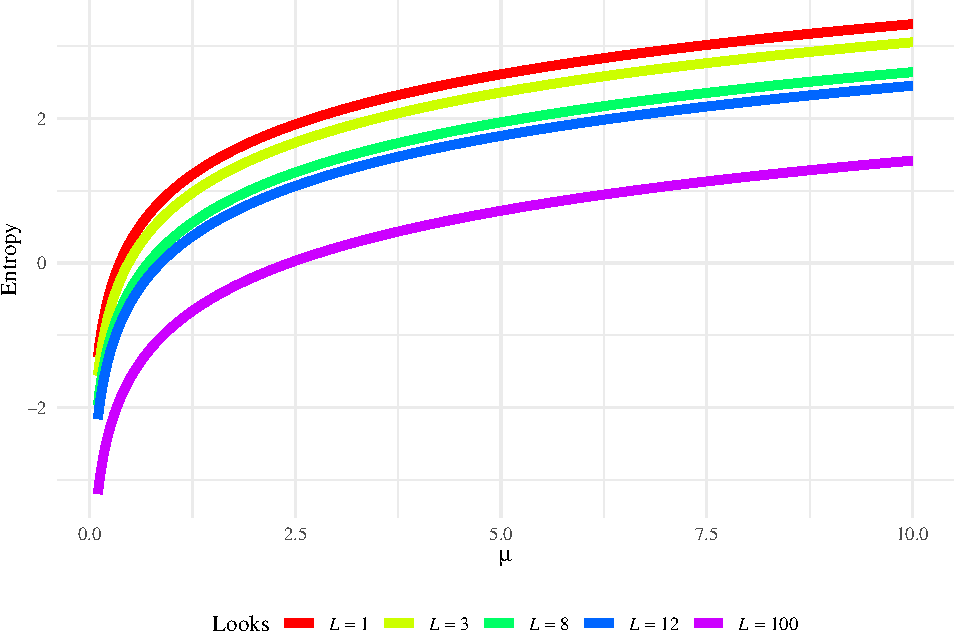
\includegraphics[width=1.5\textwidth]{../../Figures/PDF/PlotGammaSAR-1}
    \caption{The Shannon Entropy of $\Gamma_{\text{SAR}}$.}
    \label{fig:H1}
  \end{subfigure}
  \hfill
  \begin{subfigure}[b]{0.6\textwidth}
    \centering
    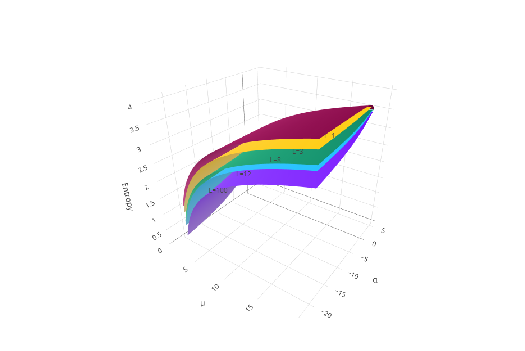
\includegraphics[width=12cm, height=7cm]{../../Figures/PDF/3d_lab}
    \caption{The Shannon Entropy of $G_I^0$.}
    \label{fig:H2}
  \end{subfigure}
  \caption{Theoretical entropies for $\Gamma_{\text{SAR}}$ and $G_I^0$ distributions.}
  \label{fig:all_H}
\end{figure}
We see that the entropy of a random variable following the $\Gamma_{\text{SAR}}$ model depends on the logarithm of the mean $\mu$.  
From the 3D plot, we observe how variations in $\mu$, $\alpha$, and $L$ collectively affect the entropy of the $G_I^0$ distribution, allowing  the identification of regions of high or low entropy.

Additionally, the expression~\eqref{E:E-GIO} can be written as: $H_{G_I^0}(\mu, \alpha, L)=H_{\Gamma_{\text{SAR}}}+\phi(\alpha, L)$. Thus, for $L\geq1$ known, and as \(\alpha\to-\infty\) we have that $H_{G_I^0}\approx H_{\Gamma_{\text{SAR}}}$. 
Figure~\ref{fig:Plot_GI0_to_gamma1}, shows the behavior of the entropy
of \(G_I^0\) as a function of $\mu$ when \(\alpha \in \left\{-\infty, -20, -8, -3\right\}\) and $L=8$,
where the approximation to the entropy of \(\Gamma_{\text{SAR}}\) can be
observed when \(\alpha\) assumes large negative values. In an
interpretative sense, we can conclude that the more heterogeneous (high
values of \(\alpha\)) the SAR region is, the higher the value of entropy
(or degree of disorder). It is worth noting that this conclusion
confirms what is written in the SAR literature.


\begin{figure}[htb]

{\centering 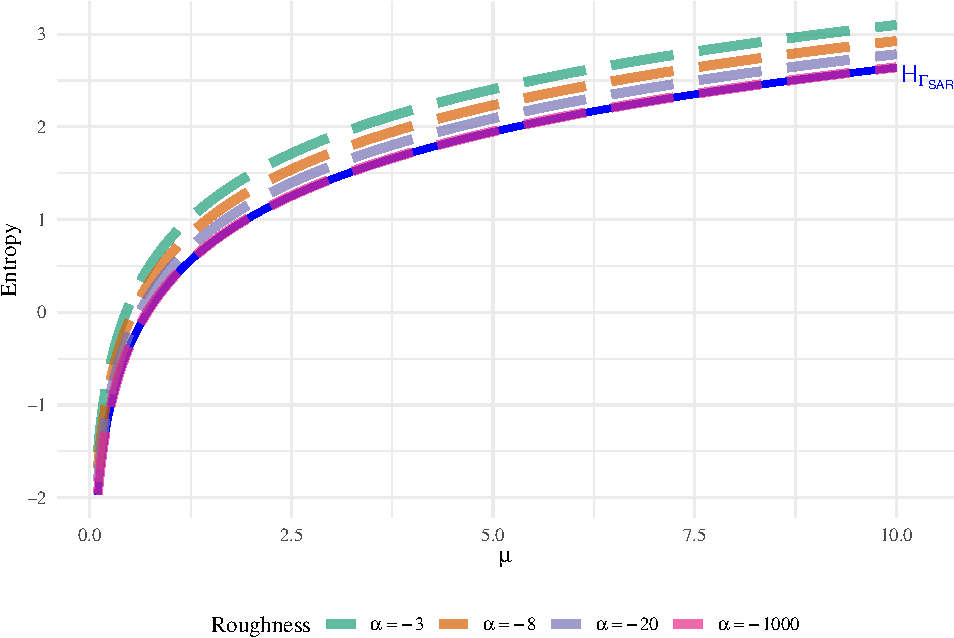
\includegraphics[width=0.7\linewidth]{../../Figures/PDF/Plot_GI0_to_gamma1-1} 

}

\caption{$H_{ G_I^0}$ converges to the $H_{\Gamma_{\text{SAR}}}$ when $\alpha\to-\infty$, with $L=8$.}\label{fig:Plot_GI0_to_gamma1}
\end{figure}

\subsection{Estimation of the Shannon
Entropy}\label{estimation-of-the-shannon-entropy}

The problem of the non-parametric estimation of \(H(Z)\) has been
studied by many authors,
including~\citep{vasicek1976test,correa1995new,Wieczorkowski1999,Yee2015,AlOmari2019}.
Their proposals use estimators based on differences between order
statistics: spacings.

\citet{vasicek1976test} introduced one of the first
non-parametric estimators based on spacings. Under the assumption that
\(\bm{Z}=(Z_1, Z_2,\ldots,Z_n)\) is a random sample from the
distribution \(F(z)\), the estimator is defined as: \begin{equation}
\label{E:Vas}
    \widehat{H}_{\text{V}}(\bm{Z})=\frac{1}{n}\sum_{i=1}^{n}\ln\left[\frac{n}{2m}\left(Z_{(i+m)}-Z_{(i-m)}\right)\right],
    \end{equation} where \(m<n/2\) is a positive integer,
\(Z_{(1)}\leq Z_{(2)}\leq\dots\leq Z_{(n)}\) are the order statistics,
and \(Z_{(i+m)}-Z_{(i-m)}\) is the \(m\)-spacing, in which
\(Z_{(i)}= Z_{(1)}\) if \(i<1\), \(Z_{(i)}= Z_{(n)}\) if \(i>n\).

Several authors have explored adaptations  to Vasicek's estimator. We consider the following entropy estimators variants, as discussed by~\citep{AlOmari2016,Cassetti2022}.

\citet{Bert1992} proposed a new estimator of entropy given by:
 \begin{equation}
\label{E:VanEs}
	\widehat{H}_{\text{VE}}(\bm{Z})=\frac{1}{n-m}\sum_{i=1}^{n-m}\log\left[\frac{n+1}{m}\left(Z_{(i+m)}-Z_{(i)}\right)\right]	+\sum_{k=m}^n\frac{1}{k}+\log\frac{m}{n+1}.
\end{equation}
Under some conditions, Van Es proved asymptotic normality of this estimator.

\citet{Ebrahimi1994} adjusted the weights of Vasicek's estimator, in order to take into account the fact that the differences are truncated around the smallest and the largest data points.
 Specifically, $Z_{(i+m)}-Z_{(i-m)}$ is substituted with  $Z_{(i+m)}-Z_{(1)}$ when $i \leq m$ and $Z_{(i+m)}-Z_{(i-m)}$ is replaced by $Z_{(n)}-Z_{(i-m)}$ when $i \geq n-m+1$. Their estimator is given by:
  \begin{equation}
	\label{E:Ebrahimi}
  \widehat{H}_{\text{E}}(\bm{Z})=\frac{1}{n} \sum_{i=1}^n \log \left[\frac{n}{c_i m}\left(Z_{(i+m)}-Z_{(i-m)}\right)\right],
  \end{equation} where \[
  c_i=\begin{cases}1+(i-1) / m & \text { if } \quad 1 \leq i \leq m, \\ 2 & \text { if }\quad m+1 \leq i \leq n-m,\\ 1+(n-i) / m & \text { if }\quad n-m+1 \leq i \leq n.\end{cases}
  \]

 \citet{correa1995new} suggested another modification of Vasicek's estimator. 
In estimation the density $f$ of $F$ in the interval $\left(Z_{(i-m)}, Z_{(i+m)}\right)$ he used a local linear model based on $2 m+1$ points: $F\left(Z_{(j)}\right)=a+b Z_{(j)}+\varepsilon, j=m-i, \ldots, m+i$. This yields a following estimator:
  \begin{equation}
	\label{E:Correa}
  \widehat{H}_{\text{C}}(\bm{Z})=-\frac{1}{n} \sum_{i=1}^n \log \frac{\sum_{j=i-m}^{i+m}(j-i)\left(Z_{(j)}-\overline{Z}_{(i)}\right)}{n\sum_{j=i-m}^{i+m}\left(Z_{(j)}-\overline{Z}_{(i)}\right)^2},
  \end{equation} where
  \(\widebar{Z}_{(i)}=(2 m+1)^{-1} \sum_{j=i-m}^{i+m} Z_{(j)}\),
  \(m< \frac{n}{2}\), \(Z_{(i)}=Z_{(1)}\) for \(i<1\) and
  \(Z_{(i)}=Z_{(n)}\) for \(i>n\). Based on simulations, he showed that
  his estimator has a smaller mean square error than Vasicek's approach.
	
	 
\citet{rohtua} modify the coefficients of~\eqref{E:Ebrahimi} as: 
\begin{equation}
\label{E:NA}
\widehat{H}_{\text{NA}}(\bm{Z})=\frac{1}{n} \sum_{i=1}^n \log \left[\frac{n}{a_i m}\left(Z_{(i+m)}-Z_{(i-m)}\right)\right],
\end{equation}
where
$$
a_i=\begin{cases}
1 & \text { if } \quad 1 \leq i \leq m, \\
2 & \text { if } \quad m+1 \leq i \leq n-m, \\
1 & \text { if } \quad n-m+1 \leq i \leq n,
\end{cases}
$$
and $Z_{(i-m)}=Z_{(1)}$ for $i \leq m$ and $Z_{(i+m)}=Z_{(n)}$ for $i \geq n-m$.

\citet{IbrahimAlOmari2014} suggested the following estimator:
	\begin{equation}
\label{E:AO}
  \widehat{H}_{\text{AO}}(\bm{Z})=\frac{1}{n} \sum_{i=1}^n \log \left[\frac{n}{\omega_i m}\left(Z_{(i+m)}-Z_{(i-m)}\right)\right],
 \end{equation}
	where \[
  \omega_i= \begin{cases}3/2 & \text { if }\quad 1 \leq i \leq m, \\ 2 & \text { if }\quad m+1 \leq i \leq n-m, \\ 3/2 & \text { if } \quad n-m+1 \leq i \leq n,\end{cases}
  \] in which \(Z_{(i-m)}=Z_{(1)}\) for \(i \leq m\), and
  \(Z_{(i+m)}=Z_{(n)}\) for \(i \geq n-m\).


These estimators are asymptotically consistent, i.e., they converge in
probability to the true value when \(m,n\rightarrow\infty\) and
\(m/n\rightarrow0\). 



Our experimental setup involves an analysis of bias and mean squared error (MSE) for each estimator with a Monte Carlo
study, using \(1000\) samples from the \(\Gamma_{\text{SAR}}\) distribution of size
\(n\in\left\{9, 25, 49, 81, 121\right\}\), with
\(\mu\in\left\{1, 10, 50, 100\right\}\) and \(L=5\). 
The results are consistent with other situations. We use the
heuristic spacing \(m=\left[\sqrt{n}+0.5\right]\), as recommended in the
literature.
Figure~\ref{fig:Plot_bias_mse_gi0_new_L5}  presents the bias and MSE for each of the non-parametric entropy estimators.  The results are summarized  in Table~\ref{tab:tableL5}.
%\begin{figure}[H]
%{\centering 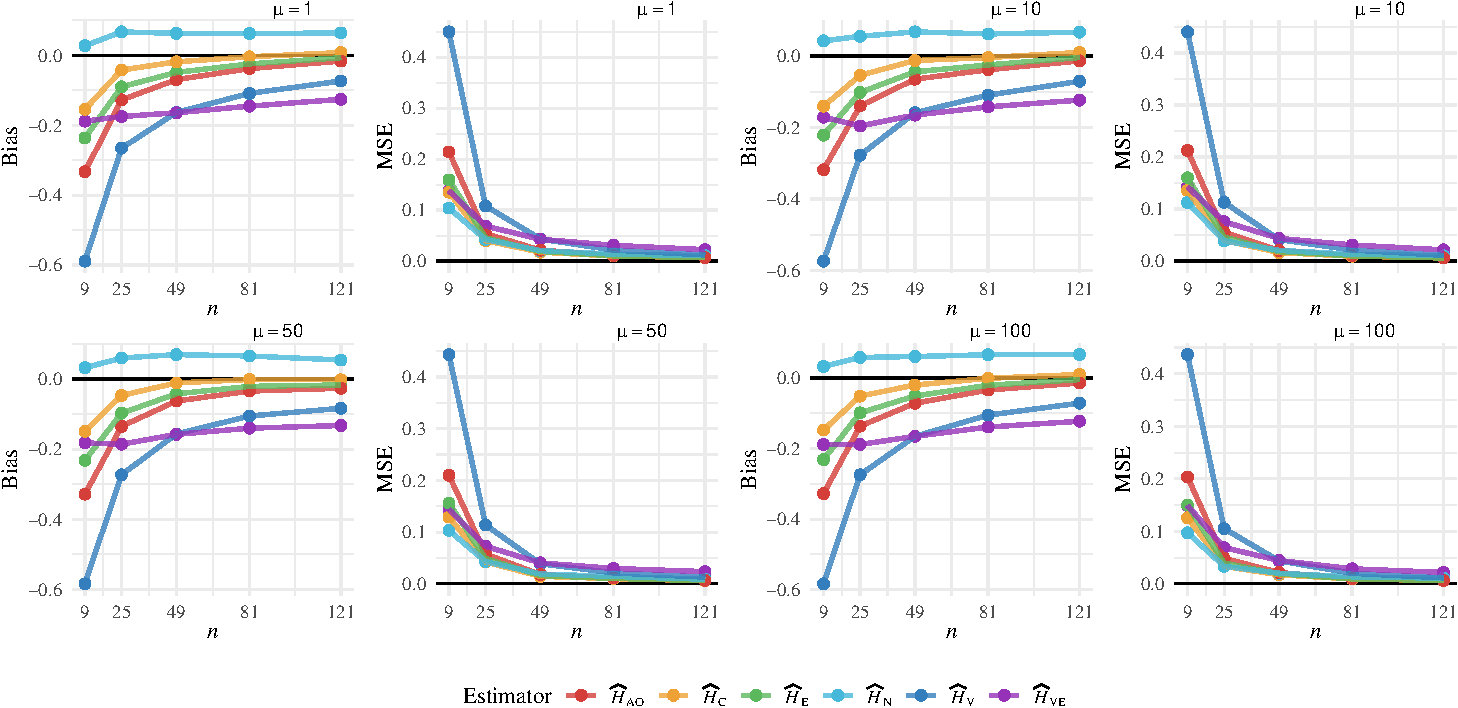
\includegraphics[width=1\linewidth]{../../Figures/PDF/Plot_bias_mse_gi0_new_L2-1} 
%
%}
%\caption{Bias and MSE of the entropy estimators for the $\Gamma_{\text{SAR}}$, with $L=2$.}\label{fig:Plot_bias_mse_gi0_new_L2}
%\end{figure}
\begin{figure}[htb]
{\centering 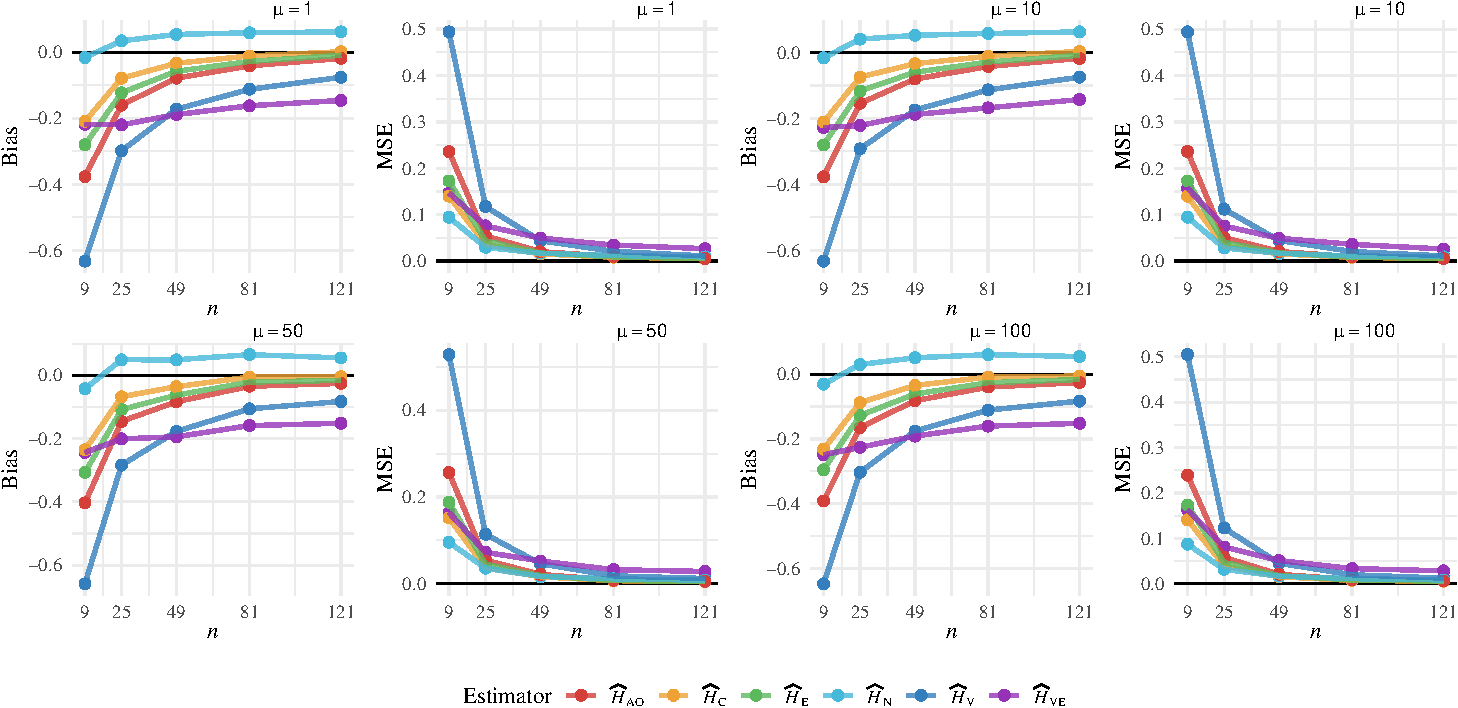
\includegraphics[width=1\linewidth]{../../Figures/PDF/Plot_bias_mse_gi0_new_L5-1} 

}
\caption{Bias and MSE of the entropy estimators for the $\Gamma_{\text{SAR}}$, with $L=5$.}\label{fig:Plot_bias_mse_gi0_new_L5}
\end{figure}



\setlength{\tabcolsep}{6pt}
\begin{table}[htb]
\centering
\caption{\label{tab:tableL5}Bias and MSE of the entropy estimators for the $\Gamma_{\text{SAR}}$, with $L=5$.}
\resizebox{\ifdim\width>\linewidth\linewidth\else\width\fi}{!}{
\begin{tabular}[t]{crllllllllllll}
\toprule
\multicolumn{1}{c}{ } & \multicolumn{1}{c}{ } & \multicolumn{6}{c}{Bias} & \multicolumn{6}{c}{MSE} \\
\cmidrule(l{3pt}r{3pt}){3-8} \cmidrule(l{3pt}r{3pt}){9-14}
\multicolumn{1}{r}{$\bm{\mu}$} & \multicolumn{1}{r}{$\bm{n}$} & \multicolumn{1}{r}{$\bm{\widehat{H}_{\text{V}}}$} & \multicolumn{1}{r}{$\bm{\widehat{H}_{\text{VE}}}$} & \multicolumn{1}{r}{$\bm{\widehat{H}_{\text{E}}}$} & \multicolumn{1}{r}{$\bm{\widehat{H}_{\text{C}}}$} & \multicolumn{1}{r}{$\bm{\widehat{H}_{\text{N}}}$} & \multicolumn{1}{r}{$\bm{\widehat{H}_{\text{AO}}}$} & \multicolumn{1}{r}{$\bm{\widehat{H}_{\text{V}}}$} & \multicolumn{1}{r}{$\bm{\widehat{H}_{\text{VE}}}$} & \multicolumn{1}{r}{$\bm{\widehat{H}_{\text{E}}}$} & \multicolumn{1}{r}{$\bm{\widehat{H}_{\text{C}}}$} & \multicolumn{1}{r}{$\bm{\widehat{H}_{\text{N}}}$} & \multicolumn{1}{r}{$\bm{\widehat{H}_{\text{AO}}}$}\\
\midrule
 & $9$ & $-0.632$ & $-0.218$ & $-0.280$ & $-0.210$ & $-0.016$ & $-0.377$ & $\phantom{-}0.494$ & $\phantom{-}0.147$ & $\phantom{-}0.173$ & $\phantom{-}0.140$ & $\phantom{-}0.094$ & $\phantom{-}0.236$\\

 & $25$ & $-0.298$ & $-0.220$ & $-0.123$ & $-0.079$ & $\phantom{-}0.034$ & $-0.160$ & $\phantom{-}0.117$ & $\phantom{-}0.076$ & $\phantom{-}0.044$ & $\phantom{-}0.036$ & $\phantom{-}0.030$ & $\phantom{-}0.054$\\

 & $49$ & $-0.173$ & $-0.189$ & $-0.058$ & $-0.033$ & $\phantom{-}0.054$ & $-0.079$ & $\phantom{-}0.044$ & $\phantom{-}0.050$ & $\phantom{-}0.017$ & $\phantom{-}0.015$ & $\phantom{-}0.017$ & $\phantom{-}0.020$\\

 & $81$ & $-0.112$ & $-0.162$ & $-0.028$ & $-0.011$ & $\phantom{-}0.059$ & $-0.041$ & $\phantom{-}0.021$ & $\phantom{-}0.035$ & $\phantom{-}0.009$ & $\phantom{-}0.008$ & $\phantom{-}0.012$ & $\phantom{-}0.010$\\

\multirow{-5}{*}[2\dimexpr\aboverulesep+\belowrulesep+\cmidrulewidth]{\centering\arraybackslash 1} & $121$ & $-0.076$ & $-0.146$ & $-0.009$ & $\phantom{-}0.001$ & $\phantom{-}0.061$ & $-0.019$ & $\phantom{-}0.011$ & $\phantom{-}0.027$ & $\phantom{-}0.005$ & $\phantom{-}0.005$ & $\phantom{-}0.009$ & $\phantom{-}0.006$\\
\cmidrule{1-14}
 & $9$ & $-0.633$ & $-0.228$ & $-0.280$ & $-0.211$ & $-0.016$ & $-0.377$ & $\phantom{-}0.494$ & $\phantom{-}0.157$ & $\phantom{-}0.173$ & $\phantom{-}0.140$ & $\phantom{-}0.094$ & $\phantom{-}0.236$\\

 & $25$ & $-0.292$ & $-0.221$ & $-0.117$ & $-0.075$ & $\phantom{-}0.041$ & $-0.154$ & $\phantom{-}0.112$ & $\phantom{-}0.076$ & $\phantom{-}0.040$ & $\phantom{-}0.032$ & $\phantom{-}0.028$ & $\phantom{-}0.050$\\

 & $49$ & $-0.174$ & $-0.188$ & $-0.060$ & $-0.034$ & $\phantom{-}0.052$ & $-0.080$ & $\phantom{-}0.045$ & $\phantom{-}0.049$ & $\phantom{-}0.018$ & $\phantom{-}0.016$ & $\phantom{-}0.017$ & $\phantom{-}0.021$\\

 & $81$ & $-0.113$ & $-0.168$ & $-0.029$ & $-0.011$ & $\phantom{-}0.058$ & $-0.042$ & $\phantom{-}0.021$ & $\phantom{-}0.036$ & $\phantom{-}0.009$ & $\phantom{-}0.008$ & $\phantom{-}0.011$ & $\phantom{-}0.009$\\

\multirow{-5}{*}[2\dimexpr\aboverulesep+\belowrulesep+\cmidrulewidth]{\centering\arraybackslash 10} & $121$ & $-0.075$ & $-0.143$ & $-0.008$ & $\phantom{-}0.003$ & $\phantom{-}0.063$ & $-0.018$ & $\phantom{-}0.011$ & $\phantom{-}0.026$ & $\phantom{-}0.006$ & $\phantom{-}0.005$ & $\phantom{-}0.009$ & $\phantom{-}0.006$\\
\cmidrule{1-14}
 & $9$ & $-0.659$ & $-0.244$ & $-0.307$ & $-0.236$ & $-0.043$ & $-0.403$ & $\phantom{-}0.528$ & $\phantom{-}0.164$ & $\phantom{-}0.188$ & $\phantom{-}0.152$ & $\phantom{-}0.096$ & $\phantom{-}0.256$\\

 & $25$ & $-0.284$ & $-0.201$ & $-0.108$ & $-0.068$ & $\phantom{-}0.049$ & $-0.146$ & $\phantom{-}0.114$ & $\phantom{-}0.073$ & $\phantom{-}0.045$ & $\phantom{-}0.038$ & $\phantom{-}0.036$ & $\phantom{-}0.055$\\

 & $49$ & $-0.178$ & $-0.194$ & $-0.063$ & $-0.036$ & $\phantom{-}0.049$ & $-0.084$ & $\phantom{-}0.046$ & $\phantom{-}0.053$ & $\phantom{-}0.019$ & $\phantom{-}0.016$ & $\phantom{-}0.017$ & $\phantom{-}0.022$\\

 & $81$ & $-0.106$ & $-0.159$ & $-0.022$ & $-0.006$ & $\phantom{-}0.065$ & $-0.035$ & $\phantom{-}0.018$ & $\phantom{-}0.033$ & $\phantom{-}0.008$ & $\phantom{-}0.007$ & $\phantom{-}0.011$ & $\phantom{-}0.008$\\

\multirow{-5}{*}[2\dimexpr\aboverulesep+\belowrulesep+\cmidrulewidth]{\centering\arraybackslash 50} & $121$ & $-0.083$ & $-0.152$ & $-0.016$ & $-0.004$ & $\phantom{-}0.054$ & $-0.026$ & $\phantom{-}0.012$ & $\phantom{-}0.029$ & $\phantom{-}0.006$ & $\phantom{-}0.005$ & $\phantom{-}0.008$ & $\phantom{-}0.006$\\
\cmidrule{1-14}
 & $9$ & $-0.647$ & $-0.249$ & $-0.295$ & $-0.232$ & $-0.031$ & $-0.391$ & $\phantom{-}0.505$ & $\phantom{-}0.163$ & $\phantom{-}0.173$ & $\phantom{-}0.141$ & $\phantom{-}0.087$ & $\phantom{-}0.239$\\

 & $25$ & $-0.303$ & $-0.226$ & $-0.127$ & $-0.088$ & $\phantom{-}0.030$ & $-0.165$ & $\phantom{-}0.123$ & $\phantom{-}0.081$ & $\phantom{-}0.047$ & $\phantom{-}0.039$ & $\phantom{-}0.032$ & $\phantom{-}0.058$\\

 & $49$ & $-0.176$ & $-0.191$ & $-0.061$ & $-0.035$ & $\phantom{-}0.050$ & $-0.082$ & $\phantom{-}0.045$ & $\phantom{-}0.051$ & $\phantom{-}0.018$ & $\phantom{-}0.016$ & $\phantom{-}0.017$ & $\phantom{-}0.021$\\

 & $81$ & $-0.111$ & $-0.160$ & $-0.027$ & $-0.009$ & $\phantom{-}0.060$ & $-0.040$ & $\phantom{-}0.020$ & $\phantom{-}0.034$ & $\phantom{-}0.008$ & $\phantom{-}0.008$ & $\phantom{-}0.011$ & $\phantom{-}0.009$\\

\multirow{-5}{*}[2\dimexpr\aboverulesep+\belowrulesep+\cmidrulewidth]{\centering\arraybackslash 100} & $121$ & $-0.083$ & $-0.152$ & $-0.017$ & $-0.006$ & $\phantom{-}0.054$ & $-0.026$ & $\phantom{-}0.013$ & $\phantom{-}0.029$ & $\phantom{-}0.006$ & $\phantom{-}0.006$ & $\phantom{-}0.009$ & $\phantom{-}0.006$\\
\bottomrule
\end{tabular}}
\end{table}
As shown in the simulation results, the estimators \(\widehat{H}_{\text{C}}\), \(\widehat{H}_{\text{E}}\), and \(\widehat{H}_{\text{AO}}\) show low bias and achieve convergence for samples size larger than 81. These estimators exhibit good behavior in terms of bias and MSE across various parameter combinations.

In contrast, estimator \(\widehat{H}_{\text{N}}\) displays the lowest MSE across all scenarios. However,  the bias remains unchanged and high for sample sizes larger than 25, indicating that the convergence
is not very fast. Additionally, we observe that both \(\widehat{H}_{\text{V}}\) and \(\widehat{H}_{\text{VE}}\) estimators exhibit larger bias and slower convergence compared to their counterparts.  Notably, the \(\widehat{H}_{\text{V}}\) estimator shows the highest MSE.

%We will use improved bootstrap-improved versions because we need them to perform well with small samples.

\subsection{Enhanced estimators with Bootstrap}\label{enhanced-estimators-with-bootstrap}

We extend our exploration of non-parametric entropy estimators by incorporating  bootstrap methodologies, because we need them to perform well with small samples. 
The integration of bootstrap techniques aims to refine the accuracy of non-parametric entropy estimators.

Bootstrap is essentially a resampling algorithm introduced by \citep{Efron1979}. 
It offers a simulation-based approach for estimating various statistics of interest for a random variable.
It can be used in both parametric and nonparametric settings. 
The main idea  consists of creating new datasets from an existing one by resampling with repetition~\citep{Michelucci2021}.

Let us assume that the non-parametric entropy estimator
\(\widehat{H}=\widehat{\theta}(\bm{Z})\) is inherently biased, where \(\bm{Z}=(Z_1, Z_2,\ldots,Z_n)\) is a random sample from a
distribution \(\mathcal{D}\), i.e,:\begin{equation}
\label{Eq:bias1}
\operatorname{Bias}\big(\widehat{\theta}(\bm{Z})\big) = \mathbb{E}\big[\widehat{\theta}(\bm{Z})\big] - \theta \neq 0.
\end{equation} 

Our objective is to devise a unbiased estimator. To achieve this, we introduce an "ideal estimator" \(\widecheck{\theta}(\bm{Z})\) using the bias information from~\eqref{Eq:bias1}:
\begin{align}
\label{Eq:bias2}
\widecheck{\theta}(\bm{Z}) &= \widehat{\theta}(\bm{Z}) - \bias\left(\widehat{\theta}(\bm{Z})\right),\nonumber\\
&=\widehat{\theta}(\bm{Z})-\left[\mathbb{E}\big[\widehat{\theta}(\bm{Z})\big] - \theta\right],\nonumber\\
&=\widehat{\theta}(\bm{Z})+\theta-\mathbb{E}\big[\widehat{\theta}(\bm{Z})\big].
\end{align}
However, \(\widecheck{\theta}(\bm{Z})\) is not yet an estimator, because it depend on the true parameter, but \(\theta\) can be calculated using a non-parametric approach, and the average of individual estimators can be obtained using the bootstrap technique. This leads to the formulation of a new unbiased estimator, denoted as \(\widetilde{H}\), from ~\eqref{Eq:bias2} we have:
\begin{align}
\label{Eq:bias3}
\widetilde{H}%&= \widehat{\theta}(\bm{Z})+\widehat{\theta}(\bm{Z})- \frac{1}{B}\sum_{b=1}^B \widehat{\theta}_b(\bm{Z}^{(b)}),\nonumber\\
= 2\widehat{\theta}(\bm{Z}) - \frac{1}{B}\sum_{b=1}^B \widehat{\theta}_b(\bm{Z}^{(b)}),
\end{align} where \(B\) the number of bootstrap replications. For each iteration \(b\) (from \(1\) to \(B\)), a sample \(\bm{Z}^{(b)}\) is generated, and the corresponding bootstrap estimator \(\widehat{\theta}_b(\bm{Z}^{(b)})\) is calculated. 
This methodology significantly reduces bias, resulting in more accurate and robust entropy estimations. The original estimators of Vasicek~\eqref{E:Vas}, Van Es~\eqref{E:VanEs}, Ebrahimi~\eqref{E:Ebrahimi}, Correa~\eqref{E:Correa}, Noughabi~\eqref{E:NA}, and Al-Omari~\eqref{E:AO}  are now referred to as the proposed bootstrap-improved versions:
\(\widetilde{H}_{\text{V}}\),
\(\widetilde{H}_{\text{VE}}\), 
\(\widetilde{H}_{\text{E}}\),
\(\widetilde{H}_{\text{C}}\),
\(\widetilde{H}_{\text{NA}}\), and 
\(\widetilde{H}_{\text{AO}}\),
respectively.

In order to assess the effectiveness of the bootstrap technique, we present comparisons of the bias and MSE between each original non-parametric entropy estimator and its respective bootstrap-enhanced version, with \(B=200\) bootstrap samples, as shown in Figures~\ref{fig:all_estimator}~\ref{fig:Firstfigure}--\ref{fig:subfig6}.
\begin{figure}[H]
  \centering
  \begin{subfigure}[t]{0.48\textwidth}
    \centering
    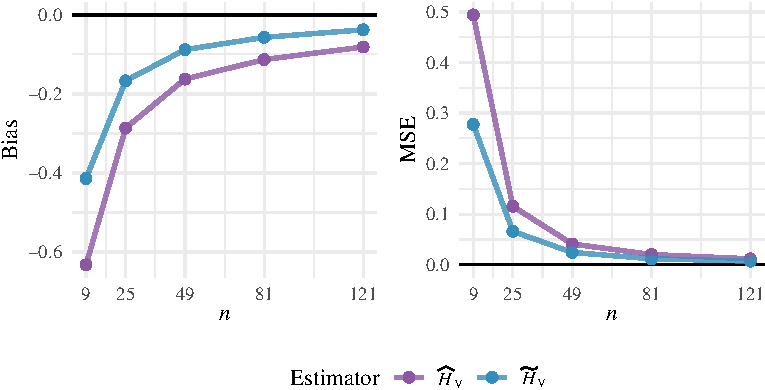
\includegraphics[width=\textwidth]{../../Figures/PDF/Plot_bias_mse_vasicek-1}
    \caption{}
    \label{fig:Firstfigure}
  \end{subfigure}
  \hfill
  \begin{subfigure}[t]{0.48\textwidth}
    \centering
    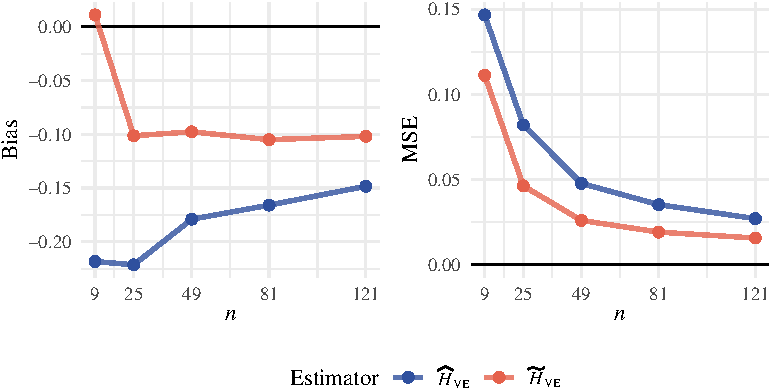
\includegraphics[width=\textwidth]{../../Figures/PDF/Plot_bias_mse_VanEs-1}
    \caption{}
    \label{fig:Secondfigure}
  \end{subfigure}
  %\hfill
  %\begin{subfigure}[b]{0.3\textwidth}
    %\centering
    %\includegraphics[width=\textwidth]{example-image-c}
    %\caption{}
    %\label{fig: Third figure}
  %\end{subfigure}
	
	\begin{subfigure}[t]{0.48\textwidth}
    \centering
    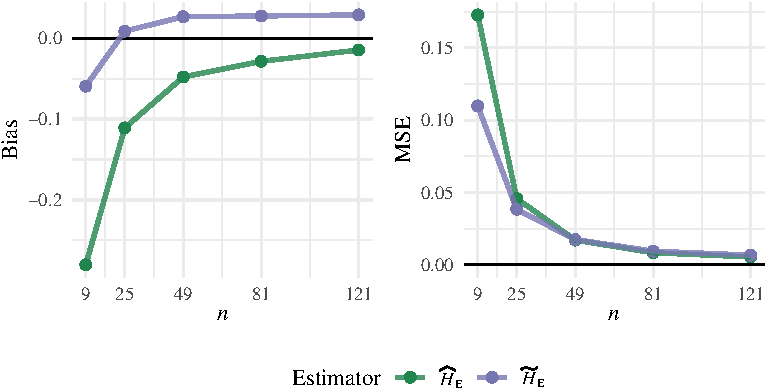
\includegraphics[width=\textwidth]{../../Figures/PDF/Plot_bias_mse_Ebrahimi-1}
    \caption{}
    \label{fig:subfig3}
  \end{subfigure}
  \hfill
  \begin{subfigure}[t]{0.48\textwidth}
    \centering
    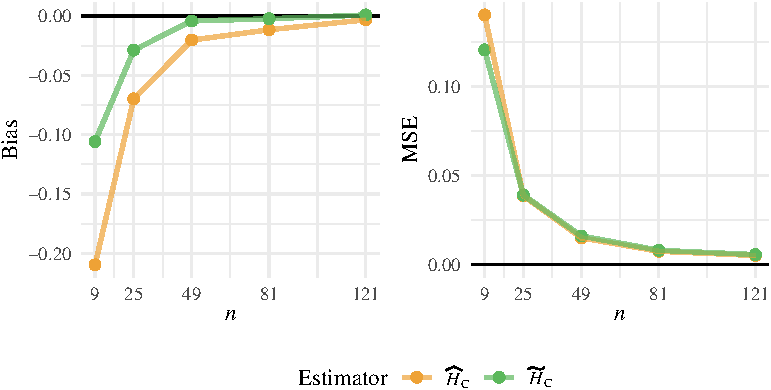
\includegraphics[width=\textwidth]{../../Figures/PDF/Plot_bias_mse_correa-1}
    \caption{}
    \label{fig:subfig4}
  \end{subfigure}
	\begin{subfigure}[t]{0.48\textwidth}
    \centering
    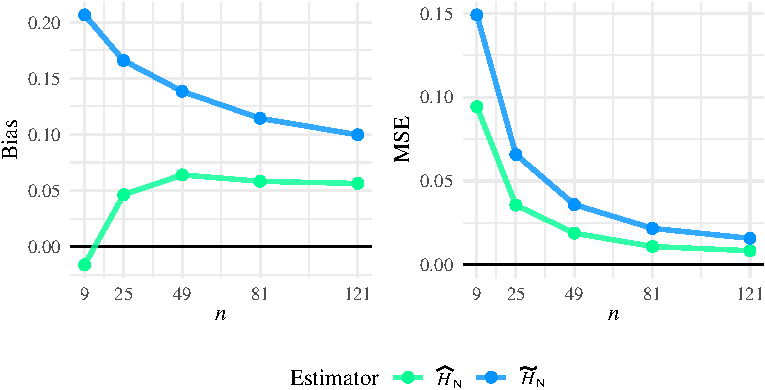
\includegraphics[width=\textwidth]{../../Figures/PDF/Plot_bias_mse_noughabi-1}
    \caption{}
    \label{fig:subfig5}
  \end{subfigure}
  \hfill
  \begin{subfigure}[t]{0.48\textwidth}
    \centering
    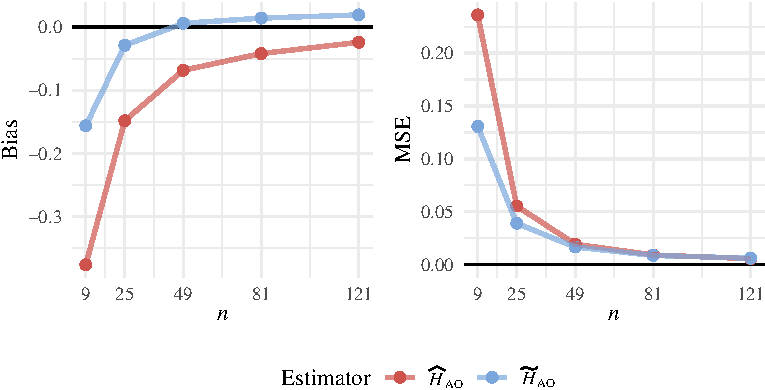
\includegraphics[width=\textwidth]{../../Figures/PDF/Plot_bias_mse_AO-1}
    \caption{}
    \label{fig:subfig6}
  \end{subfigure}
  \caption{Comparing Bias and MSE: original vs. bootstrap estimators, with, $\mu=1$ and $L=5$.}
  \label{fig:all_estimator}
\end{figure}

%I want to write as Fig. \ref{fig:all_estimator} \ref{fig:Firstfigure}--\ref{fig:subfig6}.
Based on previous simulations, the bootstrap technique did not improve the \(\widetilde{H}_{\text{NA}}\) estimator. 
This might occur because the original estimator overestimates the entropy values, showing a positive bias. 
This tendency to overestimate persists with the use of bootstrap, contributing to an increase in bias and MSE.

However, the improvement observed in the most estimators with the application of bootstrap techniques is notable, especially for sample sizes below 81. 
This performance is superior for the \(\widetilde{H}_{\text{C}}\), \(\widetilde{H}_{\text{E}}\), and \(\widetilde{H}_{\text{AO}}\) estimators. 
Therefore, we proceed to perform a comparison of bias and MSE of these three estimators alongside with their original versions, with \(1000\) samples from the \(\Gamma_{\text{SAR}}\) distribution of
size \(n\in\left\{9, 25, 49, 81, 121\right\}\), with \(\mu\in\left\{1, 10\right\}\), \(L=5\), and \(B=200\) bootstrap samples, as shown in Figure~\ref{fig:Plot_bias_mse_gi0} and Table~\ref{tab:table_final}.

%\begin{figure}[htb]
%{\centering 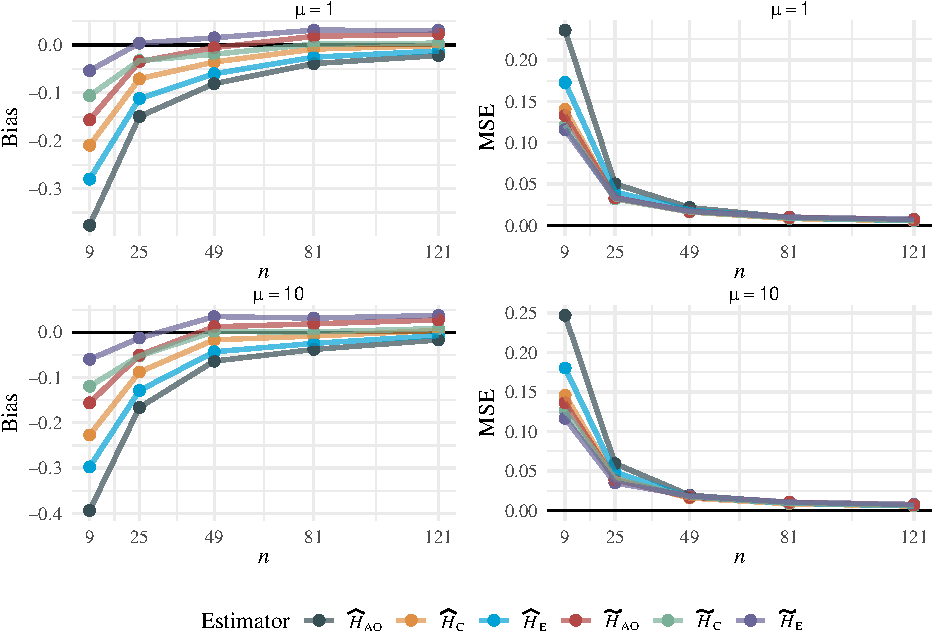
\includegraphics[width=0.7\linewidth]{../../Figures/PDF/Plot_bias_mse_gi0-2}
%}
%\caption{Bias and MSE of the entropy estimators for the $\Gamma_{\text{SAR}}$, with $L=5$.}\label{fig:Plot_bias_mse_gi0}
%\end{figure}
\begin{figure}[htb]
{\centering 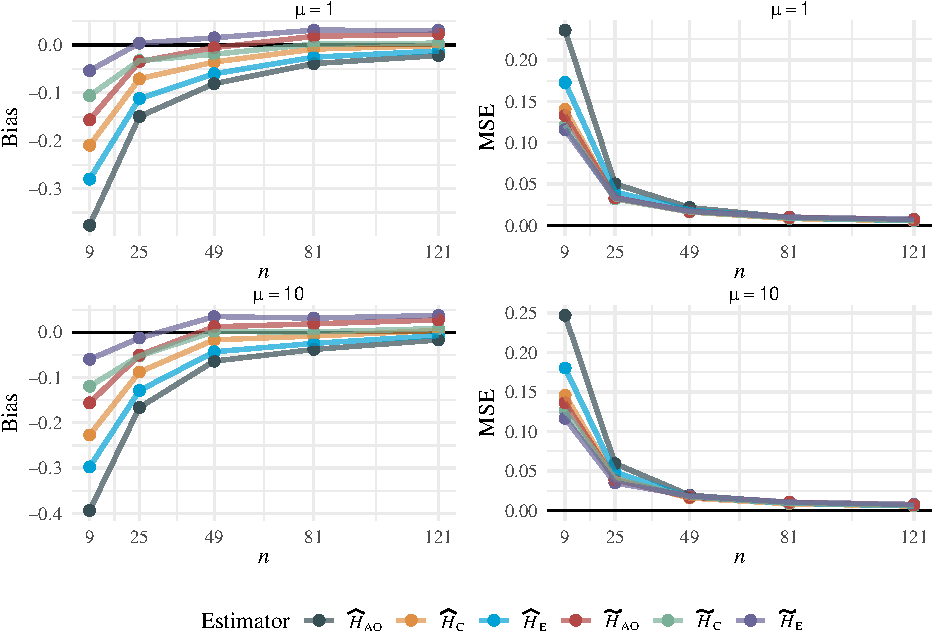
\includegraphics[width=0.8\linewidth]{../../Figures/PDF/Plot_bias_mse_gi0-2} 

}
\caption{Bias and MSE of the entropy estimators for the $\Gamma_{\text{SAR}}$, with $L=5$.}\label{fig:Plot_bias_mse_gi0}
\end{figure}


\setlength{\tabcolsep}{6pt}
\begin{table}[H]
\centering
\caption{\label{tab:table_final}Bias and MSE of the entropy estimators for the $\Gamma_{\text{SAR}}$, with $L=5$.}
\resizebox{\ifdim\width>\linewidth\linewidth\else\width\fi}{!}{
\begin{tabular}[t]{crllllllllllll}
\toprule
\multicolumn{1}{c}{ } & \multicolumn{1}{c}{ } & \multicolumn{6}{c}{Bias} & \multicolumn{6}{c}{MSE} \\
\cmidrule(l{3pt}r{3pt}){3-8} \cmidrule(l{3pt}r{3pt}){9-14}
\multicolumn{1}{r}{$\bm{\mu}$} & \multicolumn{1}{r}{$\bm{n}$} & \multicolumn{1}{r}{$\bm{\widehat{H}_{\text{C}}}$} & \multicolumn{1}{r}{$\bm{\widehat{H}_{\text{E}}}$} & \multicolumn{1}{r}{$\bm{\widehat{H}_{\text{AO}}}$} & \multicolumn{1}{r}{$\bm{\widetilde{H}_{\text{C}}}$} & \multicolumn{1}{r}{$\bm{\widetilde{H}_{\text{E}}}$} & \multicolumn{1}{r}{$\bm{\widetilde{H}_{\text{AO}}}$} & \multicolumn{1}{r}{$\bm{\widehat{H}_{\text{C}}}$} & \multicolumn{1}{r}{$\bm{\widehat{H}_{\text{E}}}$} & \multicolumn{1}{r}{$\bm{\widehat{H}_{\text{AO}}}$} & \multicolumn{1}{r}{$\bm{\widetilde{H}_{\text{C}}}$} & \multicolumn{1}{r}{$\bm{\widetilde{H}_{\text{E}}}$} & \multicolumn{1}{r}{$\bm{\widetilde{H}_{\text{AO}}}$}\\
\midrule
 & $9$ & $-0.210$ & $-0.280$ & $-0.377$ & $-0.106$ & $-0.054$ & $-0.156$ & $\phantom{-}0.140$ & $\phantom{-}0.173$ & $\phantom{-}0.236$ & $\phantom{-}0.121$ & $\phantom{-}0.116$ & $\phantom{-}0.133$\\

 & $25$ & $-0.071$ & $-0.112$ & $-0.149$ & $-0.033$ & $\phantom{-}0.004$ & $-0.035$ & $\phantom{-}0.032$ & $\phantom{-}0.040$ & $\phantom{-}0.050$ & $\phantom{-}0.032$ & $\phantom{-}0.033$ & $\phantom{-}0.033$\\

 & $49$ & $-0.036$ & $-0.060$ & $-0.081$ & $-0.020$ & $\phantom{-}0.015$ & $-0.006$ & $\phantom{-}0.016$ & $\phantom{-}0.019$ & $\phantom{-}0.021$ & $\phantom{-}0.016$ & $\phantom{-}0.017$ & $\phantom{-}0.017$\\

 & $81$ & $-0.009$ & $-0.026$ & $-0.039$ & $\phantom{-}0.002$ & $\phantom{-}0.031$ & $\phantom{-}0.018$ & $\phantom{-}0.008$ & $\phantom{-}0.009$ & $\phantom{-}0.010$ & $\phantom{-}0.009$ & $\phantom{-}0.010$ & $\phantom{-}0.009$\\

\multirow{-5}{*}[2\dimexpr\aboverulesep+\belowrulesep+\cmidrulewidth]{\centering\arraybackslash 1} & $121$ & $-0.001$ & $-0.013$ & $-0.022$ & $\phantom{-}0.004$ & $\phantom{-}0.030$ & $\phantom{-}0.023$ & $\phantom{-}0.005$ & $\phantom{-}0.006$ & $\phantom{-}0.006$ & $\phantom{-}0.006$ & $\phantom{-}0.007$ & $\phantom{-}0.007$\\
\cmidrule{1-14}
 & $9$ & $-0.227$ & $-0.297$ & $-0.394$ & $-0.119$ & $-0.060$ & $-0.156$ & $\phantom{-}0.146$ & $\phantom{-}0.180$ & $\phantom{-}0.247$ & $\phantom{-}0.126$ & $\phantom{-}0.117$ & $\phantom{-}0.136$\\

 & $25$ & $-0.088$ & $-0.129$ & $-0.166$ & $-0.052$ & $-0.013$ & $-0.050$ & $\phantom{-}0.040$ & $\phantom{-}0.048$ & $\phantom{-}0.059$ & $\phantom{-}0.040$ & $\phantom{-}0.035$ & $\phantom{-}0.039$\\

 & $49$ & $-0.017$ & $-0.043$ & $-0.064$ & $\phantom{-}0.001$ & $\phantom{-}0.035$ & $\phantom{-}0.012$ & $\phantom{-}0.016$ & $\phantom{-}0.017$ & $\phantom{-}0.019$ & $\phantom{-}0.018$ & $\phantom{-}0.019$ & $\phantom{-}0.017$\\

 & $81$ & $-0.008$ & $-0.025$ & $-0.038$ & $\phantom{-}0.001$ & $\phantom{-}0.031$ & $\phantom{-}0.019$ & $\phantom{-}0.009$ & $\phantom{-}0.009$ & $\phantom{-}0.010$ & $\phantom{-}0.009$ & $\phantom{-}0.011$ & $\phantom{-}0.010$\\

\multirow{-5}{*}[2\dimexpr\aboverulesep+\belowrulesep+\cmidrulewidth]{\centering\arraybackslash 10} & $121$ & $\phantom{-}0.004$ & $-0.007$ & $-0.017$ & $\phantom{-}0.008$ & $\phantom{-}0.037$ & $\phantom{-}0.027$ & $\phantom{-}0.006$ & $\phantom{-}0.006$ & $\phantom{-}0.006$ & $\phantom{-}0.006$ & $\phantom{-}0.008$ & $\phantom{-}0.007$\\
\bottomrule
\end{tabular}}
\end{table}

\section{Coefficient of variation and a robust
alternative}\label{coefficient-of-variation-and-a-robust-alternative}

The population CV is defined as a ratio of the population standard
deviation \((\sigma)\) to the population mean \((\mu)\): 
\begin{align}
    \text{CV}=\frac{\sigma}{\mu}, \quad \mu \neq 0.
\end{align}

We explore a robust alternative to CV, as described
in~\citep{Ospina2019}, which incorporates the ratio between the mean
absolute deviation from the median (MnAD) and the median, two well-known
robust measures of scale and location, respectively. 
The sample version for the MnAD is defined as \(n^{-1}\sum_{i=1}^n|x_i-\widehat{Q}_2|\),
where \(\widehat{Q}_2\) is an estimate for the median of the population,
which can be approximated by the median of the sample.

\section{Hypothesis Testing}\label{sec:test}

We aim to test the following hypotheses: \[
\begin{cases}
  \mathcal{H}_0: \text{ The data come from the } \Gamma_{\text{SAR}}\text{ law},\\ 
  \mathcal{H}_1:\text{ The data come from the } G_I^0 \text{ distribution}.
\end{cases}
\] We are testing the hypothesis that the data are fully-developed
speckle versus the alternative of data with roughness. As for the
parametric problem, once it is not possible to define the hypothesis
\(\mathcal{H}_0=\alpha=-\infty\), it is impossible to solve this problem
with parametric inference alternatives (such as likelihood ratio, score,
gradient, and Wald hypothesis test). The proposed tests to solve this
physical problem in SAR systems are described below.

\subsection{The Proposed Test Based on Non-parametric
Entropy}\label{the-proposed-test-based-on-non-parametric-entropy}

For a random sample \(\bm{Z}=(Z_1, Z_2,\ldots,Z_n)\) from a distribution
\(\mathcal{D}\), a test statistic is proposed. It is based on an
empirical distribution that arises from the difference between
non-parametrically estimated entropies \(\widetilde{H}(\bm{Z})\) and the
analytical entropy of \(\Gamma_{\text{SAR}}\)~\eqref{E:E-gamma}
evaluated at the logarithm of the sample mean, where \(L\geq 1\) is
known.

Hence, the entropy-based test statistic is defined as: \begin{equation}
\label{Eq:test_e}
S(\bm{Z};L)= \widetilde{H}(\bm{Z})-\left[H_{\Gamma_{\text{SAR}}}(L)+\ln \overline{\bm{Z}}\right].
\end{equation}

This test statistic aims to assess the behavior of the data under the
null hypothesis using the empirical distribution. If the data represent
fully-developed speckle, the density should center around zero, i.e.,
\(S(\bm{Z};L)\approx 0\). Otherwise, the empirical distribution would
shift from zero under the alternative hypothesis, suggesting significant
differences and heterogeneous clutter.

The comparison between the bootstrap-improved estimators is shown in
Table~\ref{tab:table_time}, where the test accuracy under the null
hypothesis is presented alongside running times. The test accuracy is
evaluated through 1000 simulated samples of different sizes, with each
size replicated 100 times using bootstrap resampling.

The processing time is an important feature, especially considering the
application of these estimators to large datasets of SAR images, as seen
in Chapter~\ref{chp:results}.
\setlength{\tabcolsep}{7pt}
\begin{table}[htb]
\centering\centering
\caption{\label{tab:table_time}Test accuracy and processing time for each bootstrap-improved estimator. }
\resizebox{\ifdim\width>\linewidth\linewidth\else\width\fi}{!}{
\small
\begin{tabu} to \linewidth {>{\centering}X>{\centering}X>{\centering}X>{\centering}X>{\centering}X}
\toprule
\multicolumn{1}{c}{\textbf{Estimator}} & \multicolumn{1}{c}{$\bm{L}$} & \multicolumn{1}{c}{$\bm{n}$} & \multicolumn{1}{c}{$S(\bm{Z}; L)$} & \multicolumn{1}{c}{\textbf{ Time} (s)}\\
\midrule
 &  & $25$ & $-0.00152$ & 22.53\\

 &  & $49$ & $\phantom{-}0.00515$ & 40.35\\

 &  & $81$ & $\phantom{-}0.00625$ & 63.93\\

 & \multirow{-4}{*}[1.5\dimexpr\aboverulesep+\belowrulesep+\cmidrulewidth]{\centering\arraybackslash $2$} & $121$ & $\phantom{-}0.00751$ & 97.06\\

\cline{3-5}
 &  & $25$ & $-0.04332$ & 22.25\\

 &  & $49$ & $-0.01659$ & 33.42\\

 &  & $81$ & $-0.00393$ & 50.94\\

\multirow{-8}{*}[3.5\dimexpr\aboverulesep+\belowrulesep+\cmidrulewidth]{\centering\arraybackslash $\widetilde{H}_{\text{C}}$} & \multirow{-4}{*}[1.5\dimexpr\aboverulesep+\belowrulesep+\cmidrulewidth]{\centering\arraybackslash $8$} & $121$ & $\phantom{-}0.00261$ & 97.35\\
\cmidrule{1-5}
 &  & $25$ & $\phantom{-}0.02204$ & 4.66\\

 &  & $49$ & $\phantom{-}0.03452$ & 5.55\\

 &  & $81$ & $\phantom{-}0.03195$ & 6.89\\

 & \multirow{-4}{*}[1.5\dimexpr\aboverulesep+\belowrulesep+\cmidrulewidth]{\centering\arraybackslash $2$} & $121$ & $\phantom{-}0.03012$ & 7.90\\

\cline{3-5}
 &  & $25$ & $\phantom{-}0.00801$ & 4.81\\

 &  & $49$ & $\phantom{-}0.01654$ & 5.43\\

 &  & $81$ & $\phantom{-}0.03036$ & 6.38\\

\multirow{-8}{*}[3.5\dimexpr\aboverulesep+\belowrulesep+\cmidrulewidth]{\centering\arraybackslash $\widetilde{H}_{\text{E}}$} & \multirow{-4}{*}[1.5\dimexpr\aboverulesep+\belowrulesep+\cmidrulewidth]{\centering\arraybackslash $8$} & $121$ & $\phantom{-}0.03137$ & 7.46\\
\cmidrule{1-5}
 &  & $25$ & $-0.01935$ & 4.61\\

 &  & $49$ & $\phantom{-}0.00786$ & 5.19\\

 &  & $81$ & $\phantom{-}0.01995$ & 6.70\\

 & \multirow{-4}{*}[1.5\dimexpr\aboverulesep+\belowrulesep+\cmidrulewidth]{\centering\arraybackslash $2$} & $121$ & $\phantom{-}0.01741$ & 7.41\\

\cline{3-5}
 &  & $25$ & $-0.04020$ & 4.74\\

 &  & $49$ & $\phantom{-}0.00047$ & 5.35\\

 &  & $81$ & $\phantom{-}0.01176$ & 6.21\\

\multirow{-8}{*}[3.5\dimexpr\aboverulesep+\belowrulesep+\cmidrulewidth]{\centering\arraybackslash $\widetilde{H}_{\text{AO}}$} & \multirow{-4}{*}[1.5\dimexpr\aboverulesep+\belowrulesep+\cmidrulewidth]{\centering\arraybackslash $8$} & $121$ & $\phantom{-}0.02019$ & 7.48\\
\bottomrule
\end{tabu}}
\end{table}

As visible from Table~\ref{tab:table_time}, the accuracy of the test
results across the three estimators shows similarities in specific
sample sizes. 
However, practical scenarios in SAR image processing often
involve small sample sizes, typically obtained over windows of size
\(7\times7\).\\
It is also noteworthy that the \(\widetilde{H}_{\text{AO}}\) estimator
exhibited the shortest processing time, followed by
\(\widetilde{H}_{\text{E}}\) and \(\widetilde{H}_{\text{C}}\).
Considering this aspect, we select the \(\widetilde{H}_{\text{AO}}\)
estimator for subsequent simulations.
 Henceforth, the test statistical
~\eqref{Eq:test_e} will be denoted as:
\(S_{\widetilde{H}_{\text{AO}}}(\bm{Z}; L)\).

We now verify the normality of the data generated by the
\(S_{\widetilde{H}_{\text{AO}}}(\bm{Z}; L)\) test.
Figure~\ref{fig:Plot_density} shows the empirical densities obtained by
applying the \(S_{\widetilde{H}_{\text{AO}}}(\bm{Z}; L)\) test to
different sample sizes drawn from the \(\Gamma_{\text{SAR}}\)
distribution, where \(L\) takes values \(\left\{3,5, 8,11\right\}\) and
\(\mu=1\). 
\begin{figure}[htb]

{\centering 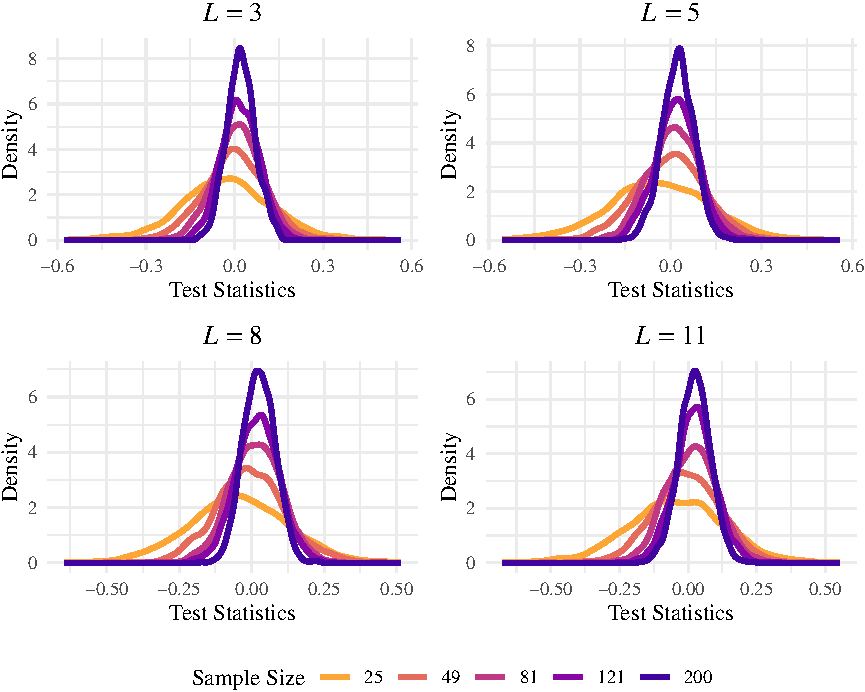
\includegraphics[width=0.8\linewidth]{../../Figures/PDF/Plot_density-1} 

}

\caption{Empirical densities obtained from $S_{\widetilde{H}_{\text{AO}}}(\bm{Z}; L)$ test under the null hypothesis.}\label{fig:Plot_density}
\end{figure}

Additionally, Table~\ref{tab:table_stat_combined} summarizes
the main descriptive statistics, including mean, standard
deviation~(SD), variance~(Var), skewness~(SK), excessive kurtosis~(EK)
and Anderson--Darling \(p\) values for normality. 


\setlength{\tabcolsep}{5pt}
\begin{table}[H]
\centering\centering\centering
\caption{\label{tab:table_stat_combined}Descriptive analysis of $S_{\widetilde{H}_{\text{AO}}}(\bm{Z}; L)$, with $L\in\left\{3,5, 8,11\right\}$ and $\mu=1$.}
\resizebox{\ifdim\width>\linewidth\linewidth\else\width\fi}{!}{
\footnotesize
\begin{tabu} to \linewidth {>{\centering}X>{\centering}X>{\raggedleft}X>{\raggedleft}X>{\raggedleft}X>{\raggedleft}X>{\raggedleft}X>{\raggedleft}X}
\toprule
\multicolumn{1}{c}{$\bm{L}$} & \multicolumn{1}{c}{$\bm{n}$} & \multicolumn{1}{c}{\textbf{Mean}} & \multicolumn{1}{c}{\textbf{SD}} & \multicolumn{1}{c}{\textbf{Var}} & \multicolumn{1}{c}{\textbf{SK}} & \multicolumn{1}{c}{\textbf{EK}} & \multicolumn{1}{c}{$p$-\textbf{value}}\\
\midrule
 & $25$ & $-0.0280$ & $\phantom{-}0.1547$ & $\phantom{-}0.0239$ & $-0.0076$ & $\phantom{-}0.4734$ & $\phantom{-}0.0022$\\

 & $49$ & $-0.0003$ & $\phantom{-}0.1053$ & $\phantom{-}0.0111$ & $-0.0562$ & $\phantom{-}0.2610$ & $\phantom{-}0.0582$\\

 & $81$ & $\phantom{-}0.0124$ & $\phantom{-}0.0796$ & $\phantom{-}0.0063$ & $-0.0124$ & $\phantom{-}0.0536$ & $\phantom{-}0.5278$\\

 & $121$ & $\phantom{-}0.0187$ & $\phantom{-}0.0630$ & $\phantom{-}0.0040$ & $\phantom{-}0.0337$ & $-0.1826$ & $\phantom{-}0.5894$\\

\multirow{-5}{*}[2\dimexpr\aboverulesep+\belowrulesep+\cmidrulewidth]{\centering\arraybackslash 3} & $200$ & $\phantom{-}0.0215$ & $\phantom{-}0.0490$ & $\phantom{-}0.0024$ & $\phantom{-}0.0625$ & $-0.0473$ & $\phantom{-}0.0860$\\
\cmidrule{1-8}
 & $25$ & $-0.0379$ & $\phantom{-}0.1669$ & $\phantom{-}0.0278$ & $\phantom{-}0.0007$ & $\phantom{-}0.1420$ & $\phantom{-}0.3267$\\

 & $49$ & $-0.0015$ & $\phantom{-}0.1150$ & $\phantom{-}0.0132$ & $-0.1025$ & $\phantom{-}0.1998$ & $\phantom{-}0.2582$\\

 & $81$ & $\phantom{-}0.0145$ & $\phantom{-}0.0869$ & $\phantom{-}0.0075$ & $\phantom{-}0.1008$ & $\phantom{-}0.5297$ & $\phantom{-}0.1121$\\

 & $121$ & $\phantom{-}0.0198$ & $\phantom{-}0.0687$ & $\phantom{-}0.0047$ & $\phantom{-}0.0127$ & $\phantom{-}0.0222$ & $\phantom{-}0.2919$\\

\multirow{-5}{*}[2\dimexpr\aboverulesep+\belowrulesep+\cmidrulewidth]{\centering\arraybackslash 5} & $200$ & $\phantom{-}0.0236$ & $\phantom{-}0.0529$ & $\phantom{-}0.0028$ & $-0.0467$ & $\phantom{-}0.0977$ & $\phantom{-}0.3346$\\
\cmidrule{1-8}
 & $25$ & $-0.0464$ & $\phantom{-}0.1680$ & $\phantom{-}0.0282$ & $-0.0121$ & $\phantom{-}0.0980$ & $\phantom{-}0.6477$\\

 & $49$ & $-0.0031$ & $\phantom{-}0.1202$ & $\phantom{-}0.0144$ & $\phantom{-}0.1282$ & $\phantom{-}0.2000$ & $\phantom{-}0.0038$\\

 & $81$ & $\phantom{-}0.0137$ & $\phantom{-}0.0883$ & $\phantom{-}0.0078$ & $-0.0279$ & $\phantom{-}0.2554$ & $\phantom{-}0.5567$\\

 & $121$ & $\phantom{-}0.0200$ & $\phantom{-}0.0738$ & $\phantom{-}0.0055$ & $-0.0089$ & $\phantom{-}0.0686$ & $\phantom{-}0.7502$\\

\multirow{-5}{*}[2\dimexpr\aboverulesep+\belowrulesep+\cmidrulewidth]{\centering\arraybackslash 8} & $200$ & $\phantom{-}0.0260$ & $\phantom{-}0.0546$ & $\phantom{-}0.0030$ & $\phantom{-}0.0716$ & $-0.0349$ & $\phantom{-}0.3771$\\
\cmidrule{1-8}
 & $25$ & $-0.0442$ & $\phantom{-}0.1735$ & $\phantom{-}0.0301$ & $-0.1422$ & $\phantom{-}0.2413$ & $\phantom{-}0.0981$\\

 & $49$ & $-0.0019$ & $\phantom{-}0.1201$ & $\phantom{-}0.0144$ & $-0.0503$ & $\phantom{-}0.1464$ & $\phantom{-}0.9576$\\

 & $81$ & $\phantom{-}0.0127$ & $\phantom{-}0.0917$ & $\phantom{-}0.0084$ & $-0.0172$ & $\phantom{-}0.0333$ & $\phantom{-}0.3179$\\

 & $121$ & $\phantom{-}0.0239$ & $\phantom{-}0.0729$ & $\phantom{-}0.0053$ & $-0.0127$ & $\phantom{-}0.2102$ & $\phantom{-}0.0596$\\

\multirow{-5}{*}[2\dimexpr\aboverulesep+\belowrulesep+\cmidrulewidth]{\centering\arraybackslash 11} & $200$ & $\phantom{-}0.0234$ & $\phantom{-}0.0572$ & $\phantom{-}0.0033$ & $-0.0233$ & $\phantom{-}0.1072$ & $\phantom{-}0.6740$\\
\bottomrule
\end{tabu}}
\end{table}
Results with \(p\) values greater than \(0.05\) do not indicate a violation of the
normality assumption. 
A low variance, skewness, and excessive kurtosis
of almost zero indicate limited dispersion, asymmetry, and a light tail.

Normal Q--Q plots confirm no evidence against a normal distribution, as
shown in Figure~\ref{fig:Plot_normality_qq}.
\begin{figure}[H]
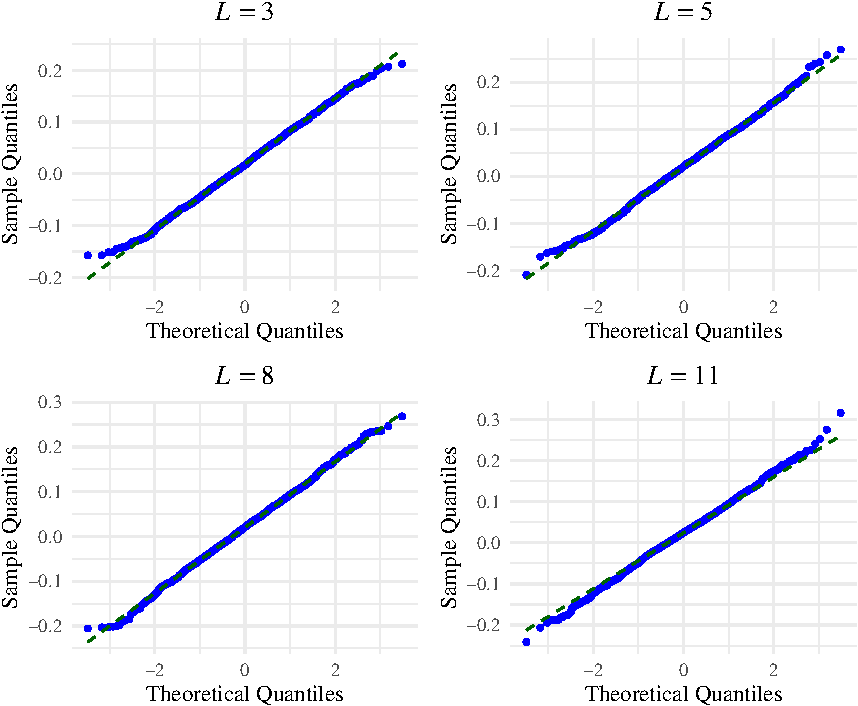
\includegraphics[width=0.9\linewidth]{../../Figures/PDF/Plot_normality_qq-1} \caption{Normal Q--Q plots for  $n=121$.}\label{fig:Plot_normality_qq}
\end{figure}

After checking the data's normality, we examined the proposed test's
abilities in terms of size and power. Under \(\mathcal{H}_0\), the
distribution of the test statistic is asymptotically normal. Therefore,
the \(p\) values are calculated as \(2\Phi(-|\varepsilon|)\), where
\(\Phi\) is the standard Gaussian cumulative distribution function, and
\(\varepsilon\) is the standardized test statistic given by: \[
\varepsilon=\frac{\widetilde{H}_{\text{AO}}(\bm{Z})-\left[H_{\Gamma_{\text{SAR}}}(L)+\ln \overline{\bm{Z}}\right]}{\widehat\sigma}.
\]

We have nominal levels of \SI{1}{\percent}, \SI{5}{\percent}, and
\SI{10}{\percent}. In terms of size, \(1000\) simulations were used for
different sample sizes from the \(\Gamma_{\text{SAR}}\) distribution,
with varying values of \(L\), and \(\mu=1\). In all cases, the nominal
level was achieved. We assessed the test power using \(1000\)
simulations for different sample sizes from the \(G_I^0\) distribution,
with \(\mu=1\), and \(\alpha=-2\). The power generally improves with
increasing sample size and number of looks. The results are shown in
Table~\ref{tab:table_size_power}.

\begin{table}[htb]
\centering\centering
\caption{\label{tab:table_size_power}Size and Power of the $S_{\widetilde{H}_{\text{AO}}}(\bm{Z})$ test statistic.}
\resizebox{\ifdim\width>\linewidth\linewidth\else\width\fi}{!}{
\begin{tabu} to \linewidth {>{\centering}X>{\centering}X>{\centering}X>{\centering}X>{\centering}X>{\centering}X>{\centering}X>{\centering}X}
\toprule
\multicolumn{1}{c}{ } & \multicolumn{1}{c}{ } & \multicolumn{3}{c}{Size} & \multicolumn{3}{c}{Power} \\
\cmidrule(l{3pt}r{3pt}){3-5} \cmidrule(l{3pt}r{3pt}){6-8}
\multicolumn{1}{c}{$\bm{L}$} & \multicolumn{1}{c}{$\bm{n}$} & \multicolumn{1}{c}{$\bm{1\%}$} & \multicolumn{1}{c}{$\bm{5\%}$} & \multicolumn{1}{c}{$\bm{10\%}$} & \multicolumn{1}{c}{$\bm{1\%}$} & \multicolumn{1}{c}{$\bm{5\%}$} & \multicolumn{1}{c}{$\bm{10\%}$}\\
\midrule
 & 25 & $\phantom{-}0.0160$ & $\phantom{-}0.0620$ & $\phantom{-}0.1070$ & $\phantom{-}0.6900$ & $\phantom{-}0.8450$ & $\phantom{-}0.8340$\\

 & 49 & $\phantom{-}0.0100$ & $\phantom{-}0.0480$ & $\phantom{-}0.0960$ & $\phantom{-}0.6890$ & $\phantom{-}0.8920$ & $\phantom{-}0.8480$\\

 & 81 & $\phantom{-}0.0120$ & $\phantom{-}0.0490$ & $\phantom{-}0.1080$ & $\phantom{-}0.6260$ & $\phantom{-}0.8750$ & $\phantom{-}0.8540$\\

\multirow{-4}{*}[1.5\dimexpr\aboverulesep+\belowrulesep+\cmidrulewidth]{\centering\arraybackslash 3} & 121 & $\phantom{-}0.0090$ & $\phantom{-}0.0690$ & $\phantom{-}0.1190$ & $\phantom{-}0.5680$ & $\phantom{-}0.8620$ & $\phantom{-}0.8230$\\
\cmidrule{1-8}
 & 25 & $\phantom{-}0.0210$ & $\phantom{-}0.0660$ & $\phantom{-}0.1130$ & $\phantom{-}0.9120$ & $\phantom{-}0.9620$ & $\phantom{-}0.9880$\\

 & 49 & $\phantom{-}0.0100$ & $\phantom{-}0.0460$ & $\phantom{-}0.1080$ & $\phantom{-}0.9470$ & $\phantom{-}0.9820$ & $\phantom{-}0.9960$\\

 & 81 & $\phantom{-}0.0120$ & $\phantom{-}0.0560$ & $\phantom{-}0.1070$ & $\phantom{-}0.9580$ & $\phantom{-}0.9900$ & $\phantom{-}0.9960$\\

\multirow{-4}{*}[1.5\dimexpr\aboverulesep+\belowrulesep+\cmidrulewidth]{\centering\arraybackslash 5} & 121 & $\phantom{-}0.0150$ & $\phantom{-}0.0640$ & $\phantom{-}0.1150$ & $\phantom{-}0.9420$ & $\phantom{-}0.9780$ & $\phantom{-}0.9950$\\
\cmidrule{1-8}
 & 25 & $\phantom{-}0.0210$ & $\phantom{-}0.0650$ & $\phantom{-}0.1080$ & $\phantom{-}0.9930$ & $\phantom{-}0.9950$ & $\phantom{-}0.9970$\\

 & 49 & $\phantom{-}0.0060$ & $\phantom{-}0.0470$ & $\phantom{-}0.0860$ & $\phantom{-}0.9980$ & $\phantom{-}1.0000$ & $\phantom{-}0.9970$\\

 & 81 & $\phantom{-}0.0120$ & $\phantom{-}0.0490$ & $\phantom{-}0.1000$ & $\phantom{-}0.9930$ & $\phantom{-}0.9980$ & $\phantom{-}0.9990$\\

\multirow{-4}{*}[1.5\dimexpr\aboverulesep+\belowrulesep+\cmidrulewidth]{\centering\arraybackslash 8} & 121 & $\phantom{-}0.0150$ & $\phantom{-}0.0650$ & $\phantom{-}0.1220$ & $\phantom{-}0.9970$ & $\phantom{-}0.9990$ & $\phantom{-}0.9980$\\
\cmidrule{1-8}
 & 25 & $\phantom{-}0.0130$ & $\phantom{-}0.0610$ & $\phantom{-}0.1000$ & $\phantom{-}0.9990$ & $\phantom{-}0.9990$ & $\phantom{-}0.9990$\\

 & 49 & $\phantom{-}0.0100$ & $\phantom{-}0.0450$ & $\phantom{-}0.0920$ & $\phantom{-}0.9980$ & $\phantom{-}0.9990$ & $\phantom{-}0.9990$\\

 & 81 & $\phantom{-}0.0170$ & $\phantom{-}0.0530$ & $\phantom{-}0.1050$ & $\phantom{-}1.0000$ & $\phantom{-}1.0000$ & $\phantom{-}1.0000$\\

\multirow{-4}{*}[1.5\dimexpr\aboverulesep+\belowrulesep+\cmidrulewidth]{\centering\arraybackslash 11} & 121 & $\phantom{-}0.0160$ & $\phantom{-}0.0680$ & $\phantom{-}0.1180$ & $\phantom{-}0.9980$ & $\phantom{-}1.0000$ & $\phantom{-}0.9980$\\
\bottomrule
\end{tabu}}
\end{table}

\subsection[The Proposed Test Based on CV and a Robust Alternative]{The Proposed Test Based on Coefficient of Variation and a
Robust
Alternative}\label{the-proposed-test-based-on-coefficient-of-variation-and-a-robust-alternative}

In addition to the \(S_{\widetilde{H}_{\text{AO}}}(\bm{Z}; L)\) test, we
also propose a test statistic based on the classical CV. This test
statistic is defined as follows: \begin{align}
    T_{\text{CV}}=\frac{S}{\overline{Z}},
\end{align} where \(S\) and \(\overline{Z}\) are the sample standard
deviation and mean, respectively.

Similarly, we use another test statistic based on the ratio of the MnAD
to the median. This statistic is given by: \begin{align}
    T_{\text{CV}_{\text{MnAD}}}=\frac{\text{MnAD}}{\text{Median}}.
\end{align}

We proceed to identify suitable models for these estimators of the CV,
and then form test statistics.

The situations in which the use of CV and \(\text{CV}_{\text{MnAD}}\)
may be appropriate, i.e., when the observations are positive, the
log-normal (LN) and the inverse Gaussian distribution (IG) are often
more appropriate than the Gamma and Weibull
distributions~\citep{Chaubey2017,takagi1997application}.

It is shown that the IG distribution is well approximated by the
log-normal distribution, which means that the IG distribution also does
not share the problem of the non-existence of a fixed-width confidence
interval with the Gaussian case~\citep{whitmore1978}.

The biparametric LN distribution has density:

\begin{align}
    f_Z(z;\mu_{\text{LN}}, \sigma_{\text{LN}} )=\frac{1}{\sigma_{\text{LN}} z\sqrt{2\pi}}\exp\left\{-\frac{(\ln z- \mu_{\text{LN}})^2}{2\sigma_{\text{LN}}^2}\right\}\mathbbm 1_{\mathbbm R_+}(z),
\end{align}\\
with \(\mu_{\text{LN}}\) is any real number, and \(\sigma_{\text{LN}}\)
is positive.

\subsection{Model Selection Criterion}\label{model-selection-criterion}

We used the Akaike information criterion (AIC) and the Bayesian
information criterion (BIC) to select the best-fitting distribution.

The AIC deals with the trade-off between the goodness-of-fit and the
model's simplicity in terms of the number of model
parameters~\citep{Burnham2004}. The model or distribution with the lowest
value of AIC is chosen to be the best. The BIC assesses goodness-of-fit
of a distribution or model, but avoids overfitting by penalising
additional degrees of freedom~\citep{Dziak2019}. The model with the
lowest BIC value is chosen as the best.

The AIC and BIC results in
Tables~\ref{tab:table_aic_gamma}--\ref{tab:table_aic_gio_MnADmedian}
indicate that the CV and \(\text{CV}_{\text{MnAD}}\) data from different
distributed \(\Gamma_{\text{SAR}}\) and \(G_I^0\) synthetic sample sizes
match the properties of an LN distribution. It is important to note that
this conclusion was drawn empirically based on a dictionary of
analytically tractable distributions and well-defined under
biparametric, unimodal, asymmetric, and positive distributions.

Figures~\ref{fig:Plot_cv}--\ref{fig:Plot_madmed_gi0_MnADmedian} show
empirical and fitted density plots, Q--Q plots, P--P plots, as well as
empirical and fitted cumulative distribution functions. They provide
qualitative sources that confirm that the LN distribution is the most
appropriate distribution. As expected, both test statistics work well
under the null hypothesis. Under the alternative hypothesis, the P--P
plot shows that \(\text{CV}_{\text{MnAD}}\) is more robust than CV,
although both statistics suffer from the tail effect caused by the
distributed \(G_I^0\) data.

\begin{table}[H]
\centering\centering
\caption{\label{tab:table_aic_gamma}AIC and BIC values for evaluating the best distribution with CV data from $\Gamma_{\text{SAR}}$.}
\resizebox{\ifdim\width>\linewidth\linewidth\else\width\fi}{!}{
\begin{tabu} to \linewidth {>{\centering}X>{\centering}X>{\centering}X>{\centering}X>{\raggedleft}X>{\raggedleft}X>{\raggedleft}X}
\toprule
\multicolumn{1}{c}{\textbf{Criterion}} & \multicolumn{1}{c}{$\bm{n}$} & \multicolumn{1}{c}{\textbf{Normal}} & \multicolumn{1}{c}{\textbf{Lognormal}} & \multicolumn{1}{c}{\textbf{Gamma}} & \multicolumn{1}{c}{\textbf{Weibull}} & \multicolumn{1}{c}{\textbf{Inverse Gaussian}}\\
\midrule
 & $25$ & $-38031.9$ & $-38266.7$ & $-38311.8$ & $-36413.2$ & $-38261.6$\\

 & $49$ & $-47698.2$ & $-47913.7$ & $-47905.6$ & $-45554.0$ & $-47911.6$\\

 & $81$ & $-55382.1$ & $-55494.7$ & $-55494.9$ & $-53220.4$ & $-55493.8$\\

\multirow{-4}{*}[1.5\dimexpr\aboverulesep+\belowrulesep+\cmidrulewidth]{\centering\arraybackslash AIC} & $121$ & $-61344.9$ & $-61470.8$ & $-61453.8$ & $-58876.0$ & $-61470.5$\\
\cmidrule{1-7}
 & $25$ & $-38016.7$ & $-38251.5$ & $-38296.6$ & $-36398.0$ & $-38246.4$\\

 & $49$ & $-47683.0$ & $-47898.5$ & $-47890.4$ & $-45538.7$ & $-47896.4$\\

 & $81$ & $-55366.9$ & $-55479.5$ & $-55479.6$ & $-53205.2$ & $-55478.6$\\

\multirow{-4}{*}[1.5\dimexpr\aboverulesep+\belowrulesep+\cmidrulewidth]{\centering\arraybackslash BIC} & $121$ & $-61329.7$ & $-61455.6$ & $-61438.6$ & $-58860.8$ & $-61455.2$\\
\bottomrule
\end{tabu}}
\end{table}

\begin{table}[H]
\centering\centering
\caption{\label{tab:table_aic}AIC and BIC values for evaluating the best distribution with CV data from $G_I^0$.}
\resizebox{\ifdim\width>\linewidth\linewidth\else\width\fi}{!}{
\begin{tabu} to \linewidth {>{\centering}X>{\centering}X>{\centering}X>{\centering}X>{\centering}X>{\centering}X>{\centering}X}
\toprule
\multicolumn{1}{c}{\textbf{Criterion}} & \multicolumn{1}{c}{$\bm{n}$} & \multicolumn{1}{c}{\textbf{Normal}} & \multicolumn{1}{c}{\textbf{Lognormal}} & \multicolumn{1}{c}{\textbf{Gamma}} & \multicolumn{1}{c}{\textbf{Weibull}} & \multicolumn{1}{c}{\textbf{Inverse Gaussian}}\\
\midrule
 & $25$ & $\phantom{-}8254.04$ & $\phantom{-}2186.31$ & $\phantom{-}3628.40$ & $\phantom{-}8383.58$ & $\phantom{-}2257.63$\\

 & $49$ & $\phantom{-}8821.79$ & $\phantom{-}1689.03$ & $\phantom{-}3483.10$ & $\phantom{-}9533.53$ & $\phantom{-}1835.29$\\

 & $81$ & $\phantom{-}8525.81$ & $\phantom{-}866.29$ & $\phantom{-}2853.31$ & $\phantom{-}9822.48$ & $\phantom{-}1057.91$\\

\multirow{-4}{*}[1.5\dimexpr\aboverulesep+\belowrulesep+\cmidrulewidth]{\centering\arraybackslash AIC} & $121$ & $\phantom{-}8708.81$ & $\phantom{-}131.86$ & $\phantom{-}2341.06$ & $\phantom{-}10506.49$ & $\phantom{-}398.53$\\
\cmidrule{1-7}
 & $25$ & $\phantom{-}8269.27$ & $\phantom{-}2201.54$ & $\phantom{-}3643.63$ & $\phantom{-}8398.81$ & $\phantom{-}2272.86$\\

 & $49$ & $\phantom{-}8837.02$ & $\phantom{-}1704.26$ & $\phantom{-}3498.33$ & $\phantom{-}9548.76$ & $\phantom{-}1850.52$\\

 & $81$ & $\phantom{-}8541.04$ & $\phantom{-}881.52$ & $\phantom{-}2868.55$ & $\phantom{-}9837.72$ & $\phantom{-}1073.14$\\

\multirow{-4}{*}[1.5\dimexpr\aboverulesep+\belowrulesep+\cmidrulewidth]{\centering\arraybackslash BIC} & $121$ & $\phantom{-}8724.04$ & $\phantom{-}147.09$ & $\phantom{-}2356.29$ & $\phantom{-}10521.72$ & $\phantom{-}413.76$\\
\bottomrule
\end{tabu}}
\end{table}

\begin{table}[H]
\centering\centering
\caption{\label{tab:table_aic_gamma_madmed}AIC and BIC values for evaluating the best distribution with $\text{CV}_{\text{MnAD}}$ data from $\Gamma_{\text{SAR}}$.}
\resizebox{\ifdim\width>\linewidth\linewidth\else\width\fi}{!}{
\begin{tabu} to \linewidth {>{\centering}X>{\centering}X>{\centering}X>{\centering}X>{\centering}X>{\centering}X>{\centering}X}
\toprule
\multicolumn{1}{c}{\textbf{Criterion}} & \multicolumn{1}{c}{$\bm{n}$} & \multicolumn{1}{c}{\textbf{Normal}} & \multicolumn{1}{c}{\textbf{Lognormal}} & \multicolumn{1}{c}{\textbf{Gamma}} & \multicolumn{1}{c}{\textbf{Weibull}} & \multicolumn{1}{c}{\textbf{Inverse Gaussian}}\\
\midrule
 & $25$ & $-38375.56$ & $-39147.85$ & $-39066.29$ & $-36652.49$ & $-39143.61$\\

 & $49$ & $-48386.11$ & $-48795.32$ & $-48745.48$ & $-46240.91$ & $-48793.83$\\

 & $81$ & $-56072.87$ & $-56322.32$ & $-56290.02$ & $-53836.04$ & $-56322.12$\\

\multirow{-4}{*}[1.5\dimexpr\aboverulesep+\belowrulesep+\cmidrulewidth]{\centering\arraybackslash AIC} & $121$ & $-62217.14$ & $-62394.77$ & $-62369.32$ & $-59861.80$ & $-62394.57$\\
\cmidrule{1-7}
 & $25$ & $-38360.32$ & $-39132.62$ & $-39051.05$ & $-36637.26$ & $-39128.38$\\

 & $49$ & $-48370.87$ & $-48780.09$ & $-48730.25$ & $-46225.67$ & $-48778.60$\\

 & $81$ & $-56057.64$ & $-56307.09$ & $-56274.79$ & $-53820.81$ & $-56306.89$\\

\multirow{-4}{*}[1.5\dimexpr\aboverulesep+\belowrulesep+\cmidrulewidth]{\centering\arraybackslash BIC} & $121$ & $-62201.91$ & $-62379.54$ & $-62354.09$ & $-59846.56$ & $-62379.33$\\
\bottomrule
\end{tabu}}
\end{table}

\begin{table}[H]
\centering\centering
\caption{\label{tab:table_aic_gio_MnADmedian}AIC and BIC values for evaluating the best distribution with $\text{CV}_{\text{MnAD}}$ data from $G_I^0$.}
\resizebox{\ifdim\width>\linewidth\linewidth\else\width\fi}{!}{
\begin{tabu} to \linewidth {>{\centering}X>{\centering}X>{\centering}X>{\centering}X>{\centering}X>{\centering}X>{\centering}X}
\toprule
\multicolumn{1}{c}{\textbf{Criterion}} & \multicolumn{1}{c}{$\bm{n}$} & \multicolumn{1}{c}{\textbf{Normal}} & \multicolumn{1}{c}{\textbf{Lognormal}} & \multicolumn{1}{c}{\textbf{Gamma}} & \multicolumn{1}{c}{\textbf{Weibull}} & \multicolumn{1}{c}{\textbf{Inverse Gaussian}}\\
\midrule
 & $25$ & $-13302.39$ & $-15575.23$ & $-15158.42$ & $-11933.35$ & $-15565.03$\\

 & $49$ & $-23265.27$ & $-24529.72$ & $-24284.47$ & $-20986.94$ & $-24522.28$\\

 & $81$ & $-29908.19$ & $-30960.38$ & $-30747.90$ & $-25233.41$ & $-30946.54$\\

\multirow{-4}{*}[1.5\dimexpr\aboverulesep+\belowrulesep+\cmidrulewidth]{\centering\arraybackslash AIC} & $121$ & $-36496.78$ & $-37128.07$ & $-36991.41$ & $-32366.52$ & $-37123.20$\\
\cmidrule{1-7}
 & $25$ & $-13287.16$ & $-15559.99$ & $-15143.19$ & $-11918.12$ & $-15549.80$\\

 & $49$ & $-23250.04$ & $-24514.48$ & $-24269.24$ & $-20971.71$ & $-24507.05$\\

 & $81$ & $-29892.96$ & $-30945.15$ & $-30732.67$ & $-25218.17$ & $-30931.31$\\

\multirow{-4}{*}[1.5\dimexpr\aboverulesep+\belowrulesep+\cmidrulewidth]{\centering\arraybackslash BIC} & $121$ & $-36481.55$ & $-37112.84$ & $-36976.18$ & $-32351.28$ & $-37107.97$\\
\bottomrule
\end{tabu}}
\end{table}

\begin{figure}[H]

{\centering 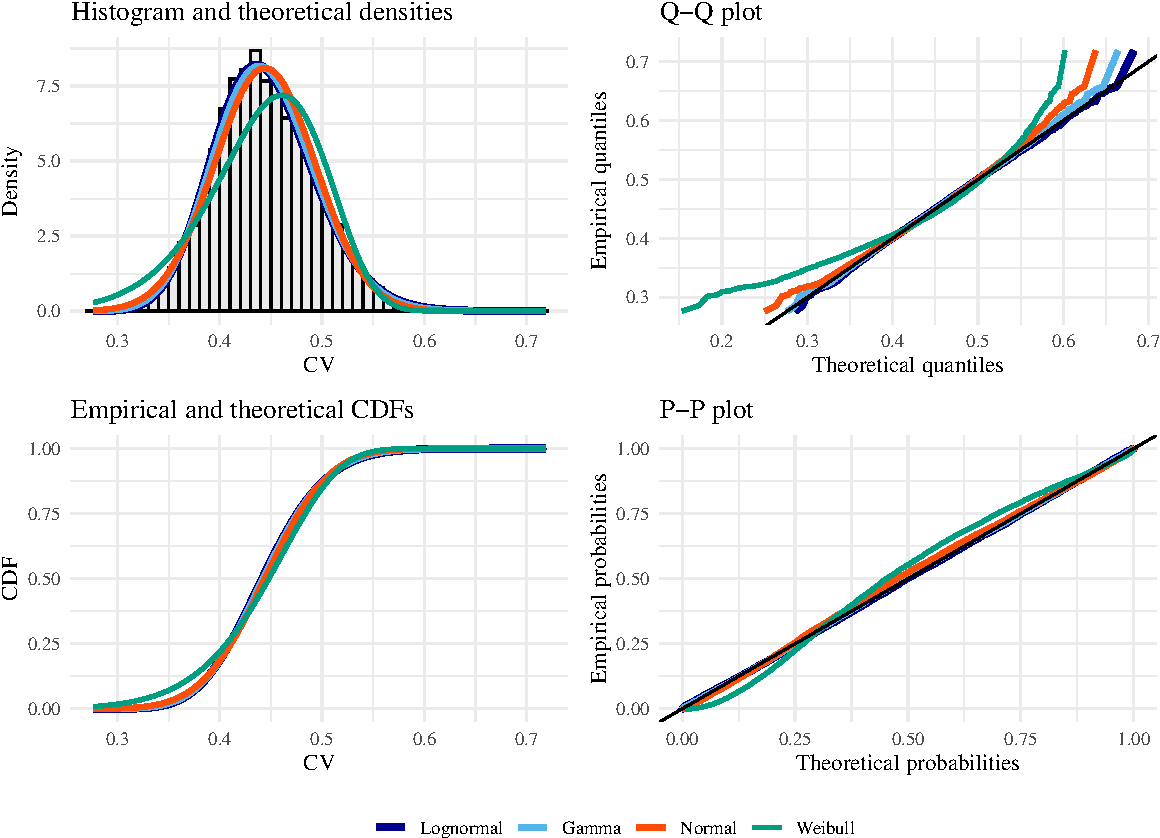
\includegraphics[width=0.8\linewidth]{../../Figures/PDF/Plot_cv_gamma-1} 

}

\caption{Goodness of fit plots for evaluating the best distribution with CV data from $\Gamma_{\text{SAR}}$ (under the null hypothesis), with $n=49$, $L=5$, and $\mu=1$.}\label{fig:Plot_cv_gamma}
\end{figure}

\begin{figure}[H]

{\centering 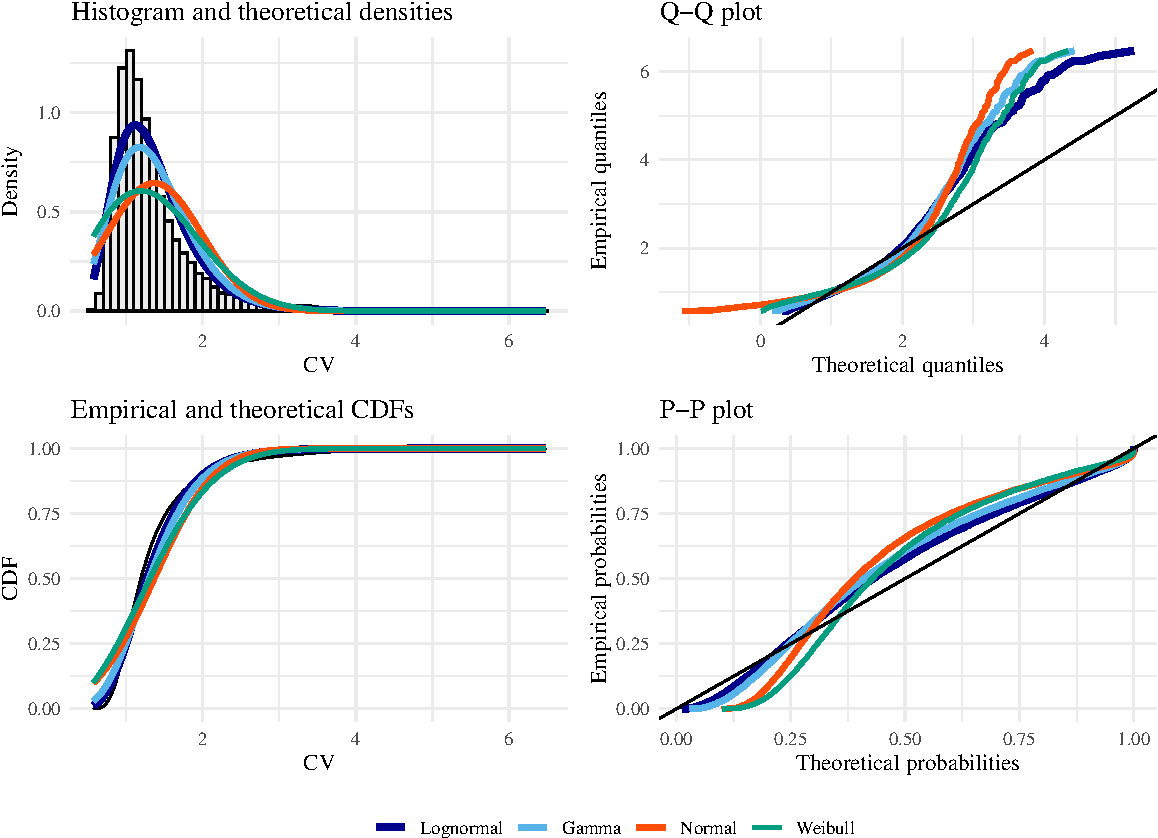
\includegraphics[width=0.8\linewidth]{../../Figures/PDF/Plot_cv-1} 

}

\caption{Goodness of fit plots for evaluating the best distribution with $\text{CV}$ data from $G_I^0$ (under the alternative hypothesis), with  $n=49$, $L=5$, $\mu=1$, and $\alpha=-3$.}\label{fig:Plot_cv}
\end{figure}

\begin{figure}[H]

{\centering 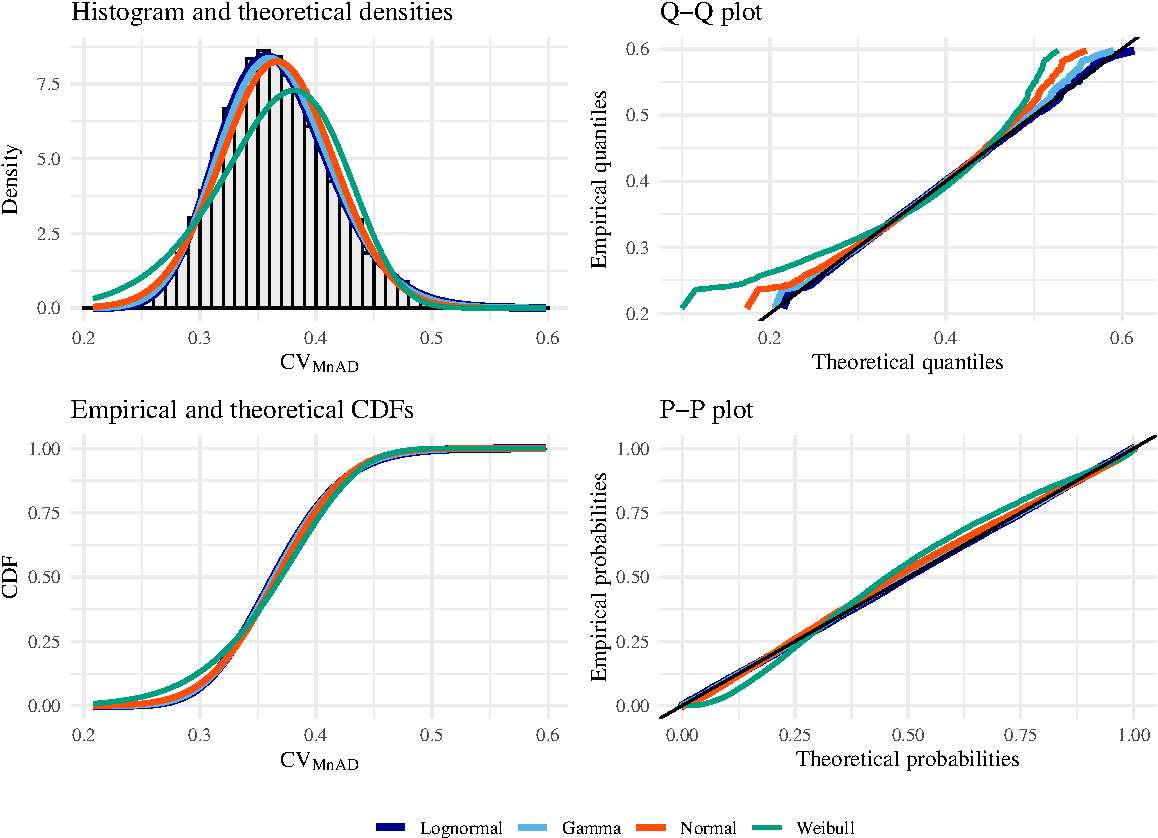
\includegraphics[width=0.8\linewidth]{../../Figures/PDF/Plot_MnADmedian_gamma-1} 

}

\caption{Goodness of fit plots for evaluating the best distribution with $\text{CV}_{\text{MnAD}}$ data from $\Gamma_{\text{SAR}}$ (under the null hypothesis), with  $n=49$, $L=5$, and $\mu=1$.}\label{fig:Plot_MnADmedian_gamma}
\end{figure}
\begin{figure}[H]

{\centering 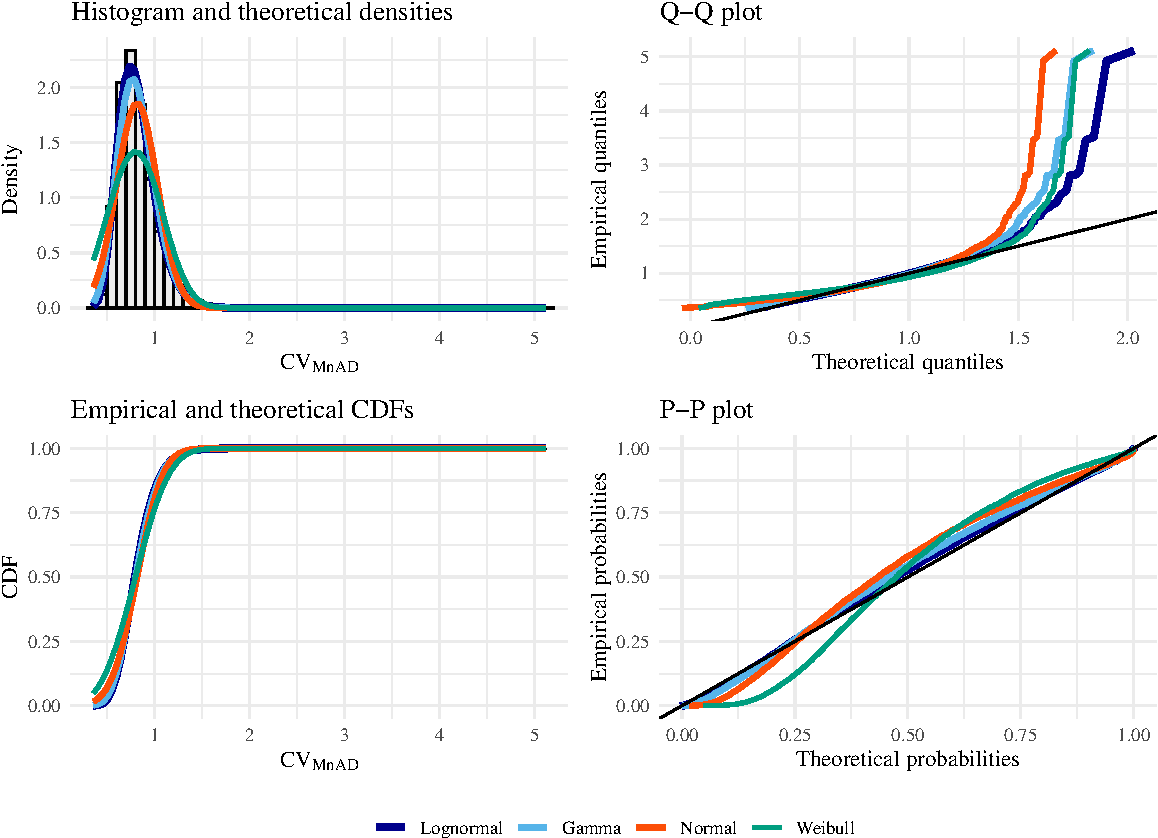
\includegraphics[width=0.8\linewidth]{../../Figures/PDF/Plot_madmed_gi0_MnADmedian-1} 

}

\caption{Goodness of fit plots for evaluating the best distribution with $CV_{\text{MnAD}}$ data from $G_I^0$ (under the alternative hypothesis), with  $n=49$, $L=5$, $\mu=1$, and $\alpha=-3$.}\label{fig:Plot_madmed_gi0_MnADmedian}
\end{figure}

%\begin{figure}[hbt]
%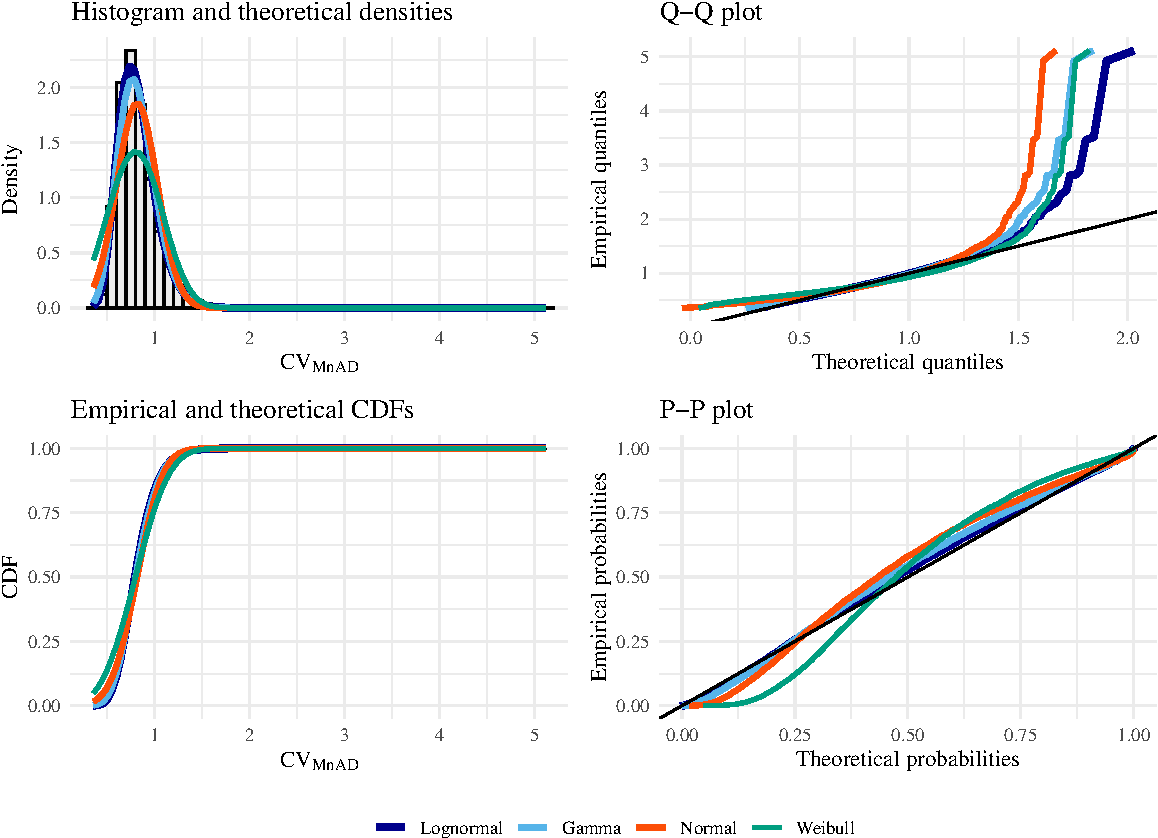
\includegraphics[width=0.8\linewidth]{../../Figures/PDF/Plot_madmed_gi0_MnADmedian-1} \caption{Goodness of fit plots for evaluating the best distribution with $CV_{\text{MnAD}}$ data from $G_I^0$ (under the alternative hypothesis), with  $n=49$, $L=5$, $\mu=1$, and $\alpha=-3$.}\label{fig:Plot_madmed_gi0_MnADmedian}
%\end{figure}
\chapter{Results}\label{chp:results}
%\section{Results}\label{sec:Results}

This section presents the simulations we performed to evaluate the
proposed test statistics' performance, followed by applications to SAR
data.

\subsection{Simulated Data}\label{simulated-data}

Figure~\ref{fig:sim_Phantom} \ref{fig:sim_Phantom_1} shows the phantom with dimensions of
\(500\times500\) pixels.
 It was proposed by~\citet{Gomez2017} as a tool
to assess the performance of speckle-reduction filters.

Figure~\ref{fig:sim_Phantom} \ref{fig:sim_Phantom_2} shows the simulated image, where each
small phantom displaying texture variations. The observations are
independent draws from the \(G^0_I\) distribution~\eqref{E:gi02}, with
\(L = 5\) and varying \(\alpha\) and \(\mu\), annotated in the image for
each quadrant. 
Light regions correspond to textured observations
(heterogeneous), while darker regions represent textureless areas
(homogeneous).
\begin{figure}[H]
  \centering
  \begin{subfigure}[b]{0.38\textwidth}
    \centering
    
\includegraphics[width=60mm]{../../Figures/PNG/Phantom1}
    \caption{Phantom.}
    \label{fig:sim_Phantom_1}
  \end{subfigure}
  \hfill
  \begin{subfigure}[b]{0.58\textwidth}
    \centering
    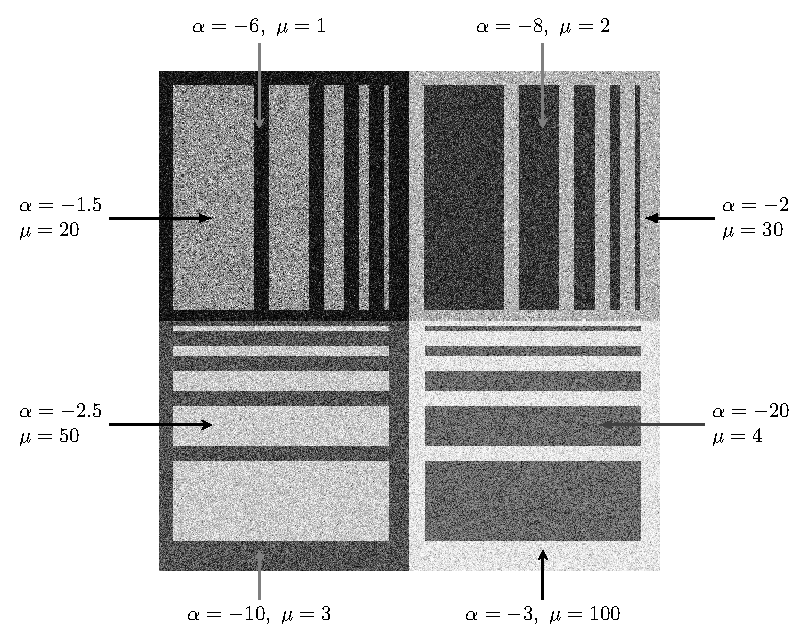
\includegraphics[width=80mm]{../../Figures/PNG/Phantom_label/Phantom_labels}
    \caption{Simulated image, varying $\alpha$ and $\mu$, with $L=5$.}
    \label{fig:sim_Phantom_2}
  \end{subfigure}
  \caption{Synthetic dataset.}
  \label{fig:sim_Phantom}
\end{figure}


The \(\alpha\) parameter of the \(G_I^0\) distribution is essential for
interpreting texture characteristics. Values near zero greater than
\(-3\) suggest extremely textured targets, such as urban
zones~\citep{Frery2019a}. 
As the value decreases, it indicates regions with moderate texture (in the \(\left[-6,-3\right]\) region), related to
forest zones, while values below \(-6\) correspond to textureless
regions, such as pasture, agricultural fields, and water
bodies~\citep{Neto2023}.




We applied the three test statistics, namely
\(S_{\widetilde{H}_{\text{AO}}}(\bm{Z}; L)\), \(T_\text{CV}\), and
\(T_{\text{CV}_{\text{MnAD}}}\), to the simulated image using local
sliding windows of size \(7\times 7\), as shown in
Figures~\ref{fig:sim_results} \ref{fig:sim_results-1}--\ref{fig:sim_results-3}.
\begin{figure}[H]
  \centering
  \begin{subfigure}[b]{0.3\textwidth}
    \centering
    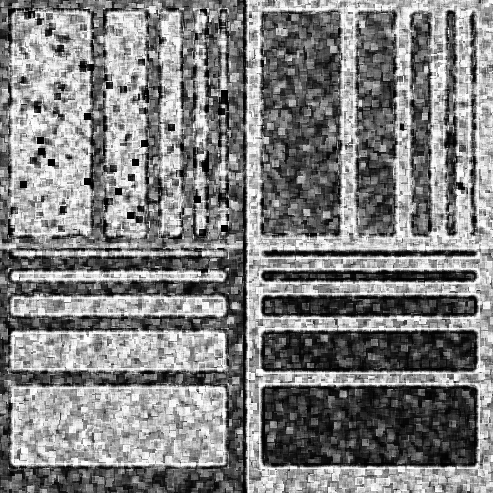
\includegraphics[width=\textwidth]{../../Figures/PNG/Entropy_Phantom_4_z1_200}
    \caption{$S_{\widetilde{H}_{\text{AO}}}(\bm{Z}; L)$}
    \label{fig:sim_results-1}
  \end{subfigure}
  \hfill
  \begin{subfigure}[b]{0.3\textwidth}
    \centering
    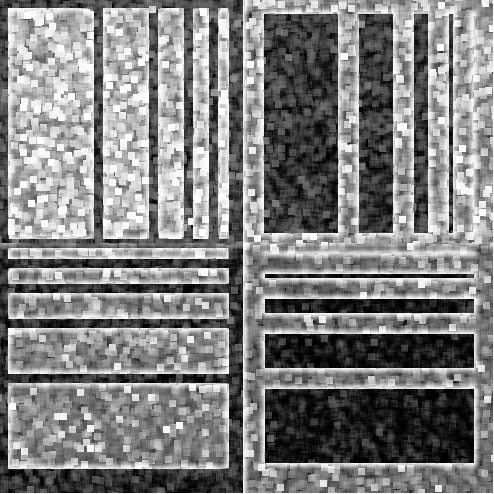
\includegraphics[width=\textwidth]{../../Figures/PNG/cv_Phantom_4_z1}
    \caption{$T_\text{CV}$}
    \label{fig:sim_results-2}
  \end{subfigure}
  \hfill
  \begin{subfigure}[b]{0.3\textwidth}
    \centering
    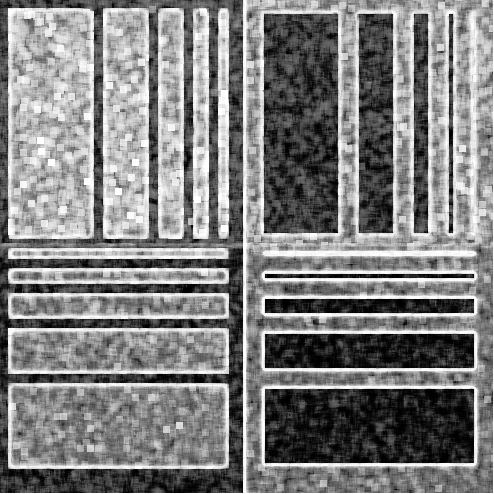
\includegraphics[width=\textwidth]{../../Figures/PNG/mnad_Phantom_z1}
    \caption{$T_{\text{CV}_{\text{MnAD}}}$}
    \label{fig:sim_results-3}
  \end{subfigure}
  \caption{Results of applying the test statistics to the simulated image.}
  \label{fig:sim_results}
\end{figure}



The resulting \(p\)-values for each test are shown in
Figures~\ref{fig:sim_SAR_Images} \ref{fig:sim_SAR_Images-1}--\ref{fig:sim_SAR_Images-3}. In
Figures~\ref{fig:sim_SAR_Images_p05} \ref{fig:sim_SAR_Images_p05-1}--\ref{fig:sim_SAR_Images_p05-3}, maps are depicted using a
color table between black, gray levels, and white. All \(p\)-values
above \(0.05\) are represented in white (indicating no evidence to
reject the null hypothesis), while those below \(0.05\) are shown in
black (indicating evidence to reject the hypothesis). 
We notice that the \(S_{\widetilde{H}_{\text{AO}}}(\bm{Z}; L)\) performs significantly
better than the other tests in identifying heterogeneous areas in the
simulated image.

\begin{figure}[H]
  \centering
  \begin{subfigure}[b]{0.3\textwidth}
    \centering
    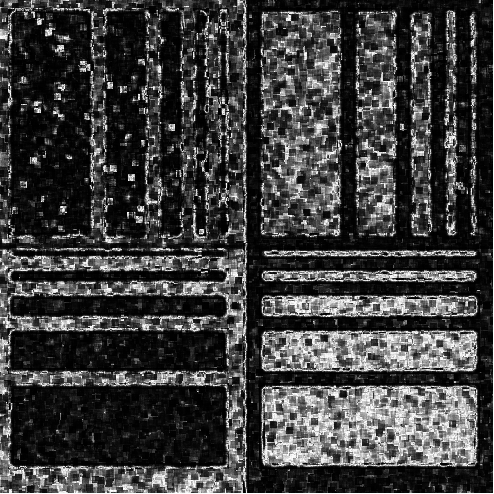
\includegraphics[width=\textwidth]{../../Figures/PNG/H_pvalue_Phantom_4_z1_200b}
    \caption{$S_{\widetilde{H}_{\text{AO}}}(\bm{Z}; L)$}
    \label{fig:sim_SAR_Images-1}
  \end{subfigure}
  \hfill
  \begin{subfigure}[b]{0.3\textwidth}
    \centering
    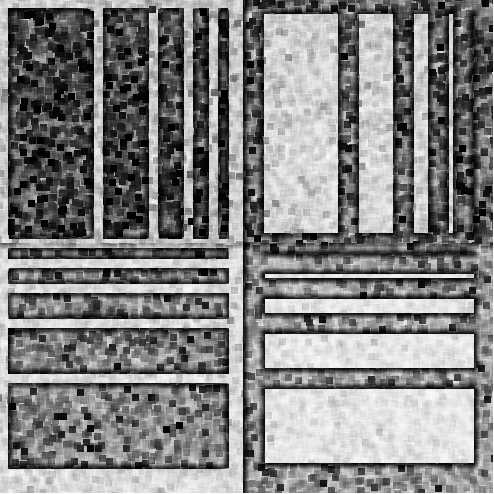
\includegraphics[width=\textwidth]{../../Figures/PNG/cv_pvalues_Phantom_4_z1}
    \caption{$T_\text{CV}$}
    \label{fig:sim_SAR_Images-2}
  \end{subfigure}
  \hfill
  \begin{subfigure}[b]{0.3\textwidth}
    \centering
    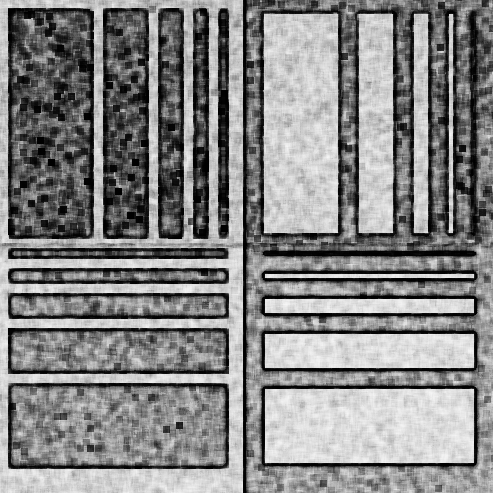
\includegraphics[width=\textwidth]{../../Figures/PNG/mnad_p_values_Phantom_mnad_7_z1}
     \caption{$T_{\text{CV}_{\text{MnAD}}}$}
    \label{fig:sim_SAR_Images-3}
  \end{subfigure}
  \caption{Map of $p$-values of simulated image for each test. }
  \label{fig:sim_SAR_Images}
\end{figure}



\begin{figure}[H]
  \centering
  \begin{subfigure}[b]{0.3\textwidth}
    \centering
    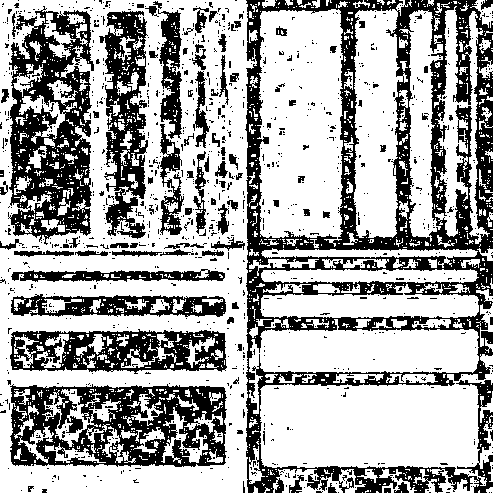
\includegraphics[width=\textwidth]{../../Figures/PNG/H_005_Phantom_4_z1_AO_200b}
    \caption{$S_{\widetilde{H}_{\text{AO}}}(\bm{Z}; L)$}
    \label{fig:sim_SAR_Images_p05-1}
  \end{subfigure}
  \hfill
  \begin{subfigure}[b]{0.3\textwidth}
    \centering
    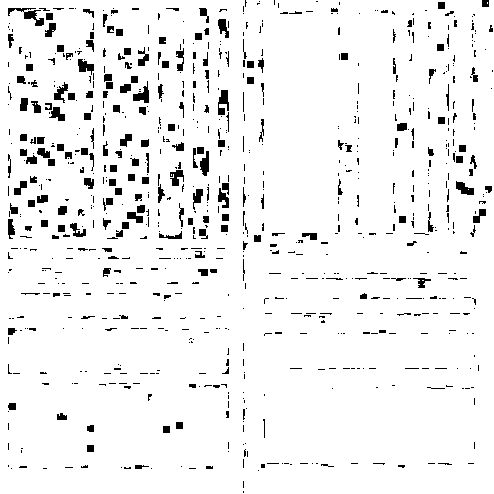
\includegraphics[width=\textwidth]{../../Figures/PNG/cv_005_pvalues_Phantom_4_z1}
    \caption{$T_\text{CV}$}
    \label{fig:sim_SAR_Images_p05-2}
  \end{subfigure}
  \hfill
  \begin{subfigure}[b]{0.3\textwidth}
    \centering
    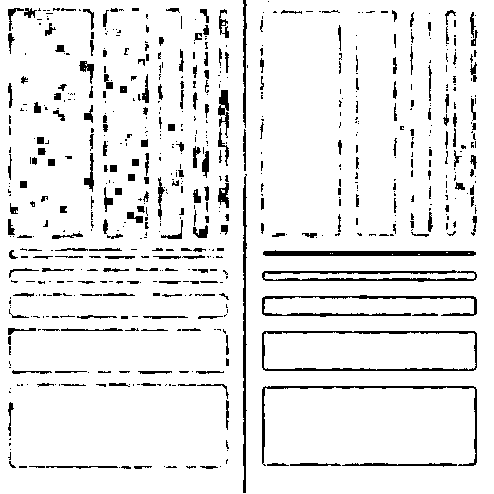
\includegraphics[width=\textwidth]{../../Figures/PNG/mnad_005_Phantom_7_z1}
     \caption{$T_{\text{CV}_{\text{MnAD}}}$}
    \label{fig:sim_SAR_Images_p05-3}
  \end{subfigure}
  \caption{Results for a threshold of $0.05$ of the $p$-value of simulated image for each test. }
  \label{fig:sim_SAR_Images_p05}
\end{figure}




\subsection{SAR Data}\label{sar-data}

We evaluated the proposed test statistics using three SAR images: one of
the coast of Jalisco, Mexico (with a spatial resolution of 20 m both
along azimuth and range directions) and two of Illinois, USA (with a
spatial resolution of \SI{10}{\meter} both along azimuth and range
directions), acquired by the Sentinel-1B satellite operating in C-band,
with VV polarization and intensity format. 
The first two images have a size of \(512 \times 512\) pixels, while the third has
\(1024 \times 1024\) pixels, and they contain mountainous areas,
agricultural regions, water bodies, and urban areas, as shown in
Figures~\ref{fig:real_SAR_Images_coe} \ref{fig:real_SAR_Images_coe-1}--\ref{fig:real_SAR_Images_coe-3}.

\begin{figure}[H]
  \centering
  \begin{subfigure}[b]{0.3\textwidth}
    \centering
    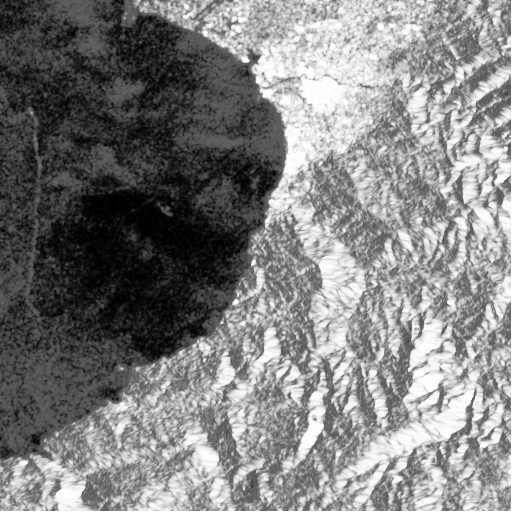
\includegraphics[width=\textwidth]{../../Figures/PNG/Mexico_512}
    \caption{Coast of Jalisco, $L=18$}
    \label{fig:real_SAR_Images_coe-1}
  \end{subfigure}
  \hfill
  \begin{subfigure}[b]{0.3\textwidth}
    \centering
    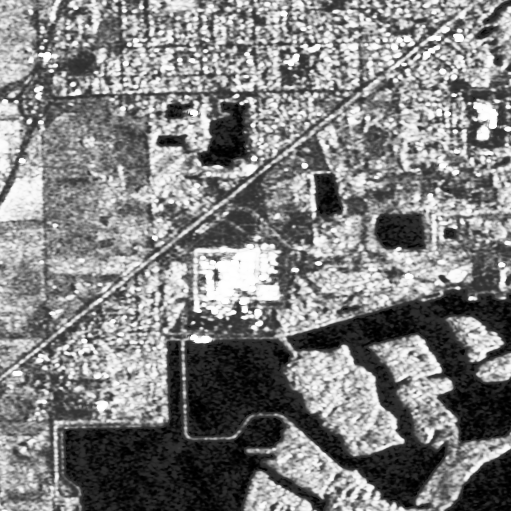
\includegraphics[width=\textwidth]{../../Figures/PNG/lake_512}
    \caption{Illinois-Region 1, $L=36$}
    \label{fig:real_SAR_Images_coe-2}
  \end{subfigure}
  \hfill
  \begin{subfigure}[b]{0.3\textwidth}
    \centering
    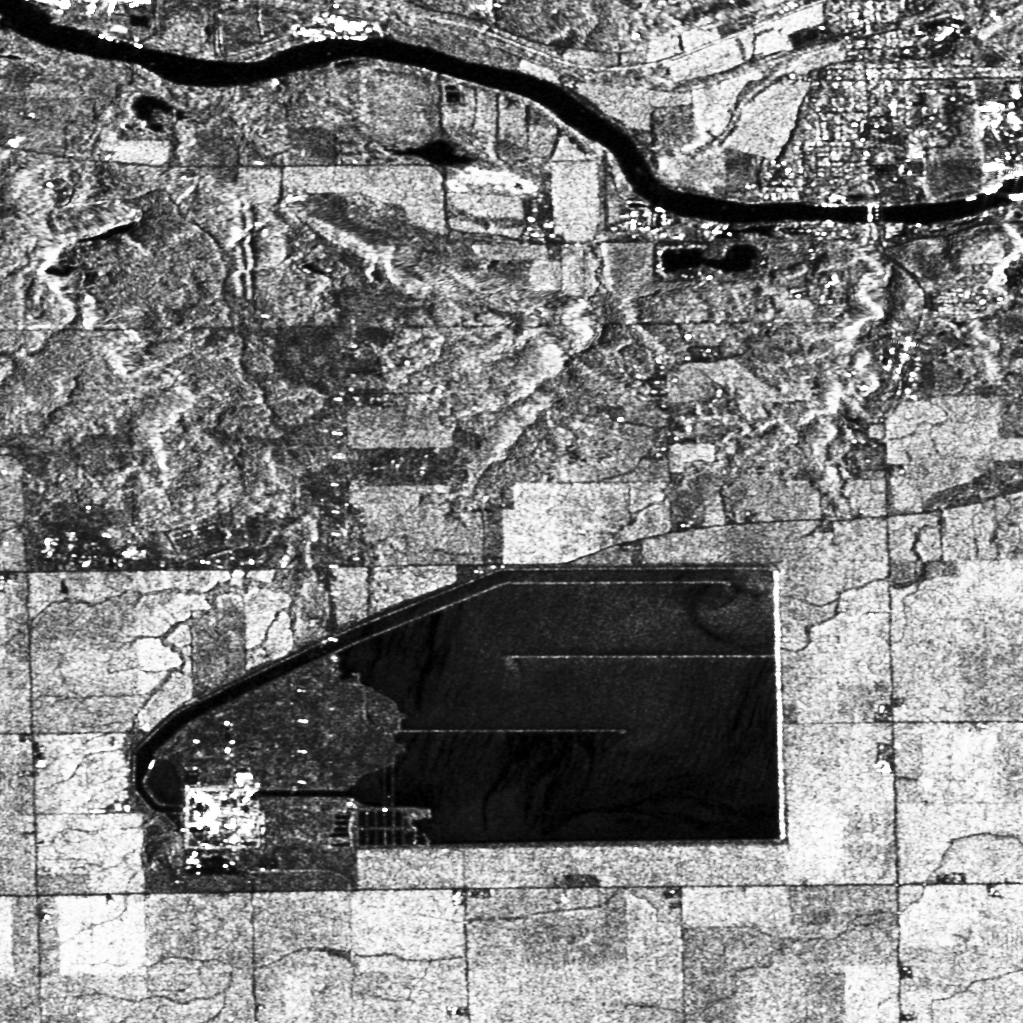
\includegraphics[width=\textwidth]{../../Figures/PNG/Illinois_1024_36L}
     \caption{Illinois-Region 2,  $L=36$}
    \label{fig:real_SAR_Images_coe-3}
  \end{subfigure}
  \caption{SAR images. }
  \label{fig:real_SAR_Images_coe}
\end{figure}



The three statistical tests are applied to the SAR images using
\(7\times 7\) local sliding windows, as illustrated in
Figures~\ref{fig:real_images_test_Mexico}, \ref{fig:test_lake}
and~\ref{fig:real_images_test_Illinois}.

The \(p\)-values obtained for each test are presented in
Figures~\ref{fig:Mexico_pvalue}, \ref{fig:lake_pvalue}
and~\ref{fig:Illinois_crops_pvalue}, respectively.

In Figures~\ref{fig:Mexico_crops_0.05}, \ref{fig:lake_0.05}
and~\ref{fig:Illinois_crops_0.05}, the maps of \(p\)-values composed of
a linear gradient of black and white colors, represent the decisions at
a \SI{5}{\percent} significance level.
Dark areas represent values below
\(0.05\), indicating evidence to reject the null hypothesis and
suggesting heterogeneity in these regions. 
In contrast, values above 0.05 are represented as white areas, indicating no evidence to reject
the fully-developed speckle hypothesis.
\begin{figure}[H]
  \centering
  \begin{subfigure}[b]{0.3\textwidth}
    \centering
    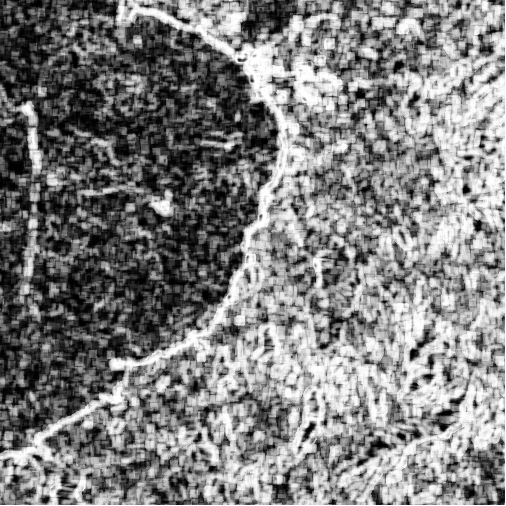
\includegraphics[width=\textwidth]{../../Figures/PNG/Entropy_Mexico_512_18L_AO_200b}
    \caption{$S_{\widetilde{H}_{\text{AO}}}(\bm{Z}; L)$}
    \label{fig:real_images_test_Mexico-1}
  \end{subfigure}
  \hfill
  \begin{subfigure}[b]{0.3\textwidth}
    \centering
    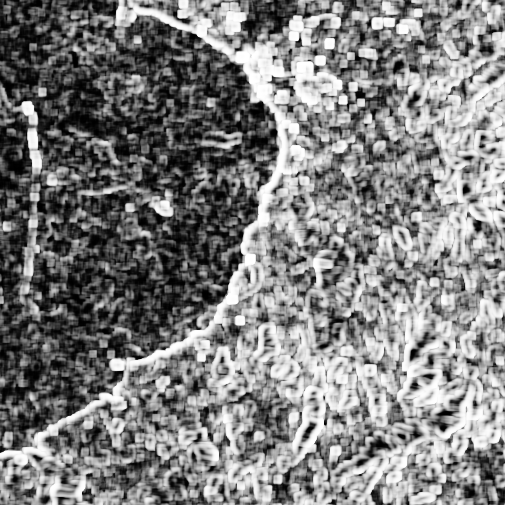
\includegraphics[width=\textwidth]{../../Figures/PNG/cv_mexico_512}
    \caption{$T_\text{CV}$}
    \label{fig:real_images_test_Mexico-2}
  \end{subfigure}
  \hfill
  \begin{subfigure}[b]{0.3\textwidth}
    \centering
    \includegraphics[width=\textwidth]{../../Figures/PNG/mnad_mexico_512}
    \caption{$T_{\text{CV}_{\text{MnAD}}}$}
    \label{fig:real_images_test_Mexico-3}
  \end{subfigure}
  \caption{Results of applying the test statistics to Coast of Jalisco image.}
  \label{fig:real_images_test_Mexico}
\end{figure}



\begin{figure}[H]
  \centering
  \begin{subfigure}[b]{0.3\textwidth}
    \centering
    \includegraphics[width=\textwidth]{../../Figures/PNG/H_pvalue_Mexico_512_18L_AO_200b}
    \caption{$S_{\widetilde{H}_{\text{AO}}}(\bm{Z}; L)$}
    \label{fig:Mexico_pvalue-1}
  \end{subfigure}
  \hfill
  \begin{subfigure}[b]{0.3\textwidth}
    \centering
    \includegraphics[width=\textwidth]{../../Figures/PNG/cv_pvalues_mexico_512}
    \caption{$T_\text{CV}$}
    \label{fig:Mexico_pvalue-2}
  \end{subfigure}
  \hfill
  \begin{subfigure}[b]{0.3\textwidth}
    \centering
    \includegraphics[width=\textwidth]{../../Figures/PNG/mnad_p_values_mexico_512}
     \caption{$T_{\text{CV}_{\text{MnAD}}}$}
    \label{fig:Mexico_pvalue-3}
  \end{subfigure}
  \caption{Map of $p$-values of Coast of Jalisco image for each test. }
  \label{fig:Mexico_pvalue}
\end{figure}



\begin{figure}[H]
  \centering
  \begin{subfigure}[b]{0.3\textwidth}
    \centering
    \includegraphics[width=\textwidth]{../../Figures/PNG/H_005__Mexico_512_18L_AO_200b}
    \caption{$S_{\widetilde{H}_{\text{AO}}}(\bm{Z}; L)$}
    \label{fig:Mexico_crops_0.05-1}
  \end{subfigure}
  \hfill
  \begin{subfigure}[b]{0.3\textwidth}
    \centering
    \includegraphics[width=\textwidth]{../../Figures/PNG/cv_005_pvalues_mexico_512}
    \caption{$T_\text{CV}$}
    \label{fig:Mexico_crops_0.05-2}
  \end{subfigure}
  \hfill
  \begin{subfigure}[b]{0.3\textwidth}
    \centering
    \includegraphics[width=\textwidth]{../../Figures/PNG/mnad_005_mexico_512}
     \caption{$T_{\text{CV}_{\text{MnAD}}}$}
    \label{fig:Mexico_crops_0.05-3}
  \end{subfigure}
  \caption{Results for a threshold of $0.05$ of the $p$-value of Coast of Jalisco for each test. }
  \label{fig:Mexico_crops_0.05}
\end{figure}



\begin{figure}[H]
  \centering
  \begin{subfigure}[b]{0.3\textwidth}
    \centering
    \includegraphics[width=\textwidth]{../../Figures/PNG/Entropy_lake_512_36L_AO_100b}
    \caption{$S_{\widetilde{H}_{\text{AO}}}(\bm{Z}; L)$}
    \label{fig:test_lake-1}
  \end{subfigure}
  \hfill
  \begin{subfigure}[b]{0.3\textwidth}
    \centering
    \includegraphics[width=\textwidth]{../../Figures/PNG/cv_lake_512}
    \caption{$T_\text{CV}$}
    \label{fig:test_lake-2}
  \end{subfigure}
  \hfill
  \begin{subfigure}[b]{0.3\textwidth}
    \centering
    \includegraphics[width=\textwidth]{../../Figures/PNG/mnad_lake_512}
    \caption{$T_{\text{CV}_{\text{MnAD}}}$}
    \label{fig:test_lake-3}
  \end{subfigure}
  \caption{Results of applying the test statistics, Illinois-Region 1.}
  \label{fig:test_lake}
\end{figure}



\begin{figure}[H]
  \centering
  \begin{subfigure}[b]{0.3\textwidth}
    \centering
    \includegraphics[width=\textwidth]{../../Figures/PNG/H_pvalue_lake_512_36L_AO_100b}
    \caption{$S_{\widetilde{H}_{\text{AO}}}(\bm{Z}; L)$}
    \label{fig:lake_pvalue-1}
  \end{subfigure}
  \hfill
  \begin{subfigure}[b]{0.3\textwidth}
    \centering
    \includegraphics[width=\textwidth]{../../Figures/PNG/cv_pvalues_lake_512}
    \caption{$T_\text{CV}$}
    \label{fig:lake_pvalue-2}
  \end{subfigure}
  \hfill
  \begin{subfigure}[b]{0.3\textwidth}
    \centering
    \includegraphics[width=\textwidth]{../../Figures/PNG/mnad_p_values_lake_512}
     \caption{$T_{\text{CV}_{\text{MnAD}}}$}
    \label{fig:lake_pvalue-3}
  \end{subfigure}
  \caption{Map of $p$-values, Illinois-Region 1. }
  \label{fig:lake_pvalue}
\end{figure}



\begin{figure}[H]
  \centering
  \begin{subfigure}[b]{0.3\textwidth}
    \centering
    \includegraphics[width=\textwidth]{../../Figures/PNG/H_005_lake_512_36L_AO_100b}
    \caption{$S_{\widetilde{H}_{\text{AO}}}(\bm{Z}; L)$}
    \label{fig:lake_0.05-1}
  \end{subfigure}
  \hfill
  \begin{subfigure}[b]{0.3\textwidth}
    \centering
    \includegraphics[width=\textwidth]{../../Figures/PNG/cv_005_pvalues_lake_512}
    \caption{$T_\text{CV}$}
    \label{fig:lake_0.05-2}
  \end{subfigure}
  \hfill
  \begin{subfigure}[b]{0.3\textwidth}
    \centering
    \includegraphics[width=\textwidth]{../../Figures/PNG/mnad_005_lake_512}
     \caption{$T_{\text{CV}_{\text{MnAD}}}$}
    \label{fig:lake_0.05-3}
  \end{subfigure}
  \caption{Results for a threshold of $0.05$ of the $p$-value, Illinois-Region 1. }
  \label{fig:lake_0.05}
\end{figure}




\begin{figure}[H]
  \centering
  \begin{subfigure}[b]{0.3\textwidth}
    \centering
    \includegraphics[width=\textwidth]{../../Figures/PNG/Entropy_Illinois_1024_36L_AO_200b}
    \caption{$S_{\widetilde{H}_{\text{AO}}}(\bm{Z}; L)$}
    \label{fig:real_images_test_Illinois-1}
  \end{subfigure}
  \hfill
  \begin{subfigure}[b]{0.3\textwidth}
    \centering
    \includegraphics[width=\textwidth]{../../Figures/PNG/cv_Illinois_crops_1024}
    \caption{$T_\text{CV}$}
    \label{fig:real_images_test_Illinois-2}
  \end{subfigure}
  \hfill
  \begin{subfigure}[b]{0.3\textwidth}
    \centering
    \includegraphics[width=\textwidth]{../../Figures/PNG/mnad_Illinois_crops_1024}
    \caption{$T_{\text{CV}_{\text{MnAD}}}$}
    \label{fig:real_images_test_Illinois-3}
  \end{subfigure}
  \caption{Results of applying the test statistics, Illinois-Region 2.}
  \label{fig:real_images_test_Illinois}
\end{figure}


\begin{figure}[H]
  \centering
  \begin{subfigure}[b]{0.3\textwidth}
    \centering
    \includegraphics[width=\textwidth]{../../Figures/PNG/H_pvalue_Illinois_1024_36L_AO_200b}
    \caption{$S_{\widetilde{H}_{\text{AO}}}(\bm{Z}; L)$}
    \label{fig:Illinois_crops_pvalue-1}
  \end{subfigure}
  \hfill
  \begin{subfigure}[b]{0.3\textwidth}
    \centering
    \includegraphics[width=\textwidth]{../../Figures/PNG/cv_pvalues_Illinois_crops_1024}
    \caption{$T_\text{CV}$}
    \label{fig:Illinois_crops_pvalue-2}
  \end{subfigure}
  \hfill
  \begin{subfigure}[b]{0.3\textwidth}
    \centering
    \includegraphics[width=\textwidth]{../../Figures/PNG/mnad_p_values_Illinois_crops_1024}
     \caption{$T_{\text{CV}_{\text{MnAD}}}$}
    \label{fig:Illinois_crops_pvalue-3}
  \end{subfigure}
  \caption{Map of $p$-values, Illinois-Region 2. }
  \label{fig:Illinois_crops_pvalue}
\end{figure}


\begin{figure}[H]
  \centering
  \begin{subfigure}[b]{0.3\textwidth}
    \centering
    \includegraphics[width=\textwidth]{../../Figures/PNG/H_005_pvalues_Illinois_1024_36L_AO_200b}
    \caption{$S_{\widetilde{H}_{\text{AO}}}(\bm{Z}; L)$}
    \label{fig:Illinois_crops_0.05-1}
  \end{subfigure}
  \hfill
  \begin{subfigure}[b]{0.3\textwidth}
    \centering
    \includegraphics[width=\textwidth]{../../Figures/PNG/cv_005_pvalues_Illinois_crops_1024}
    \caption{$T_\text{CV}$}
    \label{fig:Illinois_crops_0.05-2}
  \end{subfigure}
  \hfill
  \begin{subfigure}[b]{0.3\textwidth}
    \centering
    \includegraphics[width=\textwidth]{../../Figures/PNG/mnad_005_Illinois_crops_1024}
     \caption{$T_{\text{CV}_{\text{MnAD}}}$}
    \label{fig:Illinois_crops_0.05-3}
  \end{subfigure}
  \caption{Results for a threshold of $0.05$ of the $p$-value, Illinois-Region 2. }
  \label{fig:Illinois_crops_0.05}
\end{figure}



Using Shannon entropy is more meaningful than using the original and
robust CV to capture heterogeneity. It is justified that the dark areas
of the maps based on the \(T_\text{CV}\) and
\(T_{\text{CV}_{\text{MnAD}}}\) show coverage patterns similar to those
reported for the \(S_{\widetilde{H}_{\text{AO}}}(\bm{Z}; L)\) map. 
This suggests that although CV-based tests may produce slightly less
pronounced results than the entropy-based test, they still demonstrate a
comparable ability to detect heterogeneity within SAR images.

It is noticeable that the entropy and CV-based tools predicted
heterogeneity regions and boundaries where the statistical properties of
texture vary. The \(T_{\text{CV}_{\text{MnAD}}}\) test was shown to be
an effective edge detector. 
It emerges as a robust alternative to the classical CV test, making it less susceptible to the influence of
outliers and allowing it to produce more precise edges. 
Considering a
higher significance level may increase the sensitivity to edge detection
but also increase the risk of detecting false heterogeneous regions.

Additionally, assuming a \SI{5}{\percent} threshold for \(p\)-values, in
most cases, the heterogeneous regions detected by the
\(S_{\widetilde{H}{\text{AO}}}(\bm{Z}; L)\) test were more extensive
than those detected by the \(T_\text{CV}\) and
\(T_{\text{CV}_{\text{MnAD}}}\) tests. 
This was mainly observable in
Figures~\ref{fig:sim_SAR_Images_p05} \ref{fig:sim_SAR_Images_p05-1},
~\ref{fig:Mexico_crops_0.05} \ref{fig:Mexico_crops_0.05-1}, and~\ref{fig:lake_0.05} \ref{fig:lake_0.05-1}.
 
\chapter{Conclusions and future perspectives}\label{chp:conclusions}

This work provides a practical and theoretical answer to the
following physical question: How to detect heterogeneity in SAR images,
assuming that the SAR intensity follows the \(\Gamma_{\text{SAR}}\)
model. To this end, we proposed three novel hypothesis tests, one from
the Shannon entropy and two from the variation coefficient variants. The
performance of our proposals was evaluated using a Monte Carlo study.
The results showed that they were conservative in estimating the
probability of a type I error (false alarm rate) and the test power
(probability of detection), which increases with sample size. An
application to three recent SAR images was performed. The results showed
that the Shannon entropy-based test was more robust than the CV-based
tests. In addition, all tests could recognize images with different
textures and identify edges where the texture type changes.


\section*{Future perspectives}

For future research directions, there is a promising avenue in estimating the equivalent number of looks (ENL), a crucial parameter in the statistical modeling of multi-look synthetic aperture radar (SAR) imagery. This parameter serves as an indicator of heterogeneity and can significantly impact the accuracy of statistical analyses.

Additionally, we plan to explore the estimation of ENL in polarimetric SAR (PolSAR) data. This extension will involve:
\begin{itemize}
	\item Estimating the test on each of the three intensity channels of fully PolSAR data
	\item Analyzing the joint distribution
	\item Proposing techniques that generalize the test statistic  into the analysis of PolSAR data. 
		First, we can examine the entropy and CV of the distribution for the eigenvalues
		of the coherence matrix and then the Shannon entropy for the PolSAR matrix
			and trace-based versions for the CV of the PolSAR matrix.
\end{itemize}
%\include{todo}

%%
%% Parte pós-textual
%%
\backmatter

% Apêndices
% Comente se não houver apêndices
\newpage


%\appendix

%------------------------------------------------------------
%activar luego
    %\refstepcounter{chapter}
    %\chapter*{\appendixname\enskip\thechapter}
    %\addcontentsline{toc}{chapter}{\appendixname\enskip\thechapter}
    %
    %\section{Section in Appendix A}
	%
		
%
    \refstepcounter{chapter}
    %\chapter*{\appendixname\enskip\thechapter}
    %\addcontentsline{toc}{chapter}{\appendixname\enskip\thechapter}

    %\section{ Appendix A}
			%\chapter{Software and programs used in this thesis}  \label{appendix_software}
This PhD project required a vast amount of computing, preprocessing, analysis and plotting.
None of this would have been possible without the large number of different software packages used, all of which are free to use, and most of which are open source.
The following is a non-comprehensive list of the software used:
\begin{multicols}{2}
    \begin{description}
        \item[R] \citet{R}
        \item[CDO] \citet{CDO}
        \item[NCO] \citet{Zender2008}
        \item[Python] \citet{python}
        \item[netCDF] \citet{netcdf}
        \item[ScyPy] \citet{Jones2007}
        \item[GDAL] \citet{GDAL}
    \end{description}
\end{multicols}

Most of the data analysis and plotting was carried out using R. Several R packages were extremely useful and deserve a special mention:
\begin{multicols}{2}
    \begin{description}
 \item[ncdf4] \citet{ncdf4}
 \item[ggplot2] \citet{ggplot2}
 \item[patchwork] \citet{patchwork}
 \item[ggspatial] \citet{ggspatial}
% \item[ggalt] \citet{ggalt}
 \item[ggrepel] \citet{ggrepel}
 \item[RColorBrewer] \citet{RColorBrewer}
% \item[shinyjs] \citet{shinyjs}
% \item[shinydashboard] \citet{shinydashboard}
 \item[sf] \citet{sf}
 \item[stars] \citet{stars}
 \item[raster] \citet{raster}
 \item[rnaturalearth] \citet{rnaturalearth}
 \item[mapedit] \citet{mapedit}
 \item[leaflet] \citet{leaflet}
 \item[shiny] \citet{shiny}
 \item[dplyr] \citet{dplyr}
 \item[tidyr] \citet{tidyr}
 \item[glue] \citet{glue}
 \item[readr] \citet{readr}
 \item[profvis] \citet{profvis}
 \item[purrr] \citet{purrr}
 \item[furrr] \citet{furrr}
 \item[future] \citet{future}
 \item[futile.logger] \citet{futile.logger}
 \item[optparse] \citet{optparse}
 \item[lubridate] \citet{lubridate}
    \end{description}
\end{multicols}

This thesis was typeset in \LaTeX.

		%----------------------------------------
\cleardoublepage
%\newpage
% \phantomsection
%%------------------------------------
%%	ABBREVIATIONS
%%------------------------------------
%
%%\begin{abbreviations}{ll} % Include a list of abbreviations (a table of two columns)

\textbf{SAR} & Synthetic Aperture Radar\\
\textbf{UAVSAR} & Uninhabited Aerial Vehicle Synthetic Aperture Radar\\
\textbf{PDF} & Probability density function\\
\textbf{CDF} & Cumulative distribution function\\
\textbf{ASF} & Alaska Satellite Facility\\
\textbf{ESA} & Agencia Espacial Europea\\
\textbf{ASF} & Alaska Satellite Facility\\
\textbf{ENL} & Equivalent Number of Looks\\
\textbf{SNAP} & Sentinel Application Platform\\
\textbf{ROI} & Region of Interest\\ 
\textbf{ROC} & Receiver Operating Characteristic \\
\textbf{AUC} & Area Under the ROC Curve
\end{abbreviations}

%
%%------------------------------------
%{
  %\hypersetup{linkcolor=black}% para colocar color negro en la tabla de listas y figuras
  %
%
%\newpage
%\addcontentsline{toc}{chapter}{\listfigurename}
%\listoffigures
%\cleardoublepage
%\newpage
%\addcontentsline{toc}{chapter}{\listtablename}
%\listoftables
%
%}
% É aconselhável criar cada apêndice em um arquivo à parte, digamos
% "apendice1.tex", "apendice.tex", ... "apendiceM.tex" e depois
% incluí-los com:
% \include{apendice1}
% \include{apendice2}
% ...
% \include{apendiceM}
\newpage
\cleardoublepage
%------------------------------------
%	BIBLIOGRAPHY
%------------------------------------

%\bibliographystyle{IEEEtran}
%\bibliography{mendeley_v2}
%\nocite{*}
\printbibliography[heading=bibintoc]

%\setlength{\parskip}{3.0pt}
% Bibliografia
% É aconselhável utilizar o BibTeX a partir de um arquivo, digamos "biblio.bib".
% Para ajuda na criação do arquivo .bib e utilização do BibTeX, recorra ao
% BibTeXpress em www.cin.ufpe.br/~paguso/bibtexpress
%\nocite{*}
%\bibliographystyle{plain}
%\bibliography{biblio}

% Cólofon
% Descomente para incluir uma pequena nota com referência à UFPEThesis
%\colophon

%% Fim do documento
\end{document}
